\documentclass[12pt]{extarticle}
\usepackage[paperwidth=18in,paperheight=8.5in]{geometry}
\usepackage{amsmath}
\usepackage{hyperref}
\usepackage{multirow}
\usepackage{pdfpages}
\usepackage[utf8]{inputenc}
\title{Kaon mixing: chiral and continuum extrapolations}
\author{R Mukherjee}
\date{\today}
\begin{document}
\maketitle
\tableofcontents
\clearpage
\begin{figure}
\centering
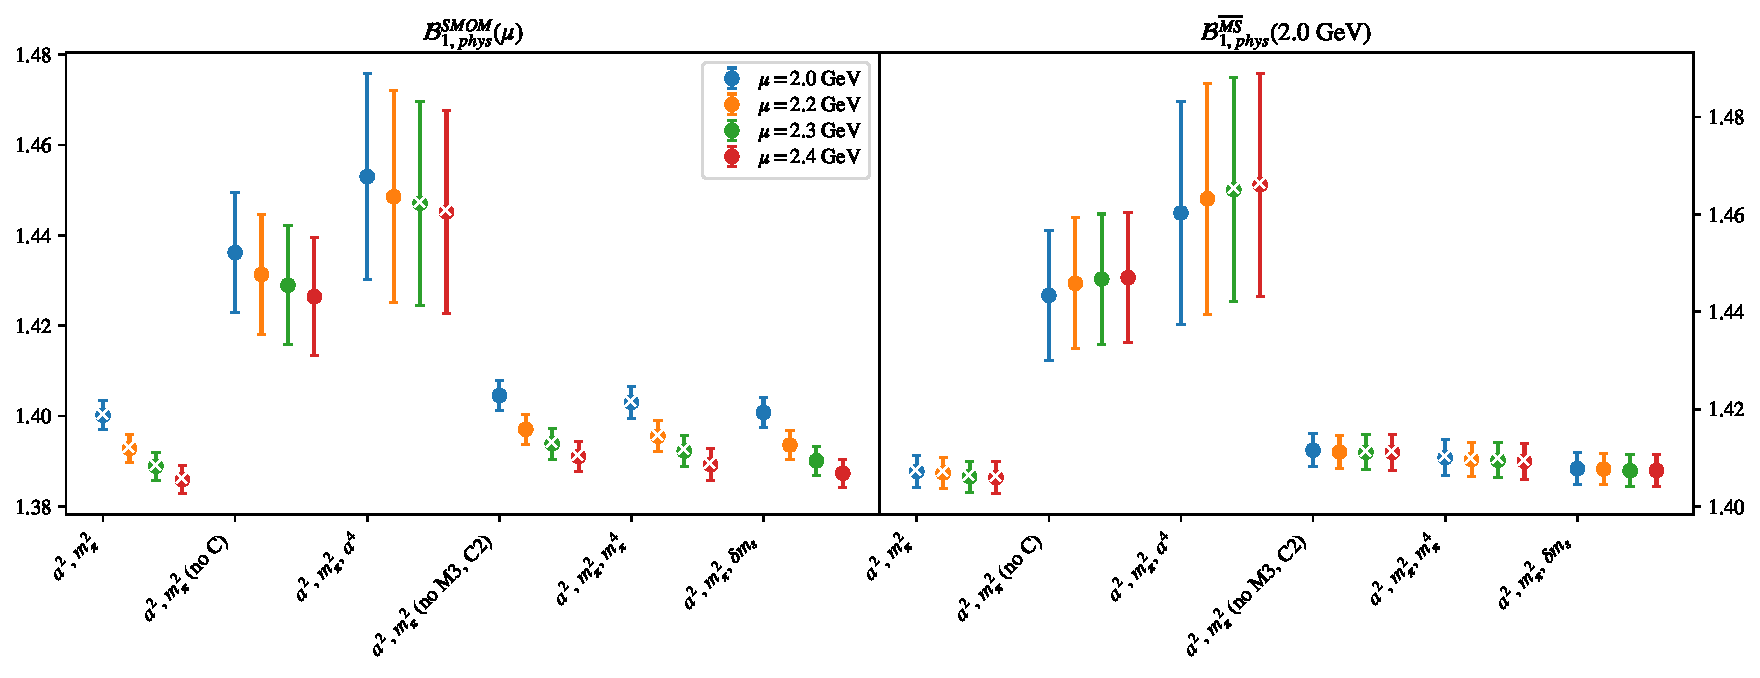
\includegraphics[page=1, width=1.1\textwidth]{VVpAA/NPR/fit_summary_bag.pdf}
\caption{$\mathcal{B}_{1}$\\(left) $\mathcal{B}_{phys}$ in RI/SMOM scheme from fit variations (fits with $p$-value $<0.05$ marked with ``$\times$"). \\(right) $\mathcal{B}_{phys}$ in $\overline{MS}$ computed using $\mathcal{B}^{\overline{MS}} = R^{\overline{MS}\leftarrow SMOM}(2.0)\sigma_{npt}(2.0,\mu) \mathcal{B}^{SMOM}(\mu)$.}
\end{figure}
\clearpage
\begin{figure}
\centering
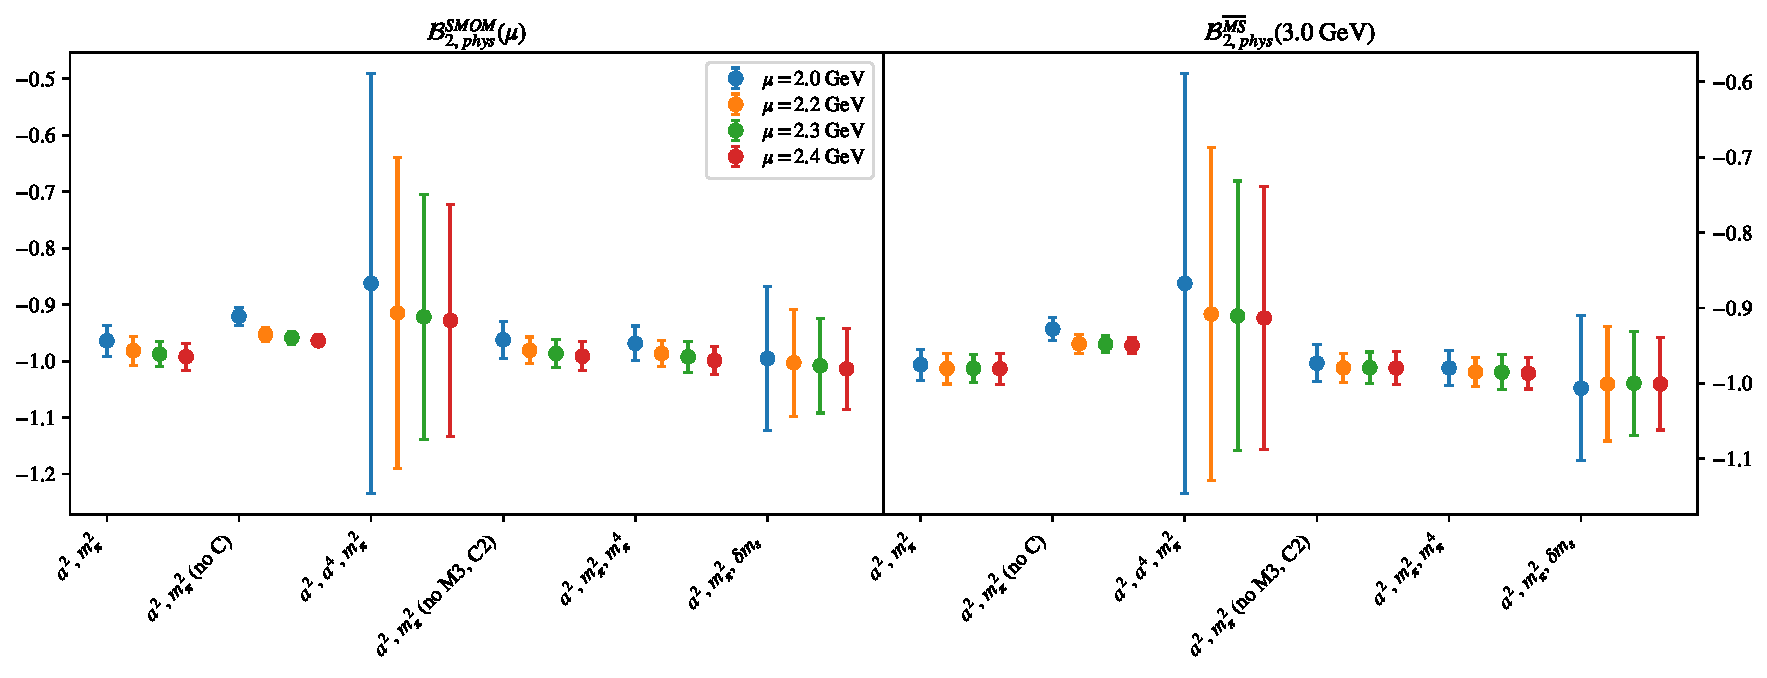
\includegraphics[page=1, width=1.1\textwidth]{VVmAA/NPR/fit_summary_bag.pdf}
\caption{$\mathcal{B}_{2}$\\(left) $\mathcal{B}_{phys}$ in RI/SMOM scheme from fit variations (fits with $p$-value $<0.05$ marked with ``$\times$"). \\(right) $\mathcal{B}_{phys}$ in $\overline{MS}$ computed using $\mathcal{B}^{\overline{MS}} = R^{\overline{MS}\leftarrow SMOM}(3.0)\sigma_{npt}(3.0,\mu) \mathcal{B}^{SMOM}(\mu)$.}
\end{figure}
\clearpage
\begin{figure}
\centering
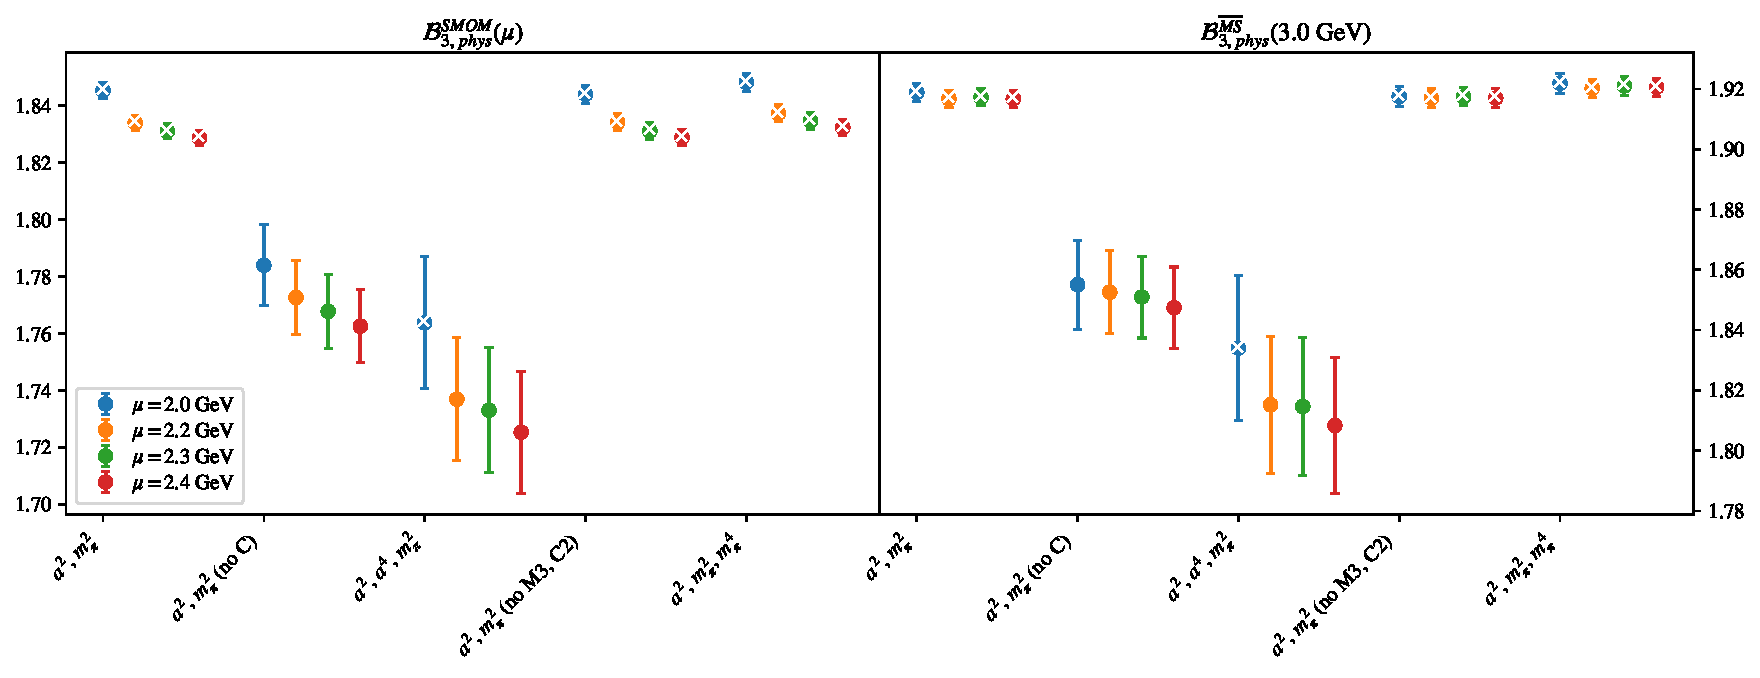
\includegraphics[page=1, width=1.1\textwidth]{SSmPP/NPR/fit_summary_bag.pdf}
\caption{$\mathcal{B}_{3}$\\(left) $\mathcal{B}_{phys}$ in RI/SMOM scheme from fit variations (fits with $p$-value $<0.05$ marked with ``$\times$"). \\(right) $\mathcal{B}_{phys}$ in $\overline{MS}$ computed using $\mathcal{B}^{\overline{MS}} = R^{\overline{MS}\leftarrow SMOM}(3.0)\sigma_{npt}(3.0,\mu) \mathcal{B}^{SMOM}(\mu)$.}
\end{figure}
\clearpage
\begin{figure}
\centering
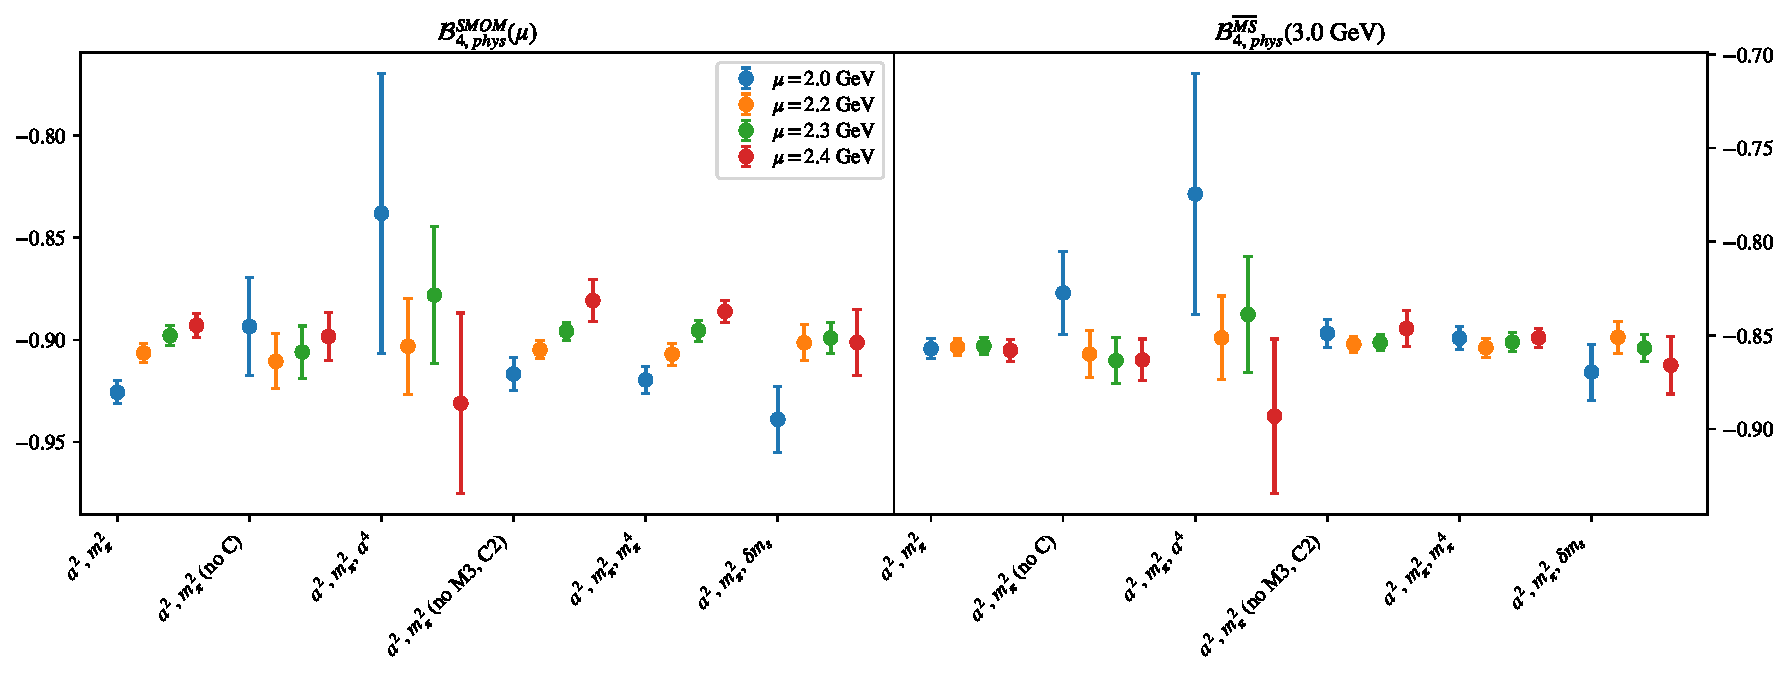
\includegraphics[page=1, width=1.1\textwidth]{SSpPP/NPR/fit_summary_bag.pdf}
\caption{$\mathcal{B}_{4}$\\(left) $\mathcal{B}_{phys}$ in RI/SMOM scheme from fit variations (fits with $p$-value $<0.05$ marked with ``$\times$"). \\(right) $\mathcal{B}_{phys}$ in $\overline{MS}$ computed using $\mathcal{B}^{\overline{MS}} = R^{\overline{MS}\leftarrow SMOM}(3.0)\sigma_{npt}(3.0,\mu) \mathcal{B}^{SMOM}(\mu)$.}
\end{figure}
\clearpage
\begin{figure}
\centering
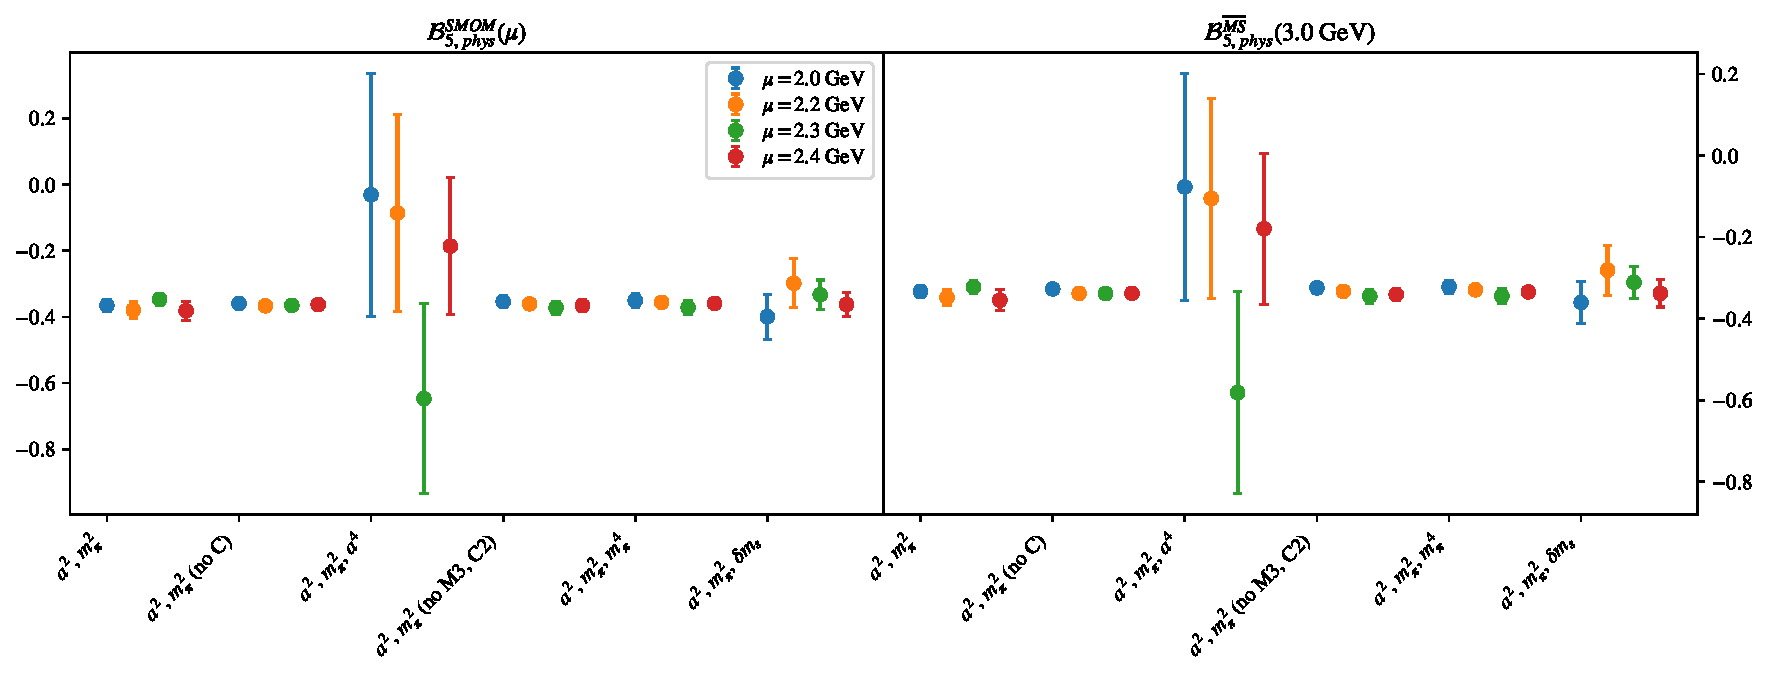
\includegraphics[page=1, width=1.1\textwidth]{TT/NPR/fit_summary_bag.pdf}
\caption{$\mathcal{B}_{5}$\\(left) $\mathcal{B}_{phys}$ in RI/SMOM scheme from fit variations (fits with $p$-value $<0.05$ marked with ``$\times$"). \\(right) $\mathcal{B}_{phys}$ in $\overline{MS}$ computed using $\mathcal{B}^{\overline{MS}} = R^{\overline{MS}\leftarrow SMOM}(3.0)\sigma_{npt}(3.0,\mu) \mathcal{B}^{SMOM}(\mu)$.}
\end{figure}
\clearpage
\section{$\mathcal{B}_1$}
\begin{table}[h!]
\begin{center}
\begin{tabular}{|c|c|c|c|c|c|c|}
\hline
$\mu$ (GeV) & $a^2$, $m_\pi^2$& $a^2$, $m_\pi^2$ (no C)& $a^2$, $m_\pi^2$, $a^4$& $a^2$, $m_\pi^2$ (no M3, C2)& $a^2$, $m_\pi^2$, $m_\pi^4$& $a^2$, $m_\pi^2$, $\delta m_s$\\
\hline
2.0& \hyperlink{VVpAA/NPR/a2m2_20.pdf.1}{\textbf{1.4032(28)}: 1.868 (0.096)} & \hyperlink{VVpAA/NPR/a2m2noC_20.pdf.1}{\textbf{1.414(13)}: 0.923 (0.397)} & \hyperlink{VVpAA/NPR/a2a4m2_20.pdf.1}{\textbf{1.421(21)}: 2.168 (0.07)} & \hyperlink{VVpAA/NPR/a2m2mcut_20.pdf.1}{\textbf{1.4070(37)}: 0.266 (0.85)} & \hyperlink{VVpAA/NPR/a2m2m4_20.pdf.1}{\textbf{1.4079(36)}: 0.699 (0.592)} & \hyperlink{VVpAA/NPR/a2m2delm_20.pdf.1}{\textbf{1.4013(32)}: 1.884 (0.11)}\\
2.2& \hyperlink{VVpAA/NPR/a2m2_22.pdf.1}{\textbf{1.3958(28)}: 2.201 (0.051)} & \hyperlink{VVpAA/NPR/a2m2noC_22.pdf.1}{\textbf{1.409(12)}: 1.165 (0.312)} & \hyperlink{VVpAA/NPR/a2a4m2_22.pdf.1}{\textbf{1.418(21)}: 2.512 (0.04)} & \hyperlink{VVpAA/NPR/a2m2mcut_22.pdf.1}{\textbf{1.3999(37)}: 0.363 (0.78)} & \hyperlink{VVpAA/NPR/a2m2m4_22.pdf.1}{\textbf{1.4007(36)}: 0.92 (0.451)} & \hyperlink{VVpAA/NPR/a2m2delm_22.pdf.1}{\textbf{1.3936(31)}: 2.14 (0.073)}\\
2.3& \hyperlink{VVpAA/NPR/a2m2_23.pdf.1}{\textbf{1.3925(28)}: 2.288 (0.043)} & \hyperlink{VVpAA/NPR/a2m2noC_23.pdf.1}{\textbf{1.407(12)}: 1.211 (0.298)} & \hyperlink{VVpAA/NPR/a2a4m2_23.pdf.1}{\textbf{1.416(21)}: 2.589 (0.035)} & \hyperlink{VVpAA/NPR/a2m2mcut_23.pdf.1}{\textbf{1.3967(37)}: 0.413 (0.743)} & \hyperlink{VVpAA/NPR/a2m2m4_23.pdf.1}{\textbf{1.3975(36)}: 0.988 (0.412)} & \hyperlink{VVpAA/NPR/a2m2delm_23.pdf.1}{\textbf{1.3901(31)}: 2.183 (0.068)}\\
2.4& \hyperlink{VVpAA/NPR/a2m2_24.pdf.1}{\textbf{1.3897(27)}: 2.337 (0.039)} & \hyperlink{VVpAA/NPR/a2m2noC_24.pdf.1}{\textbf{1.404(12)}: 1.236 (0.29)} & \hyperlink{VVpAA/NPR/a2a4m2_24.pdf.1}{\textbf{1.413(21)}: 2.65 (0.031)} & \hyperlink{VVpAA/NPR/a2m2mcut_24.pdf.1}{\textbf{1.3939(37)}: 0.415 (0.742)} & \hyperlink{VVpAA/NPR/a2m2m4_24.pdf.1}{\textbf{1.3947(36)}: 1.005 (0.404)} & \hyperlink{VVpAA/NPR/a2m2delm_24.pdf.1}{\textbf{1.3873(31)}: 2.232 (0.063)}\\
\hline
\end{tabular}
\caption{Physical point value from chiral and continuum extrapolation at renormalisation scale $\mu$. Entries are \textbf{value(error)}: $\chi^2/\text{DOF}$ ($p$-value).}
\end{center}
\end{table}
\begin{table}[h!]
\begin{center}
\begin{tabular}{|c c|c|c|c|c|c|c|}
\hline
$\mu$ (GeV) &  & $a^2$, $m_\pi^2$& $a^2$, $m_\pi^2$ (no C)& $a^2$, $m_\pi^2$, $a^4$& $a^2$, $m_\pi^2$ (no M3, C2)& $a^2$, $m_\pi^2$, $m_\pi^4$& $a^2$, $m_\pi^2$, $\delta m_s$\\
\hline
\multirow{3}{0.5in}{2.0} & $\alpha$ & 0.1001(98)& 0.056(54)& -0.02& 0.091(12)& 0.089(11)& 0.104(10)\\
 & $\beta$ & 0.00267(16)& 0.00244(32)& 0.00269(16)& 0.00209(35)& 0.00070(95)& 0.00276(17)\\
 & $\gamma$ &  &  & 0.24(28)&  & 0.000173(81)& -0.002(23)\\
\hline
\multirow{3}{0.5in}{2.2} & $\alpha$ & 0.1043(97)& 0.049(53)& -0.043& 0.094(12)& 0.092(11)& 0.109(10)\\
 & $\beta$ & 0.00266(15)& 0.00239(31)& 0.00268(15)& 0.00201(34)& 0.00057(95)& 0.00277(17)\\
 & $\gamma$ &  &  & 0.29(27)&  & 0.000182(81)& -0.003(23)\\
\hline
\multirow{3}{0.5in}{2.3} & $\alpha$ & 0.1058(97)& 0.046(53)& -0.051& 0.095(12)& 0.094(11)& 0.111(10)\\
 & $\beta$ & 0.00266(15)& 0.00239(31)& 0.00269(15)& 0.00201(34)& 0.00055(95)& 0.00278(17)\\
 & $\gamma$ &  &  & 0.31(27)&  & 0.000185(81)& -0.003(23)\\
\hline
\multirow{3}{0.5in}{2.4} & $\alpha$ & 0.1064(97)& 0.047(53)& -0.049& 0.096(12)& 0.094(11)& 0.112(10)\\
 & $\beta$ & 0.00268(15)& 0.00239(31)& 0.00270(15)& 0.00202(34)& 0.00055(95)& 0.00279(17)\\
 & $\gamma$ &  &  & 0.31(27)&  & 0.000186(81)& -0.003(23)\\
\hline
\end{tabular}
\caption{Fit values of coefficients in $Q = Q_{phys} + \mathbf{\alpha} a^2 + \mathbf{\beta}\left(\frac{m_\pi^2}{f_\pi^2}-\frac{m_{\pi,PDG}^2}{f_\pi^2}\right) + \gamma(\ldots)$}
\end{center}
\end{table}
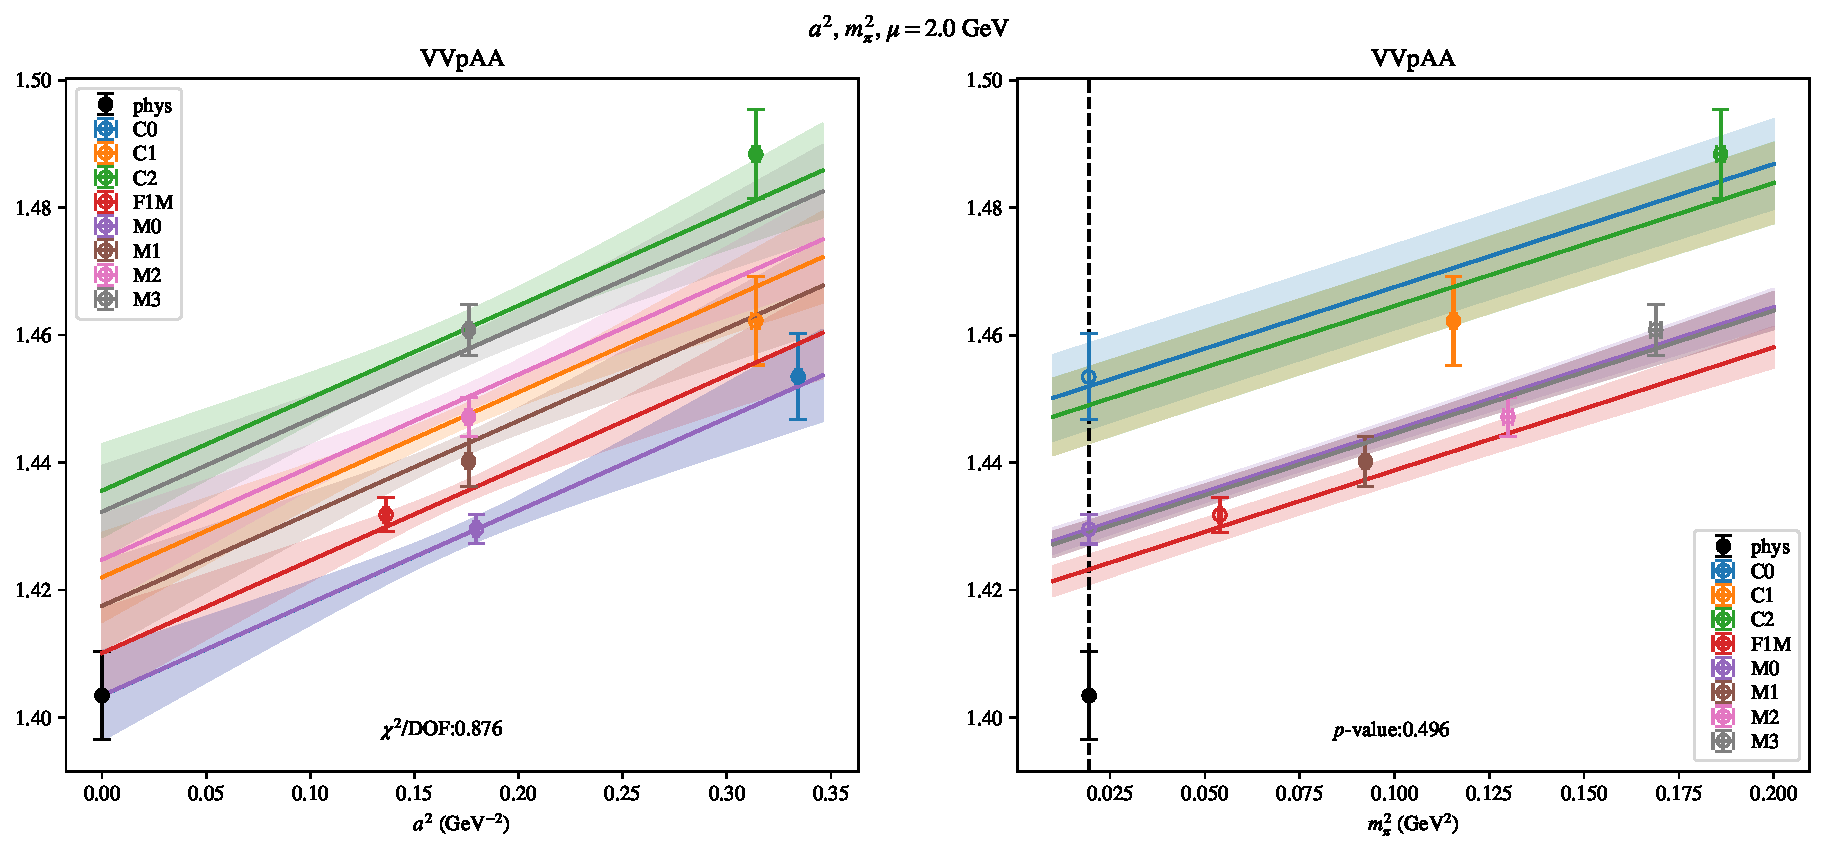
\includepdf[link, pages=-]{VVpAA/NPR/a2m2_20.pdf}
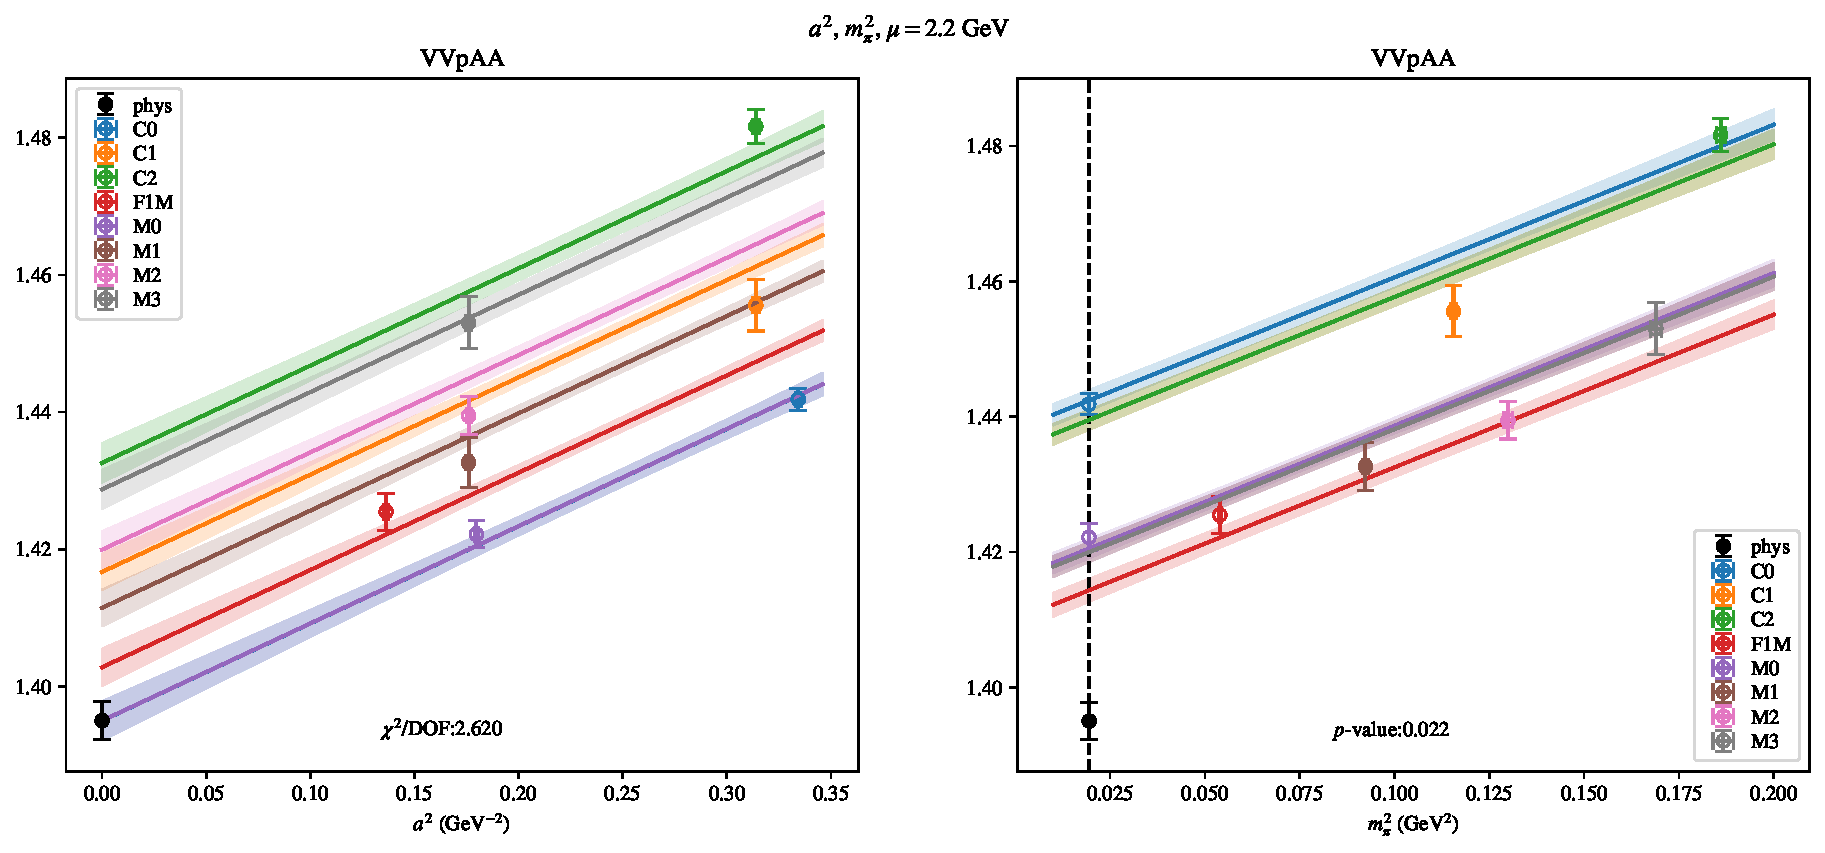
\includepdf[link, pages=-]{VVpAA/NPR/a2m2_22.pdf}
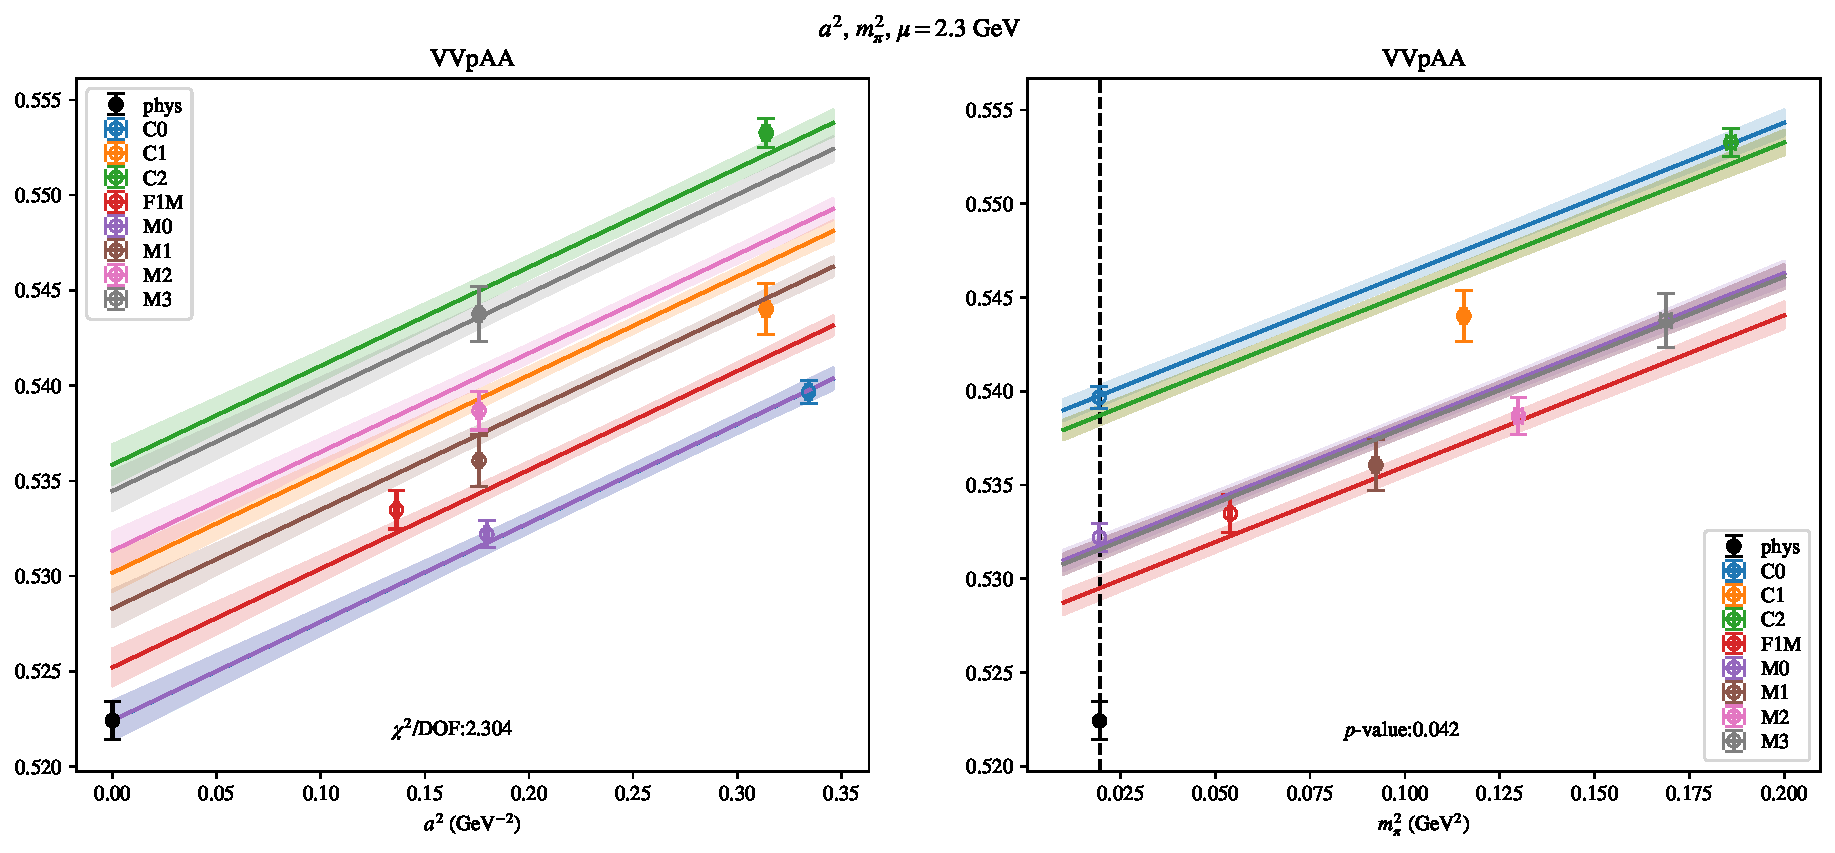
\includepdf[link, pages=-]{VVpAA/NPR/a2m2_23.pdf}
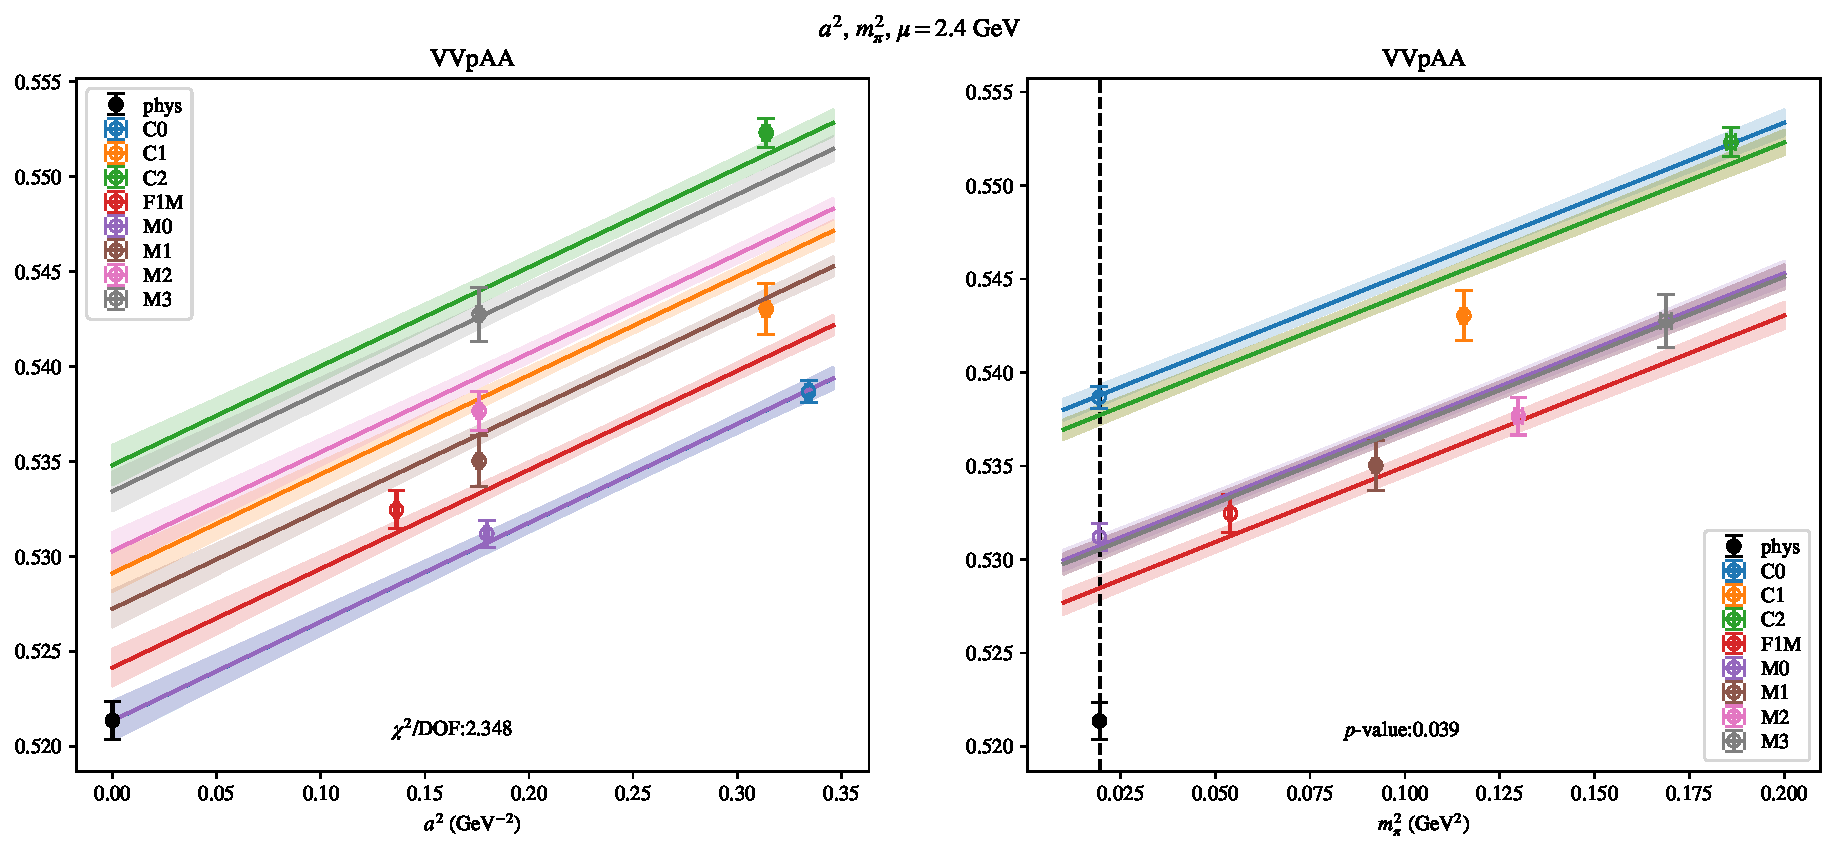
\includepdf[link, pages=-]{VVpAA/NPR/a2m2_24.pdf}
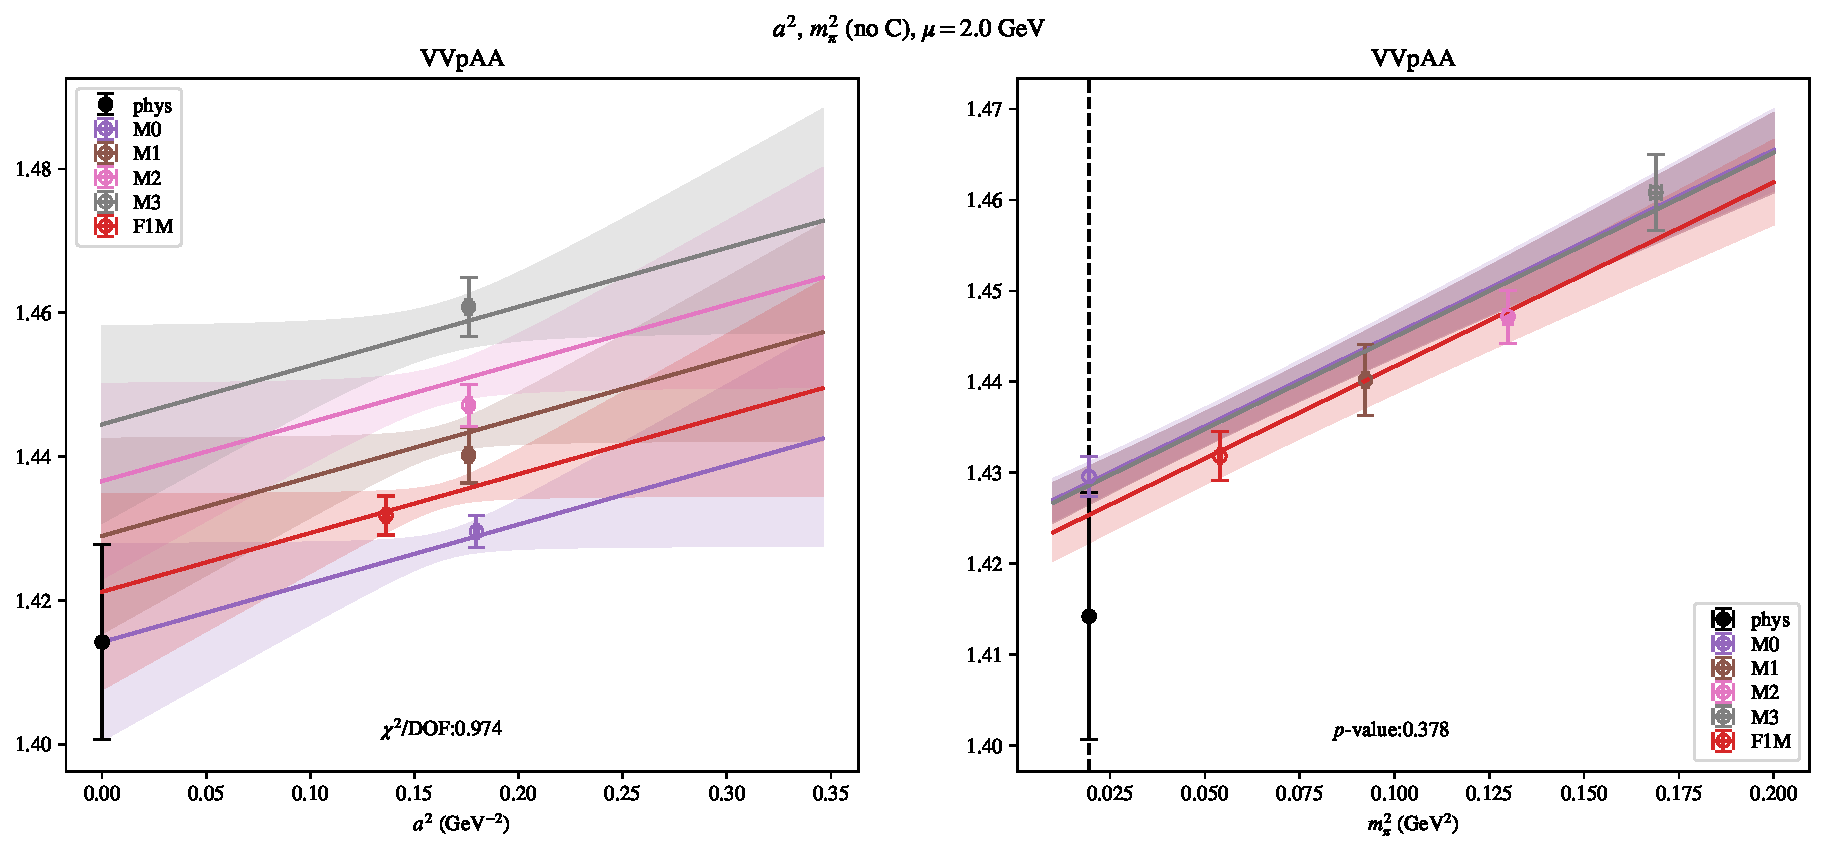
\includepdf[link, pages=-]{VVpAA/NPR/a2m2noC_20.pdf}
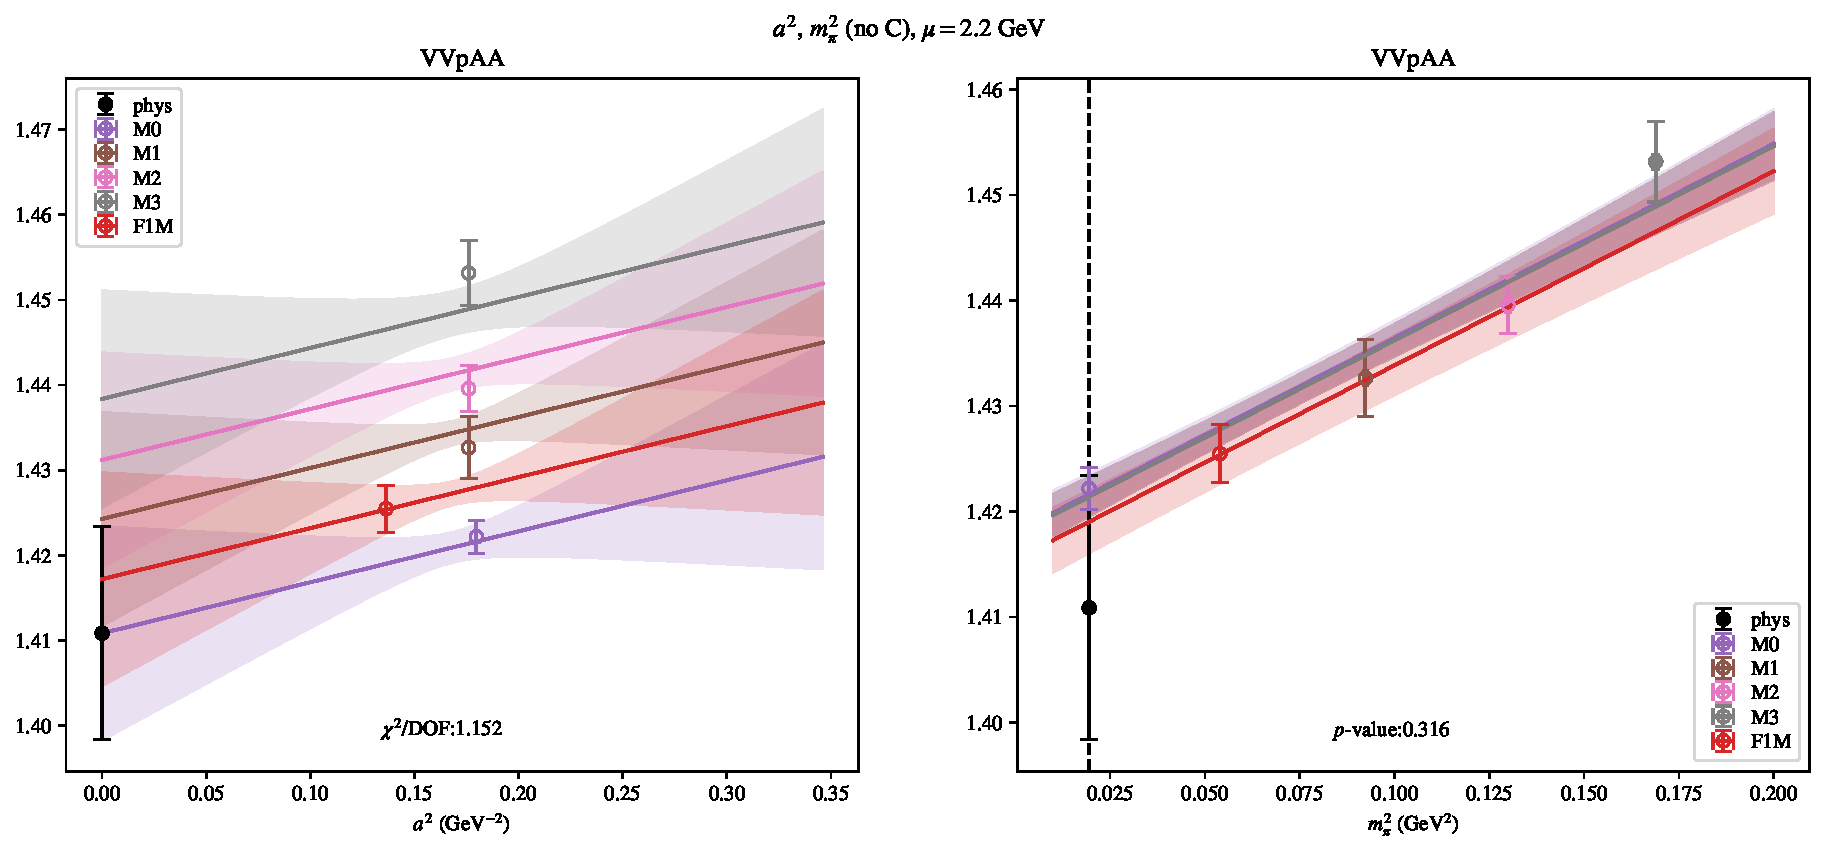
\includepdf[link, pages=-]{VVpAA/NPR/a2m2noC_22.pdf}
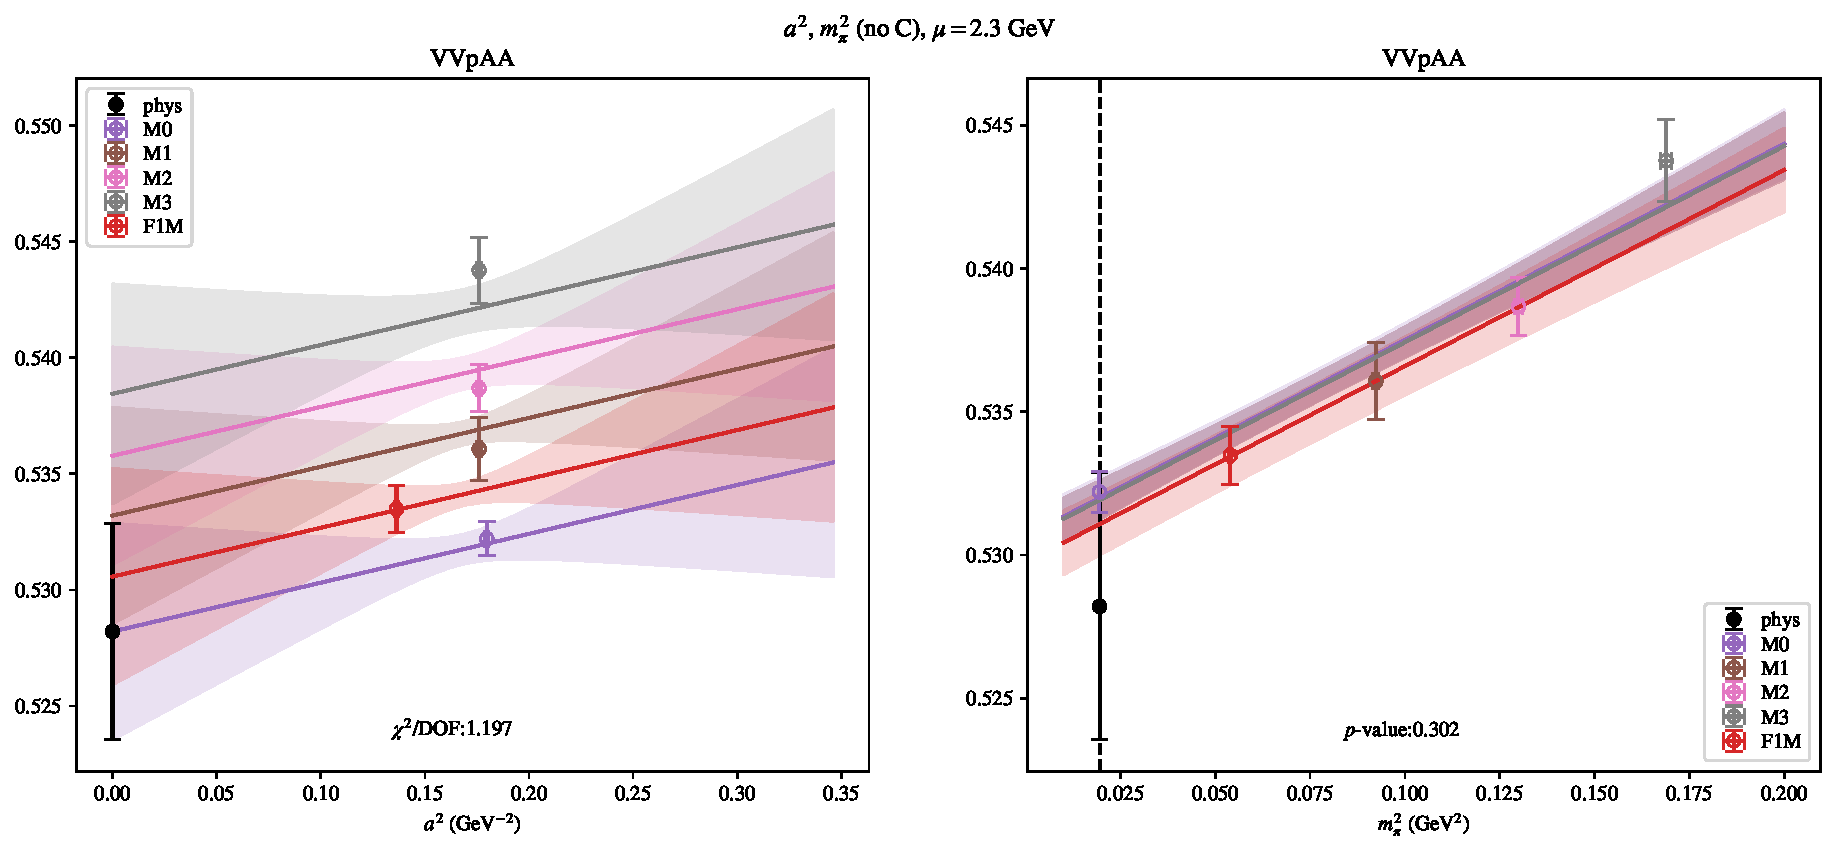
\includepdf[link, pages=-]{VVpAA/NPR/a2m2noC_23.pdf}
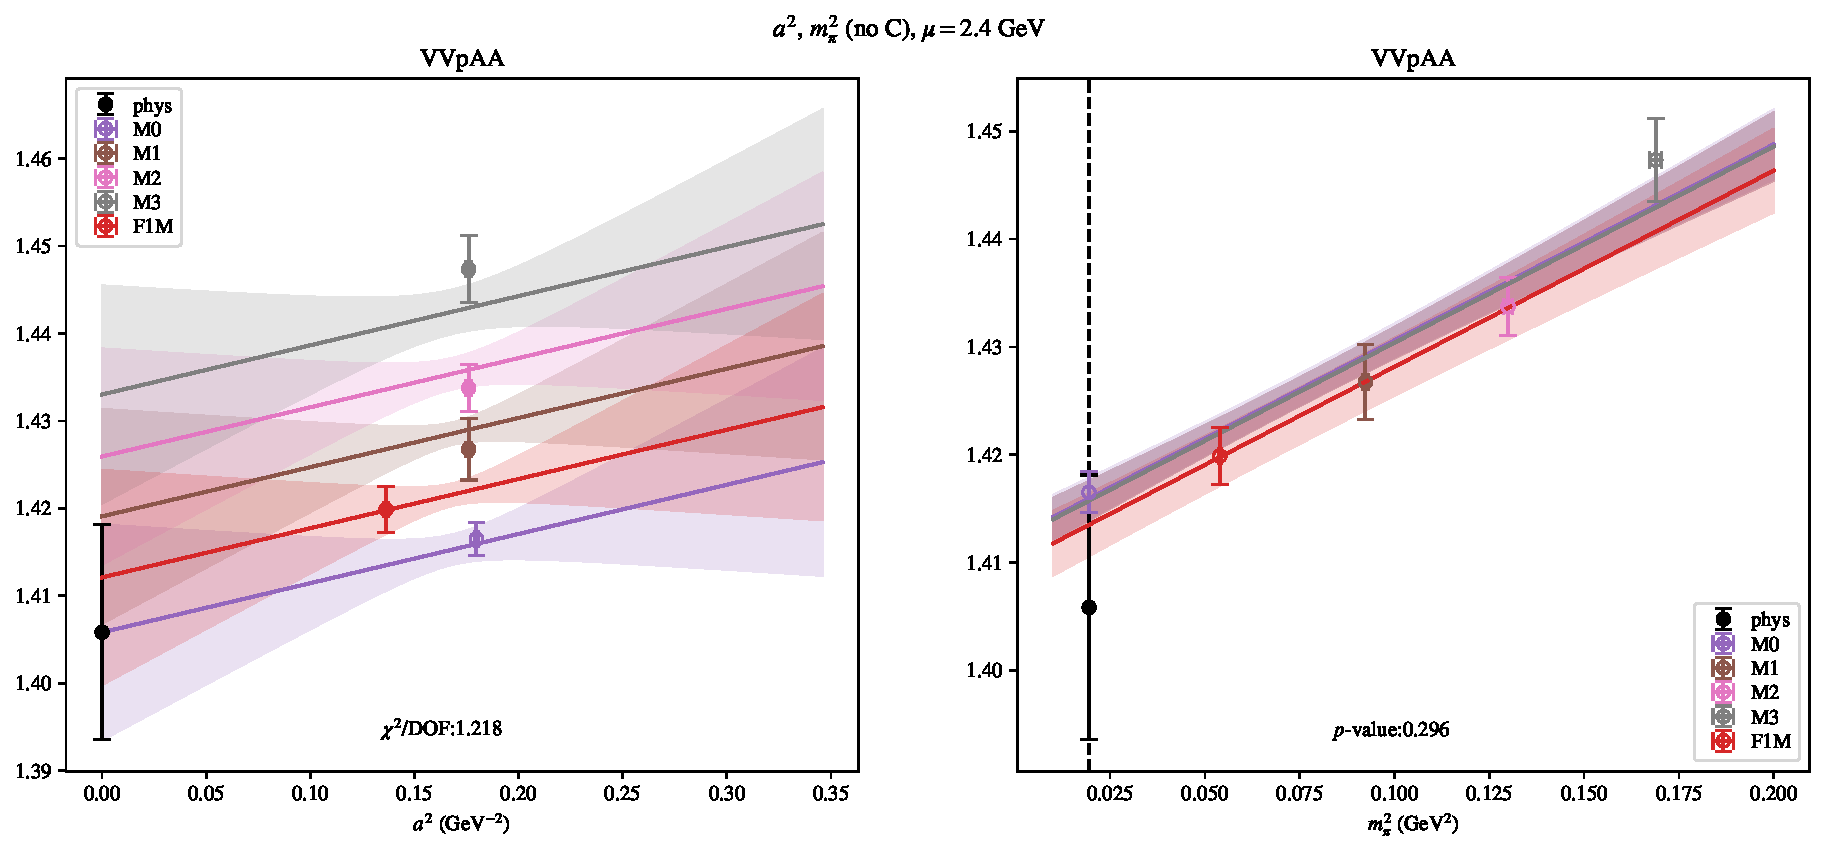
\includepdf[link, pages=-]{VVpAA/NPR/a2m2noC_24.pdf}
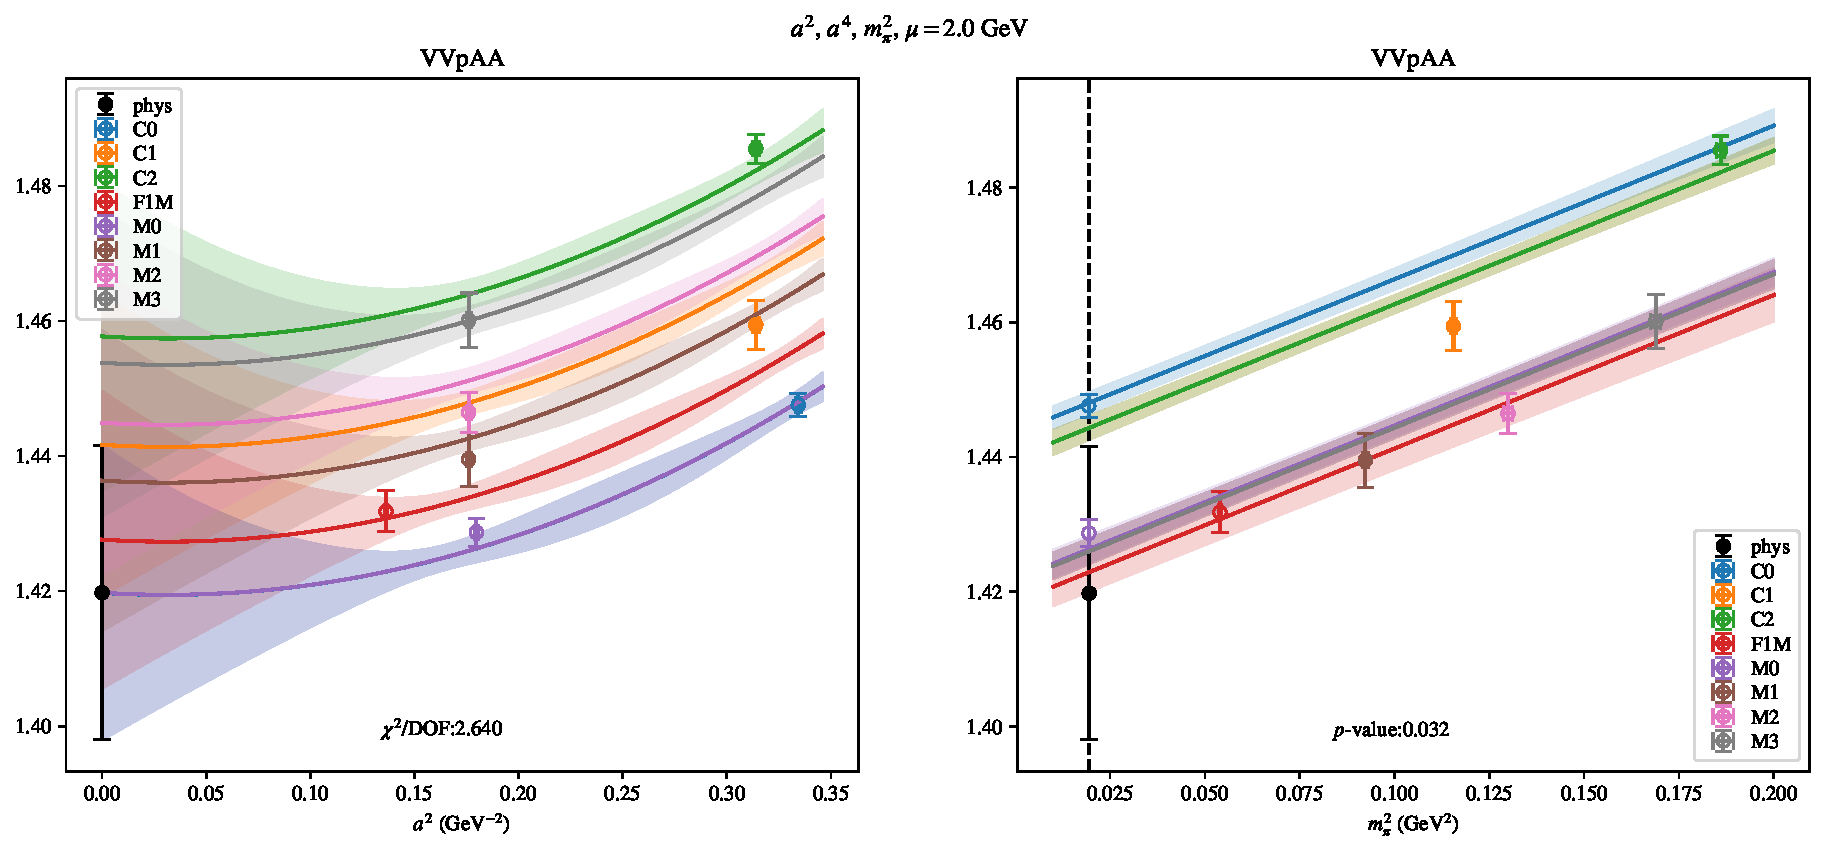
\includepdf[link, pages=-]{VVpAA/NPR/a2a4m2_20.pdf}
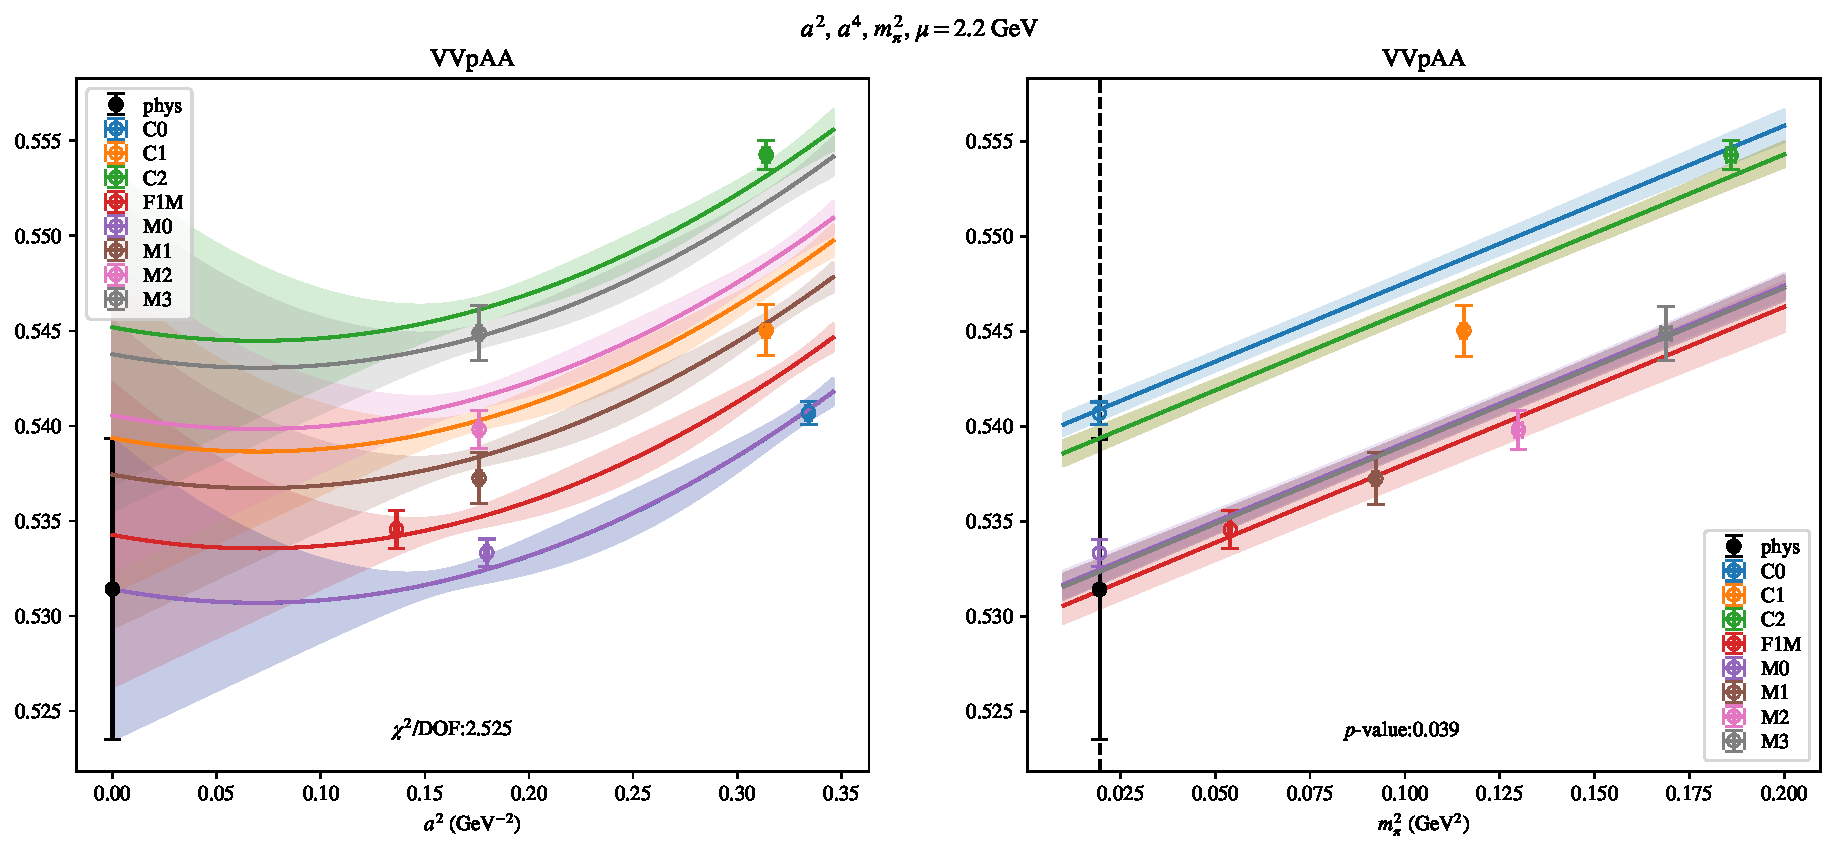
\includepdf[link, pages=-]{VVpAA/NPR/a2a4m2_22.pdf}
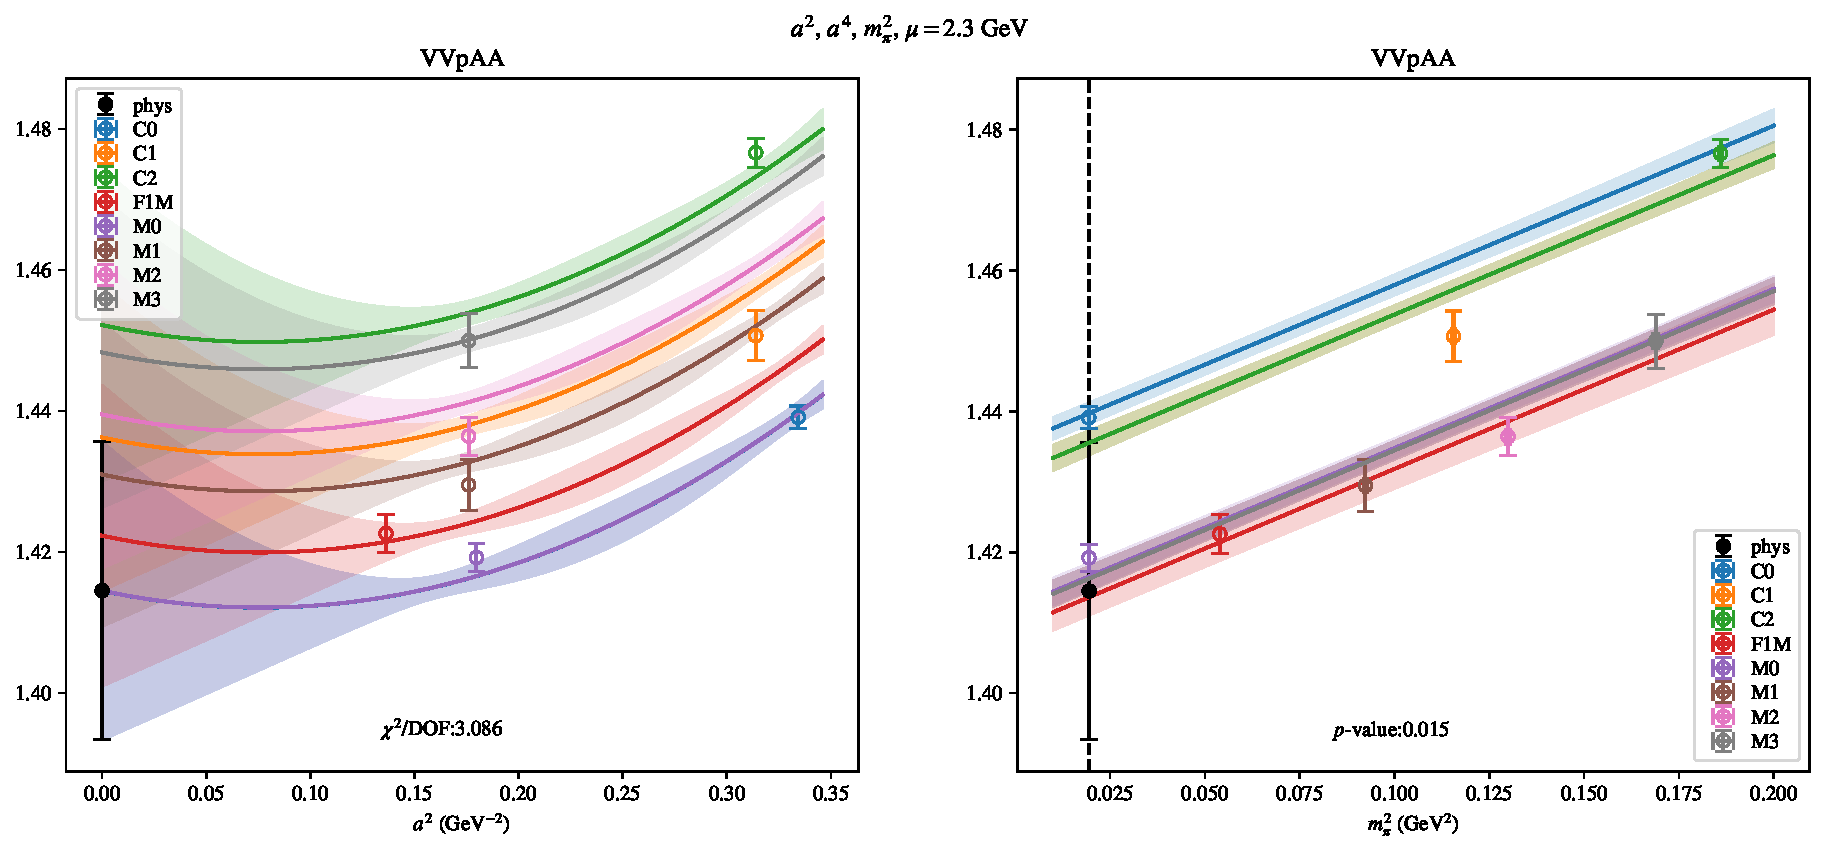
\includepdf[link, pages=-]{VVpAA/NPR/a2a4m2_23.pdf}
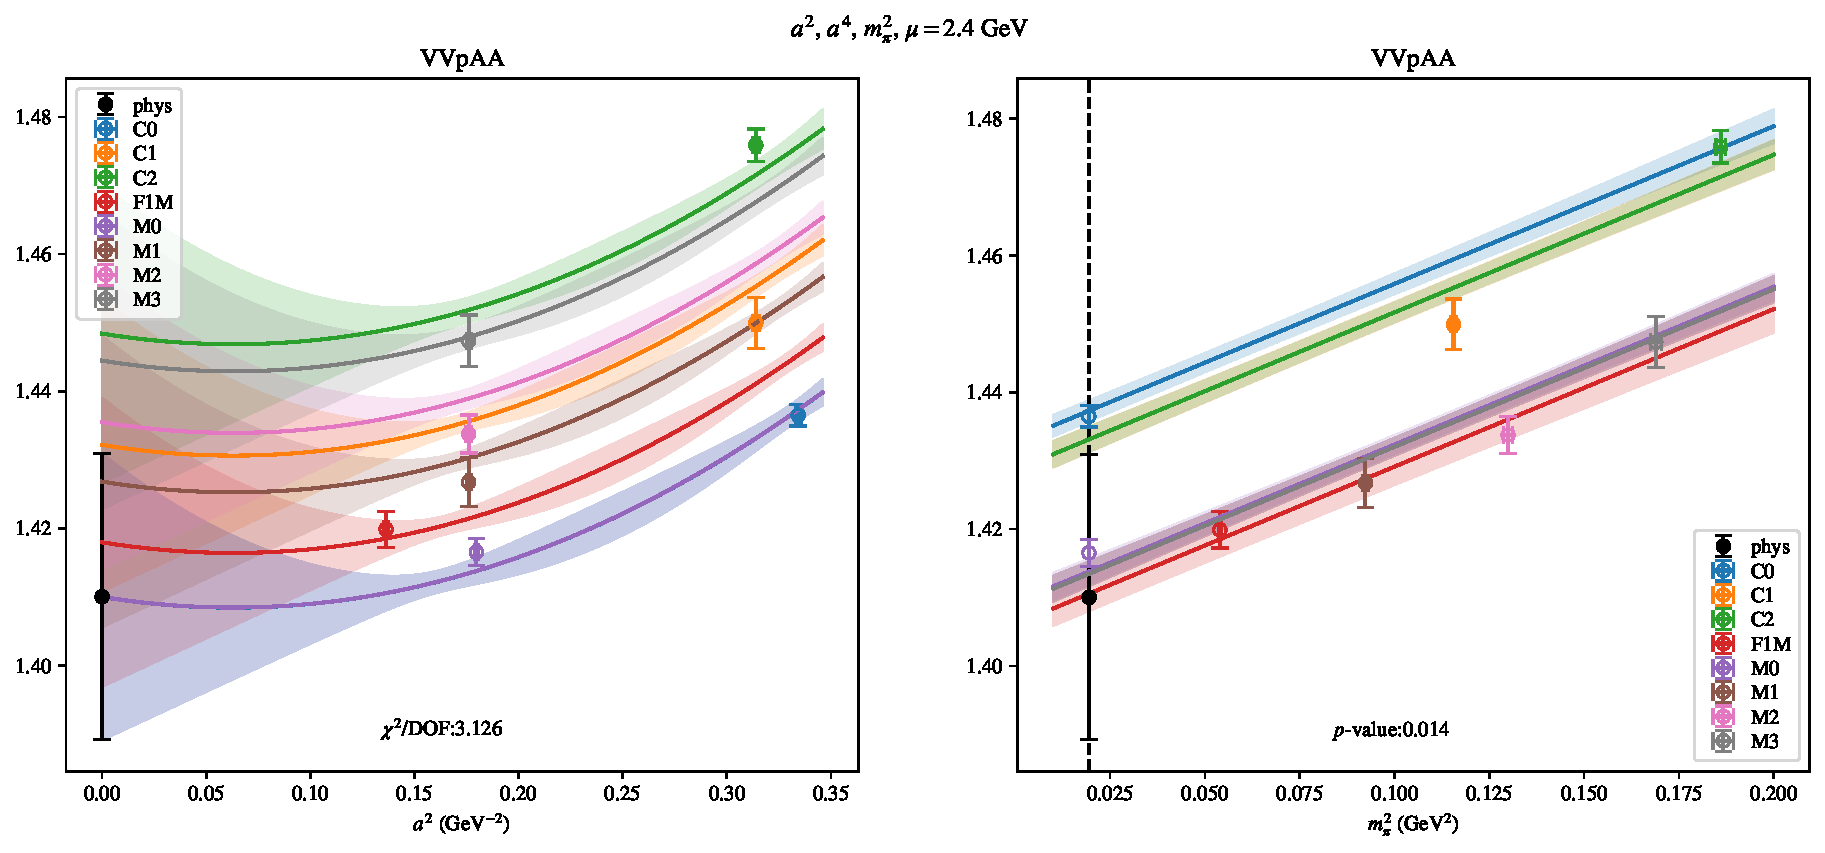
\includepdf[link, pages=-]{VVpAA/NPR/a2a4m2_24.pdf}
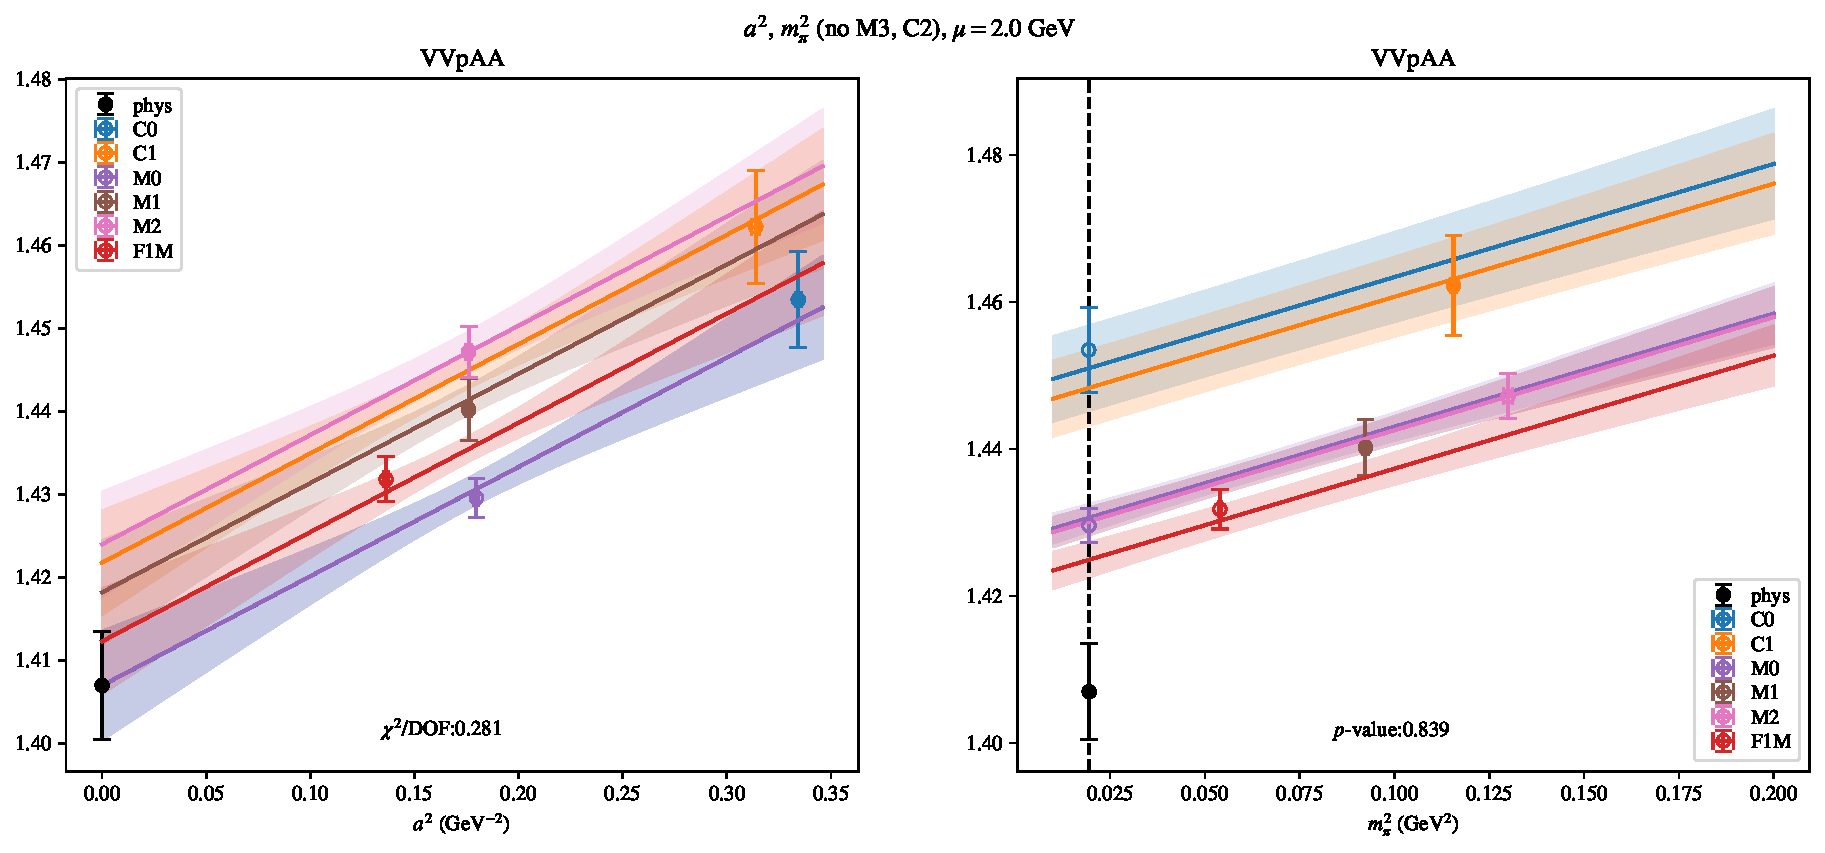
\includepdf[link, pages=-]{VVpAA/NPR/a2m2mcut_20.pdf}
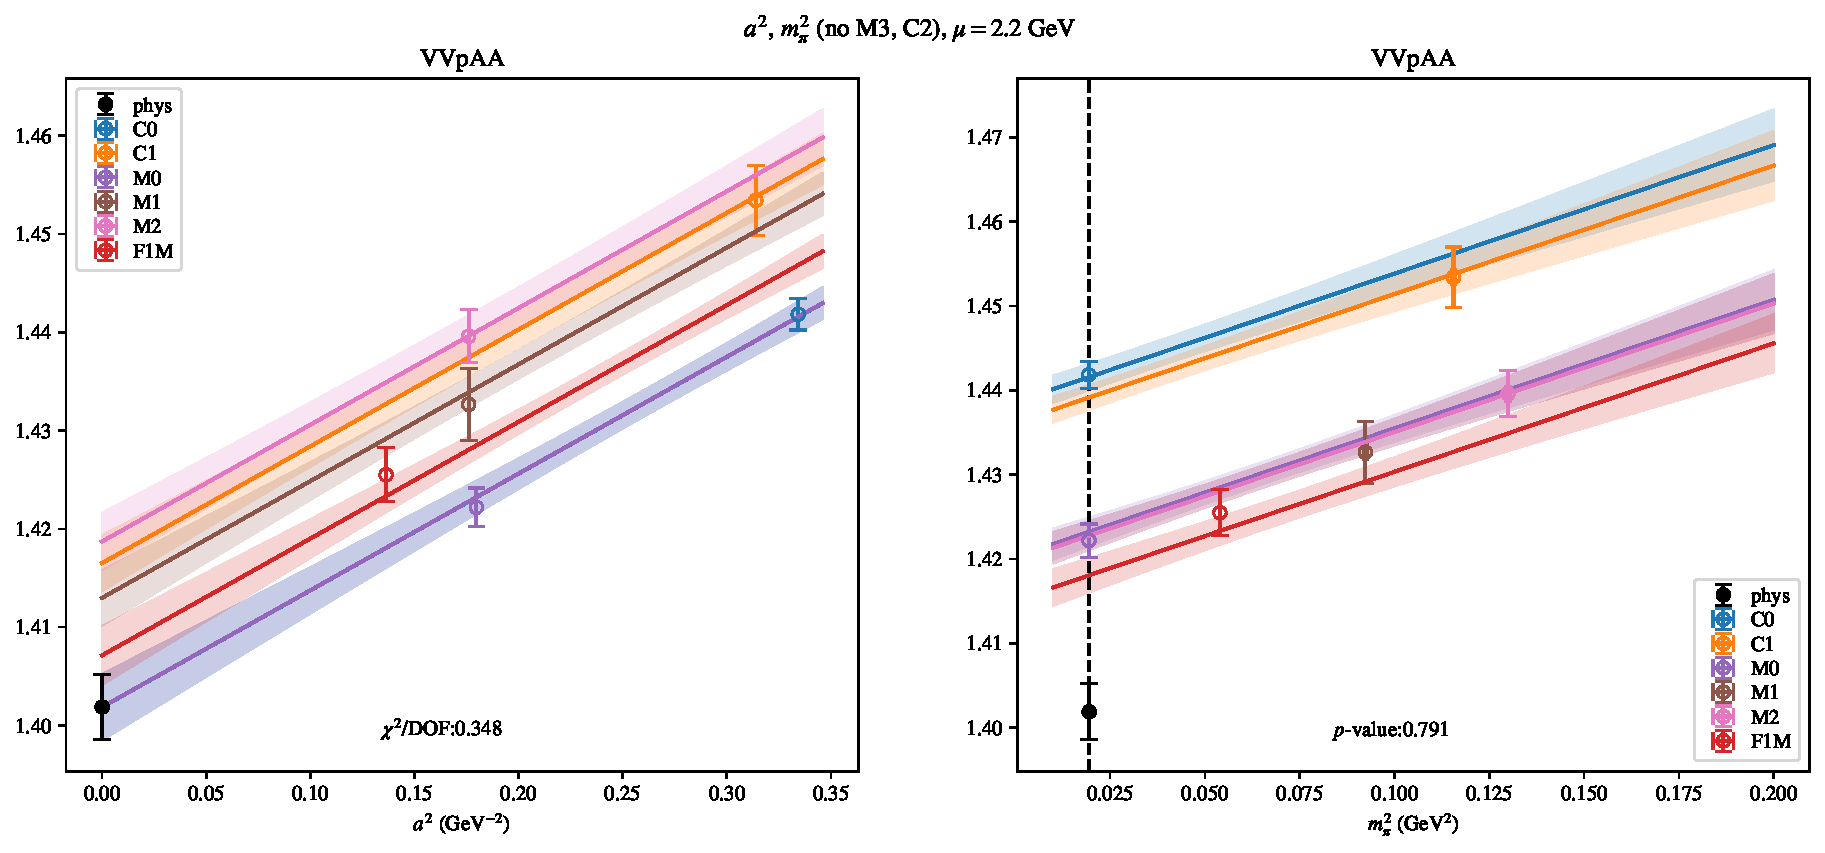
\includepdf[link, pages=-]{VVpAA/NPR/a2m2mcut_22.pdf}
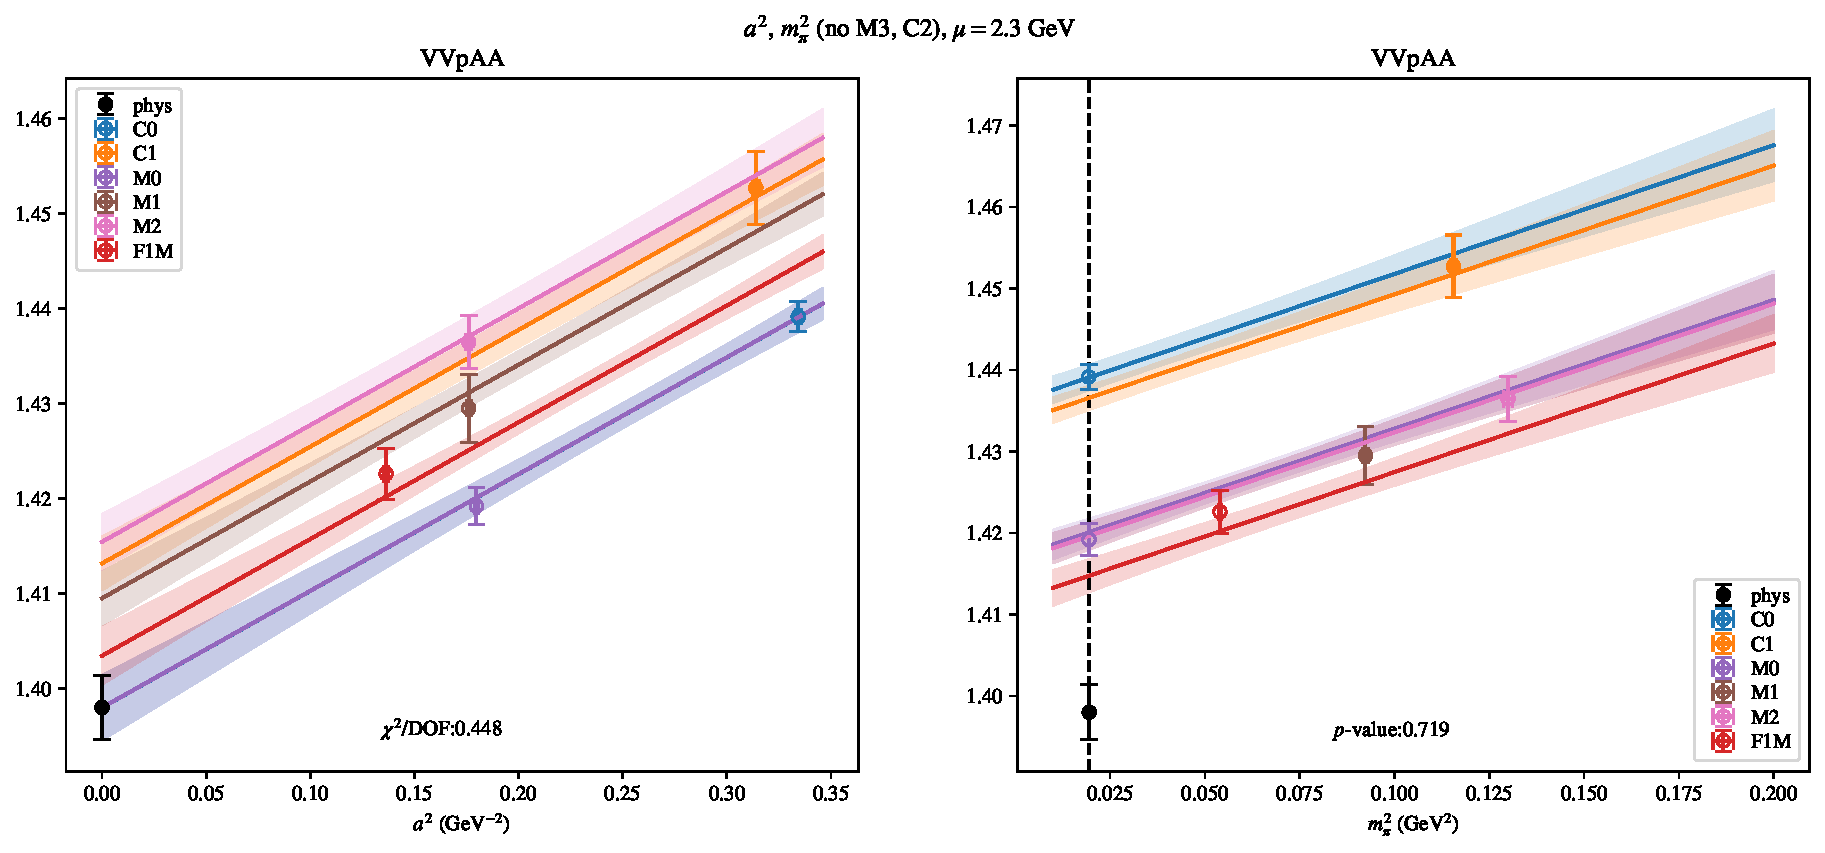
\includepdf[link, pages=-]{VVpAA/NPR/a2m2mcut_23.pdf}
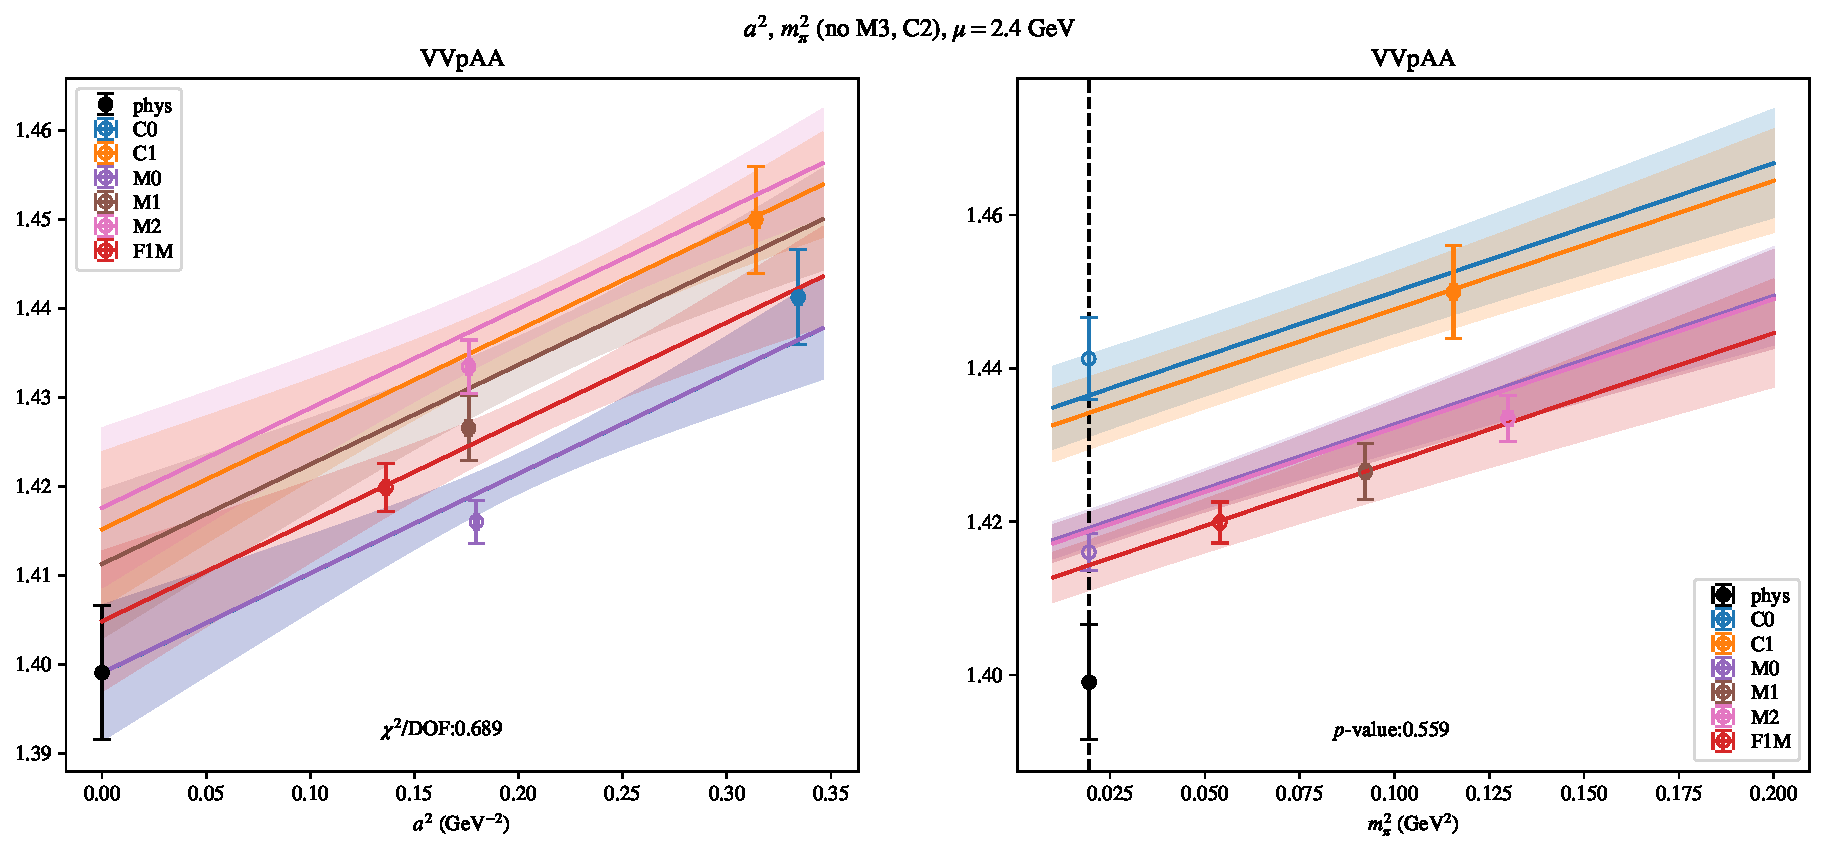
\includepdf[link, pages=-]{VVpAA/NPR/a2m2mcut_24.pdf}
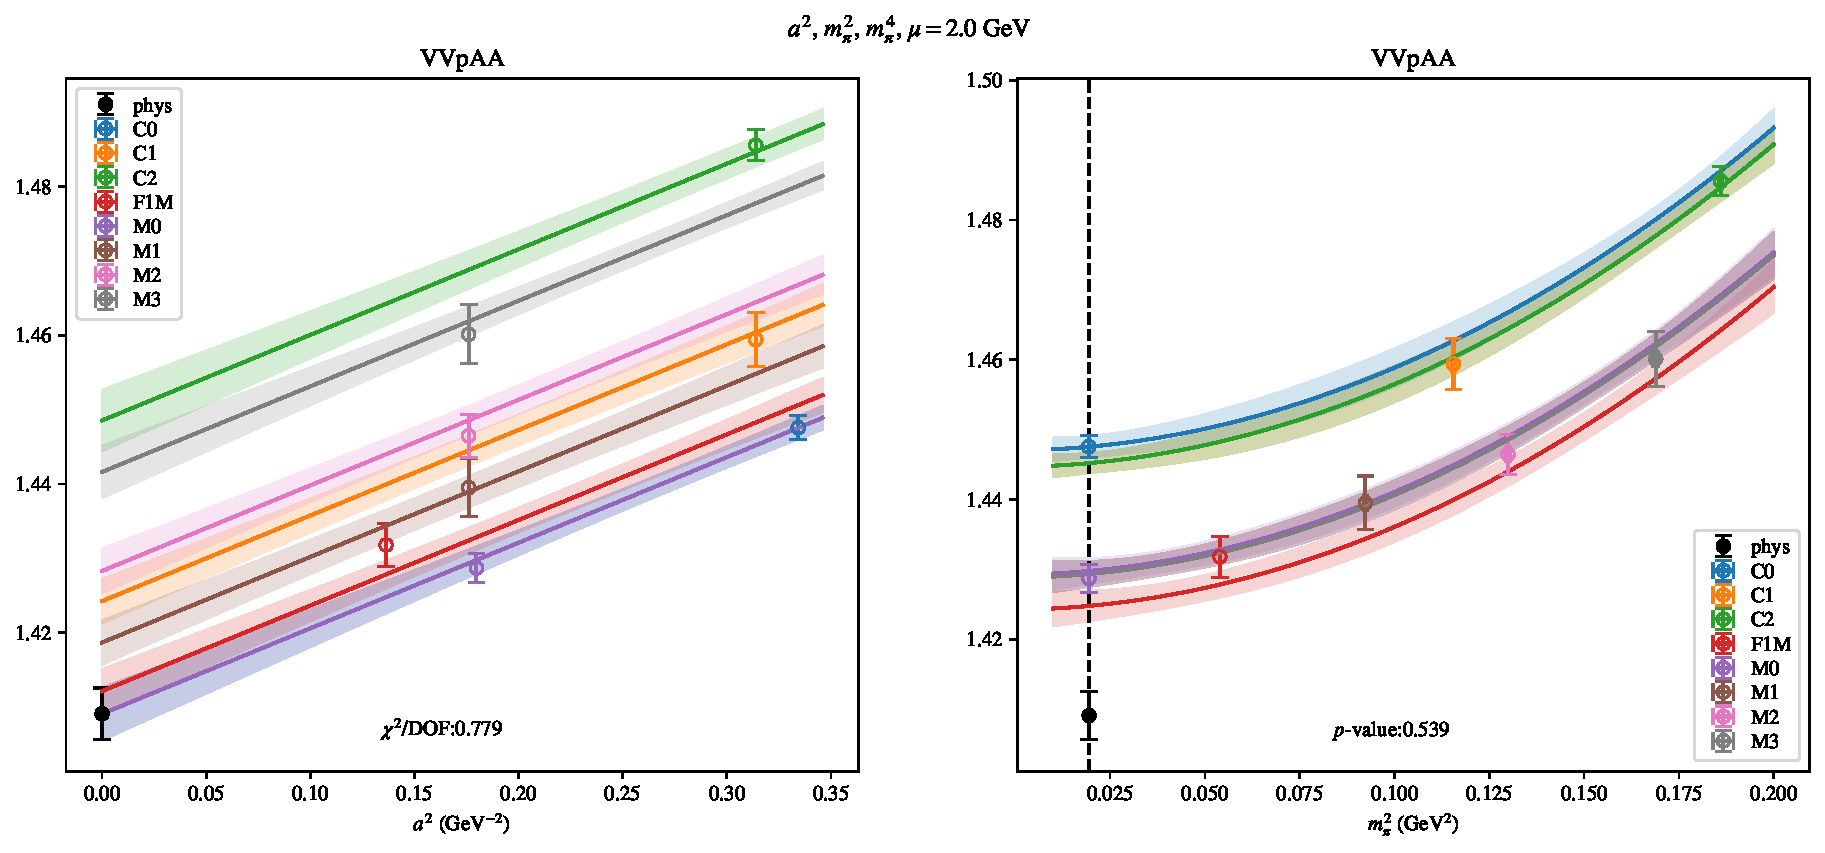
\includepdf[link, pages=-]{VVpAA/NPR/a2m2m4_20.pdf}
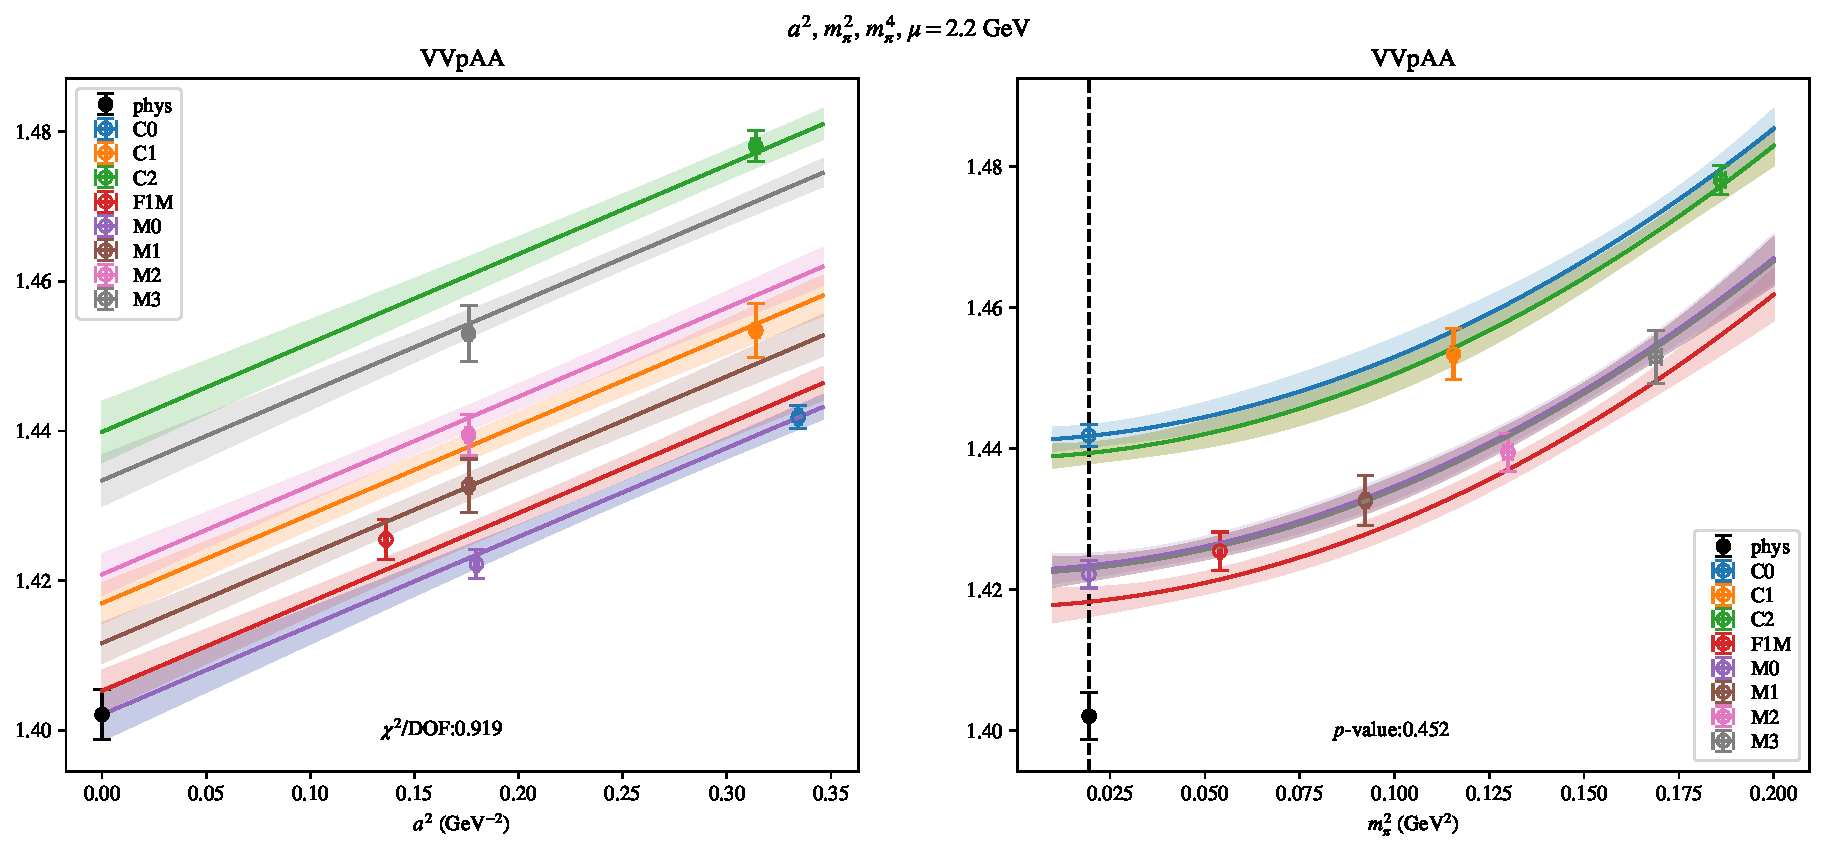
\includepdf[link, pages=-]{VVpAA/NPR/a2m2m4_22.pdf}
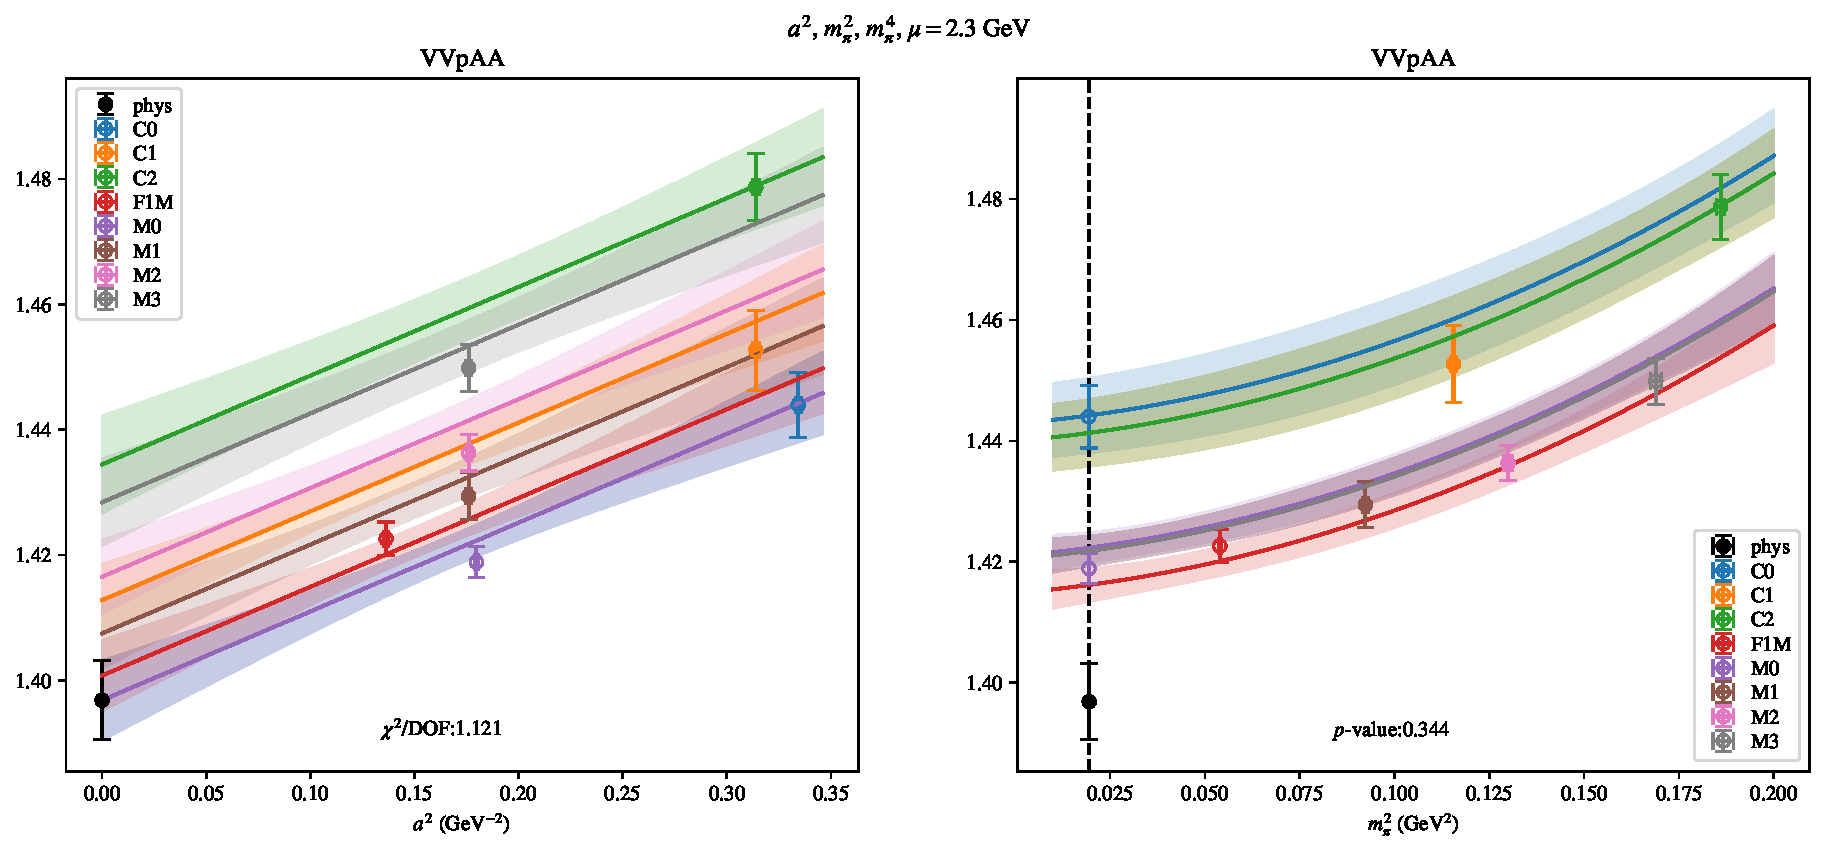
\includepdf[link, pages=-]{VVpAA/NPR/a2m2m4_23.pdf}
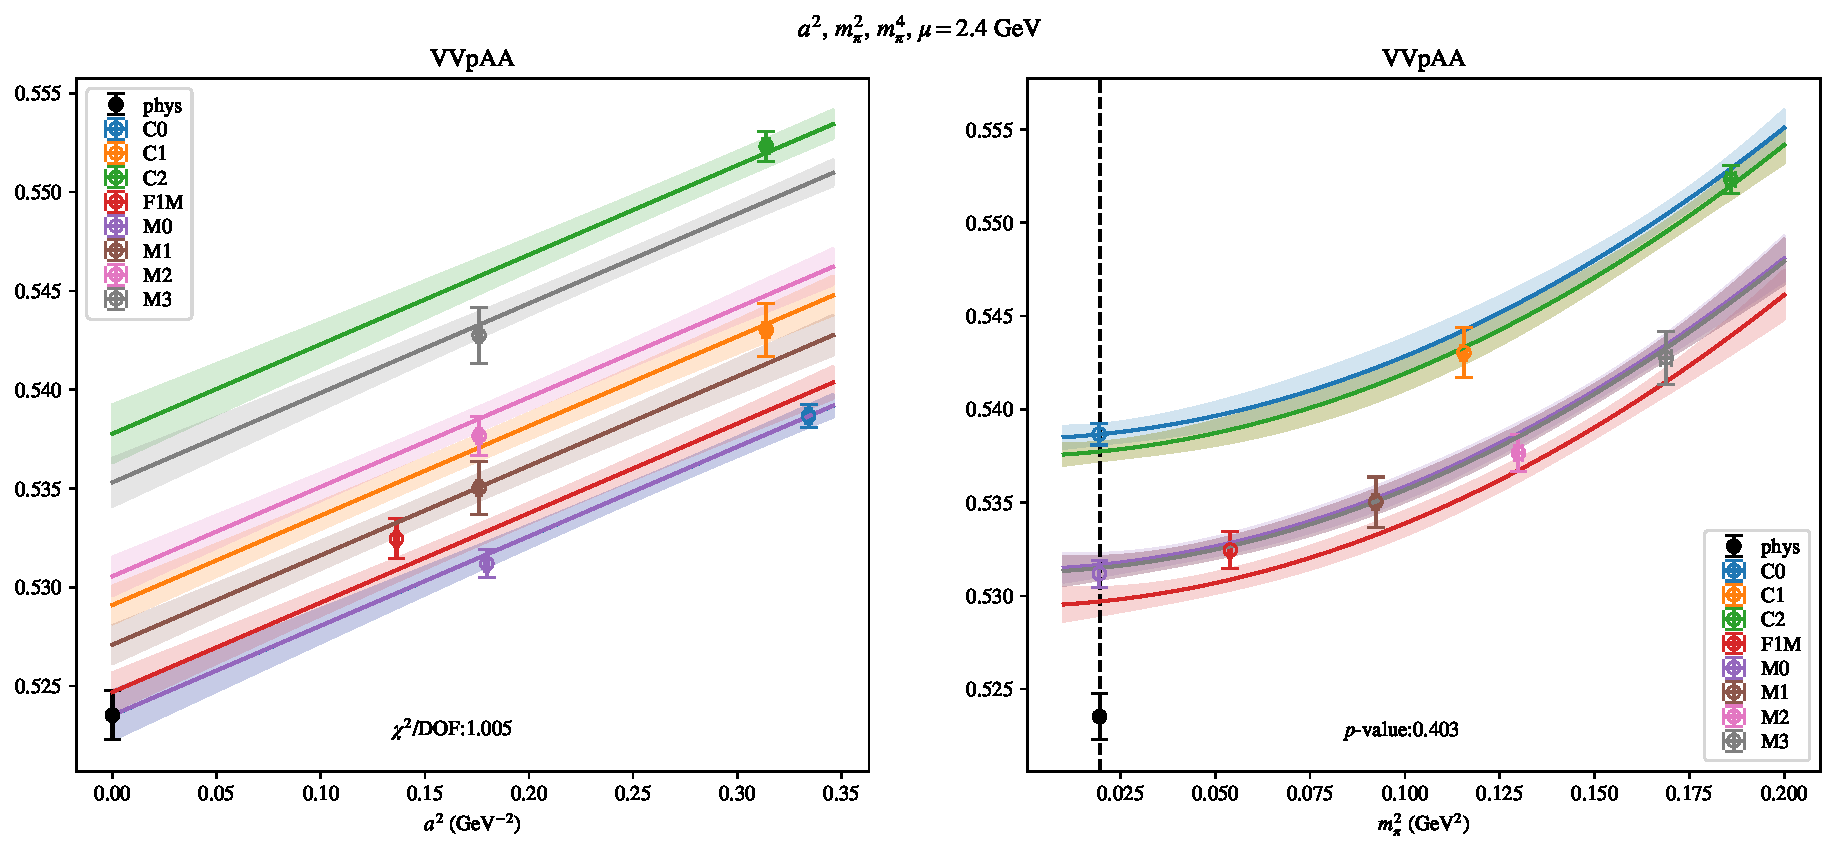
\includepdf[link, pages=-]{VVpAA/NPR/a2m2m4_24.pdf}
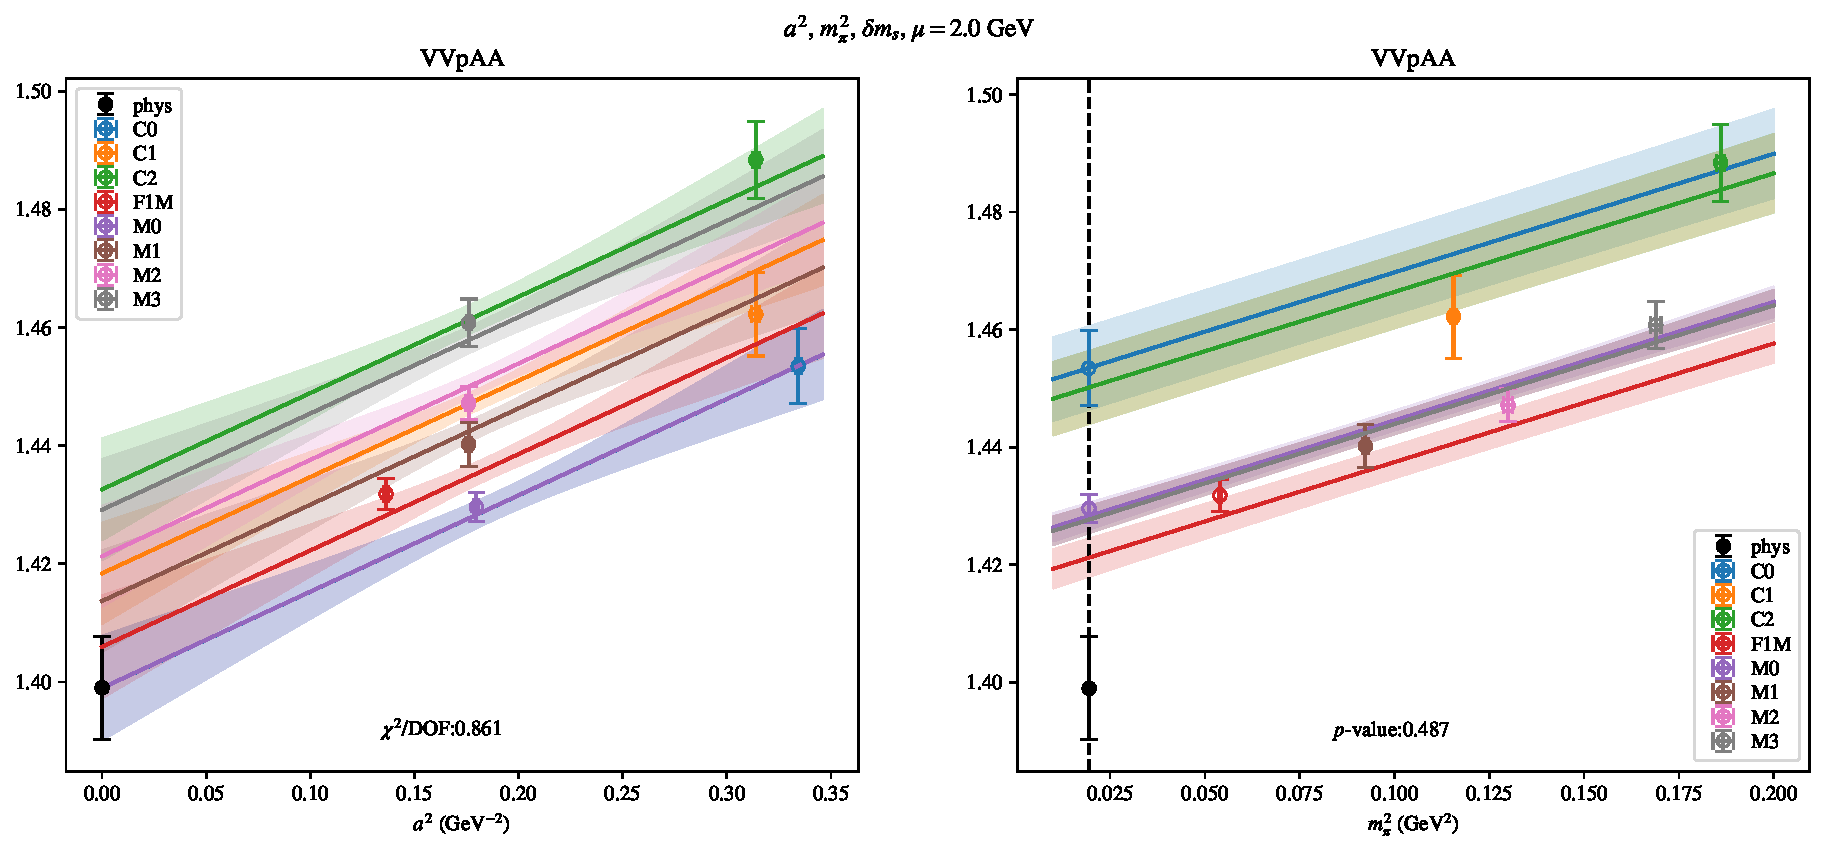
\includepdf[link, pages=-]{VVpAA/NPR/a2m2delm_20.pdf}
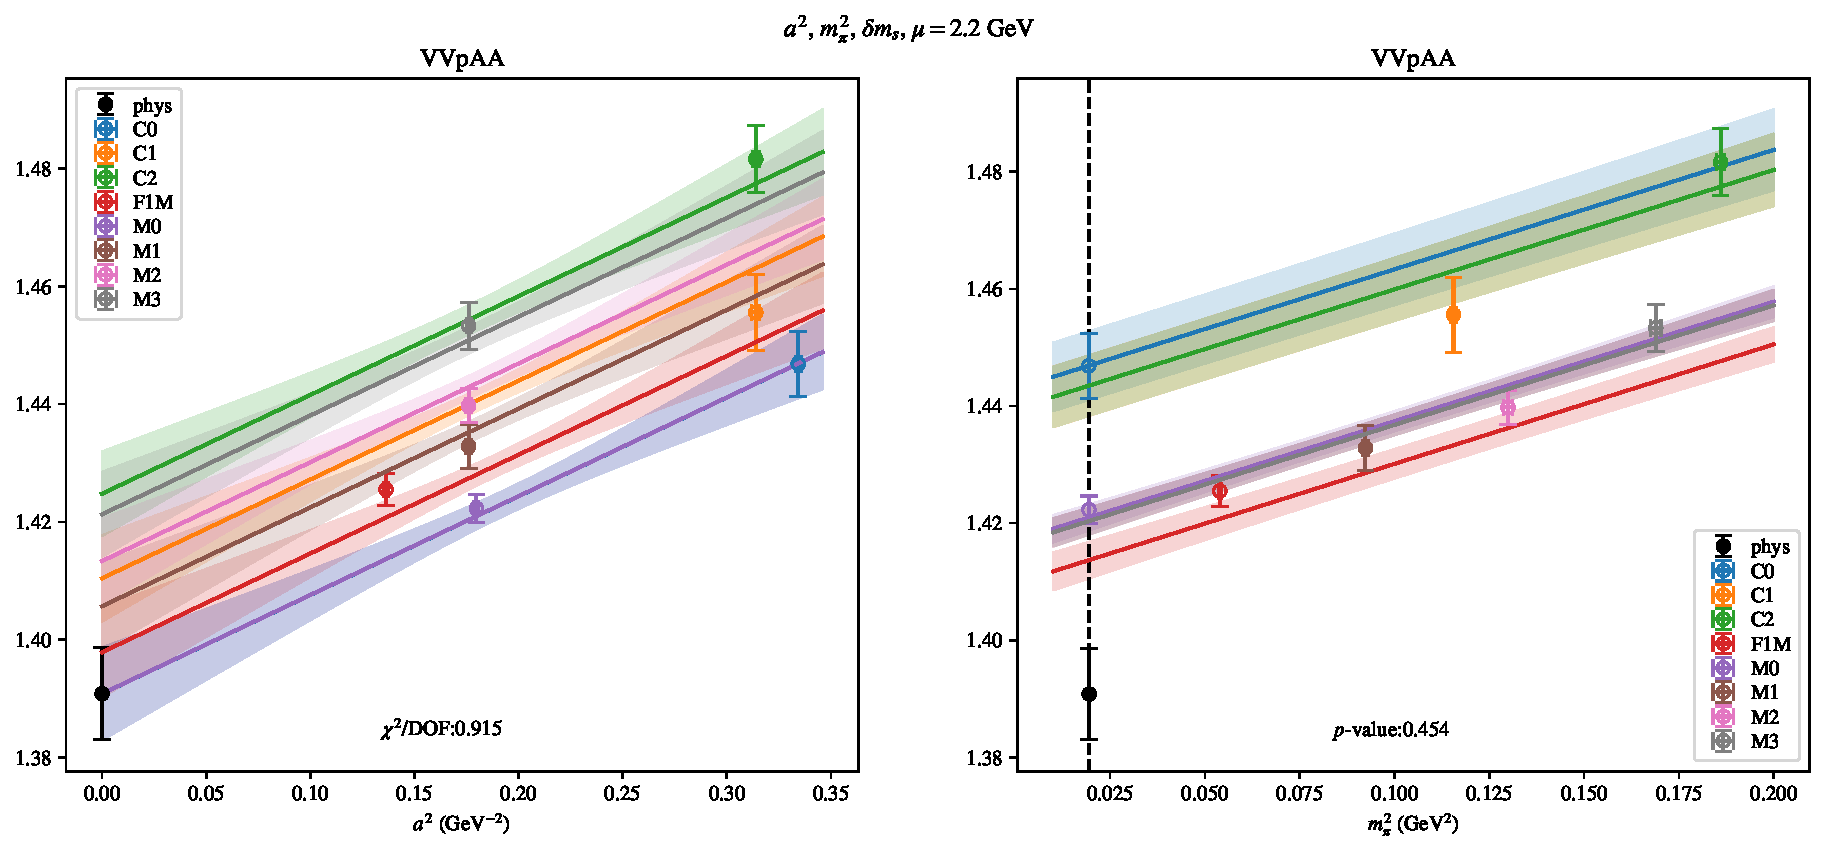
\includepdf[link, pages=-]{VVpAA/NPR/a2m2delm_22.pdf}
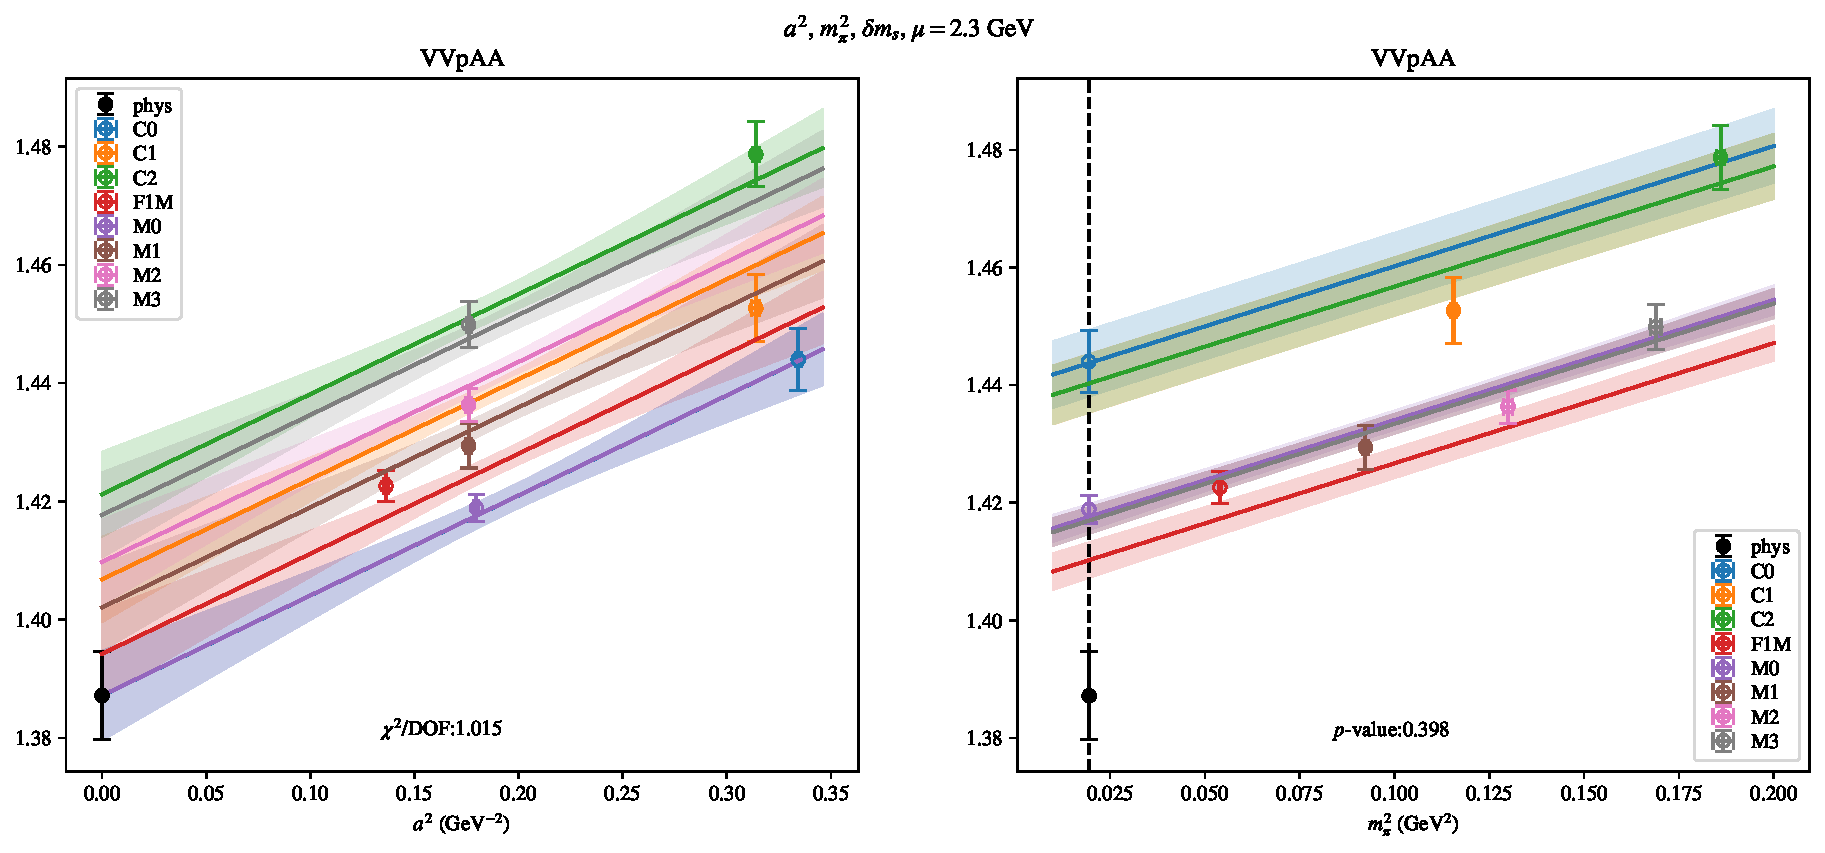
\includepdf[link, pages=-]{VVpAA/NPR/a2m2delm_23.pdf}
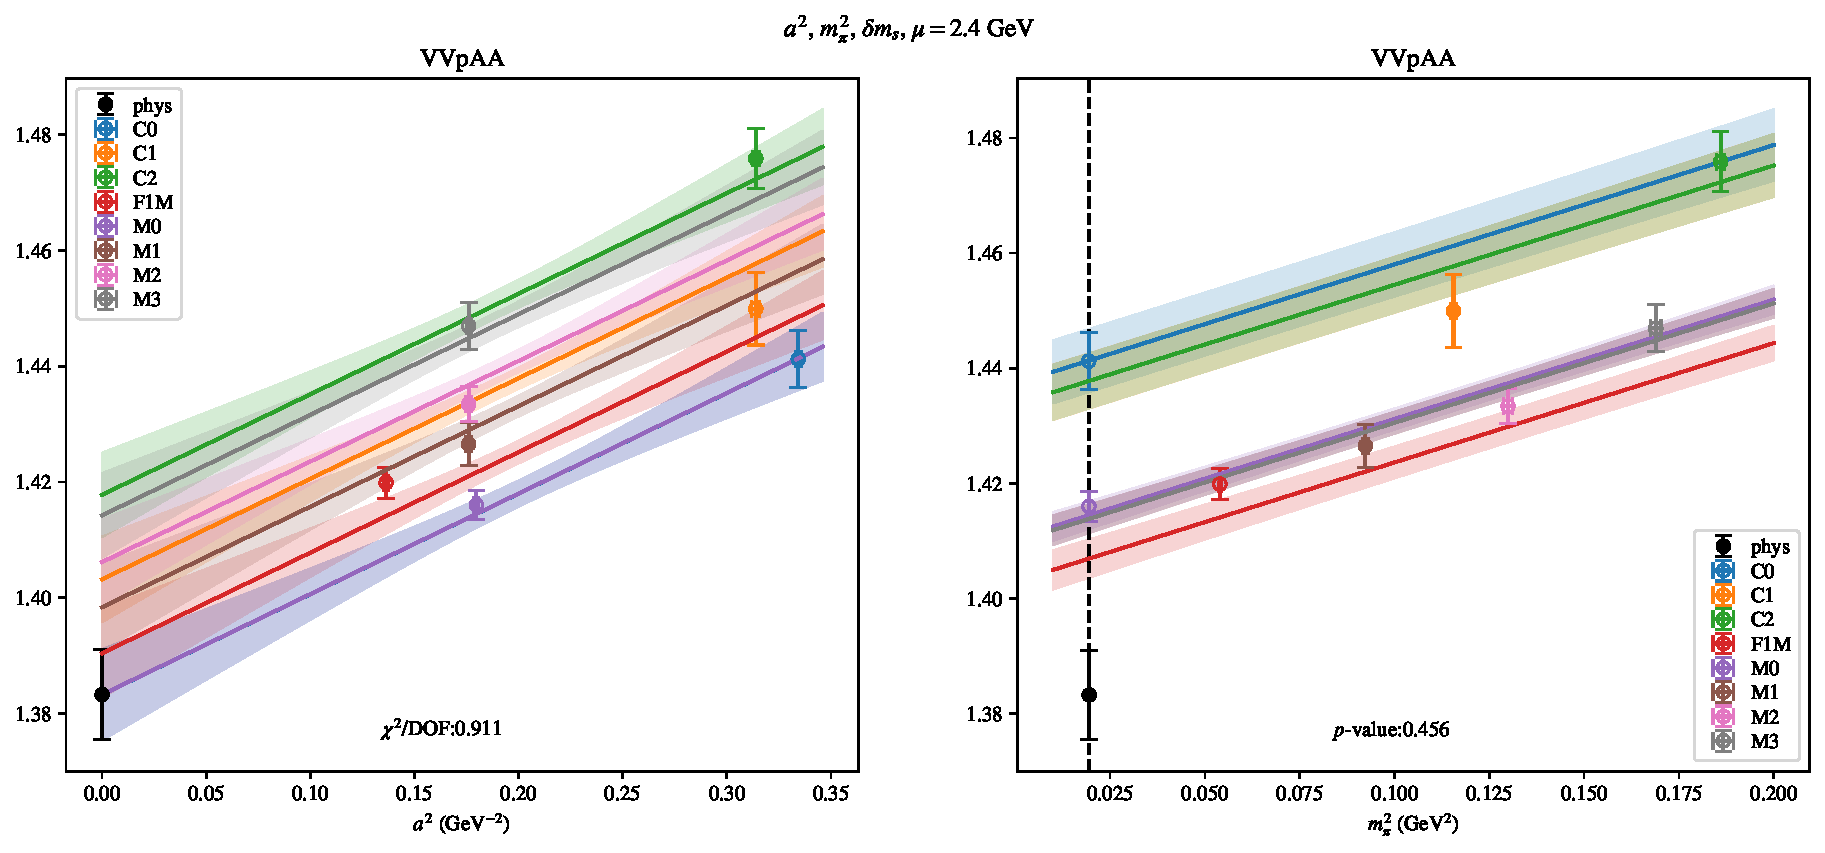
\includepdf[link, pages=-]{VVpAA/NPR/a2m2delm_24.pdf}
\clearpage
\section{$\mathcal{B}_2$}
\begin{table}[h!]
\begin{center}
\begin{tabular}{|c|c|c|c|c|c|c|}
\hline
$\mu$ (GeV) & $a^2$, $m_\pi^2$& $a^2$, $m_\pi^2$ (no C)& $a^2$, $m_\pi^2$, $a^4$& $a^2$, $m_\pi^2$ (no M3, C2)& $a^2$, $m_\pi^2$, $m_\pi^4$& $a^2$, $m_\pi^2$, $\delta m_s$\\
\hline
2.0& \hyperlink{VVmAA/NPR/a2m2_20.pdf.1}{\textbf{-0.992(15)}: 10.458 (0.0)} & \hyperlink{VVmAA/NPR/a2m2noC_20.pdf.1}{\textbf{-0.933(98)}: 1.858 (0.156)} & \hyperlink{VVmAA/NPR/a2a4m2_20.pdf.1}{\textbf{-0.89(12)}: 1.832 (0.12)} & \hyperlink{VVmAA/NPR/a2m2mcut_20.pdf.1}{\textbf{-0.993(21)}: 16.356 (0.0)} & \hyperlink{VVmAA/NPR/a2m2m4_20.pdf.1}{\textbf{-0.994(16)}: 10.015 (0.0)} & \hyperlink{VVmAA/NPR/a2m2delm_20.pdf.1}{\textbf{-0.994(15)}: 2.064 (0.083)}\\
2.2& \hyperlink{VVmAA/NPR/a2m2_22.pdf.1}{\textbf{-1.006(15)}: 10.04 (0.0)} & \hyperlink{VVmAA/NPR/a2m2noC_22.pdf.1}{\textbf{-0.952(97)}: 2.909 (0.055)} & \hyperlink{VVmAA/NPR/a2a4m2_22.pdf.1}{\textbf{-0.91(13)}: 2.564 (0.036)} & \hyperlink{VVmAA/NPR/a2m2mcut_22.pdf.1}{\textbf{-1.008(21)}: 14.196 (0.0)} & \hyperlink{VVmAA/NPR/a2m2m4_22.pdf.1}{\textbf{-1.009(17)}: 8.526 (0.0)} & \hyperlink{VVmAA/NPR/a2m2delm_22.pdf.1}{\textbf{-1.008(15)}: 3.189 (0.013)}\\
2.3& \hyperlink{VVmAA/NPR/a2m2_23.pdf.1}{\textbf{-1.012(14)}: 10.124 (0.0)} & \hyperlink{VVmAA/NPR/a2m2noC_23.pdf.1}{\textbf{-0.958(94)}: 3.107 (0.045)} & \hyperlink{VVmAA/NPR/a2a4m2_23.pdf.1}{\textbf{-0.92(13)}: 2.443 (0.044)} & \hyperlink{VVmAA/NPR/a2m2mcut_23.pdf.1}{\textbf{-1.014(21)}: 14.517 (0.0)} & \hyperlink{VVmAA/NPR/a2m2m4_23.pdf.1}{\textbf{-1.015(16)}: 8.92 (0.0)} & \hyperlink{VVmAA/NPR/a2m2delm_23.pdf.1}{\textbf{-1.014(14)}: 3.229 (0.012)}\\
2.4& \hyperlink{VVmAA/NPR/a2m2_24.pdf.1}{\textbf{-1.017(14)}: 9.337 (0.0)} & \hyperlink{VVmAA/NPR/a2m2noC_24.pdf.1}{\textbf{-0.965(91)}: 3.1 (0.045)} & \hyperlink{VVmAA/NPR/a2a4m2_24.pdf.1}{\textbf{-0.93(12)}: 2.634 (0.032)} & \hyperlink{VVmAA/NPR/a2m2mcut_24.pdf.1}{\textbf{-1.019(20)}: 13.254 (0.0)} & \hyperlink{VVmAA/NPR/a2m2m4_24.pdf.1}{\textbf{-1.019(16)}: 8.327 (0.0)} & \hyperlink{VVmAA/NPR/a2m2delm_24.pdf.1}{\textbf{-1.019(14)}: 3.035 (0.016)}\\
\hline
\end{tabular}
\caption{Physical point value from chiral and continuum extrapolation at renormalisation scale $\mu$. Entries are \textbf{value(error)}: $\chi^2/\text{DOF}$ ($p$-value).}
\end{center}
\end{table}
\begin{table}[h!]
\begin{center}
\begin{tabular}{|c c|c|c|c|c|c|c|}
\hline
$\mu$ (GeV) &  & $a^2$, $m_\pi^2$& $a^2$, $m_\pi^2$ (no C)& $a^2$, $m_\pi^2$, $a^4$& $a^2$, $m_\pi^2$ (no M3, C2)& $a^2$, $m_\pi^2$, $m_\pi^4$& $a^2$, $m_\pi^2$, $\delta m_s$\\
\hline
\multirow{3}{0.5in}{2.0} & $\alpha$ & -0.187(60)& 0.164(61)& 0.79(13)& -0.193(88)& -0.194(67)& -0.197(60)\\
 & $\beta$ & 0.00107(14)& 0.00080(43)& 0.00090(16)& 0.00057(29)& -0.0020(90)& 0.00075(15)\\
 & $\gamma$ &  &  & -2.0(28)&  & 0.000284(81)& 0.0147(21)\\
\hline
\multirow{3}{0.5in}{2.2} & $\alpha$ & -0.229(62)& 0.087(59)& 0.63(13)& -0.234(90)& -0.236(70)& -0.237(60)\\
 & $\beta$ & 0.00121(12)& 0.00099(31)& 0.00106(14)& 0.00058(25)& -0.0019(82)& 0.00093(13)\\
 & $\gamma$ &  &  & -1.7(28)&  & 0.000285(75)& 0.0128(21)\\
\hline
\multirow{3}{0.5in}{2.3} & $\alpha$ & -0.251(60)& 0.061(56)& 0.61(13)& -0.256(87)& -0.258(68)& -0.259(58)\\
 & $\beta$ & 0.00122(12)& 0.00100(29)& 0.00107(14)& 0.00063(24)& -0.0017(79)& 0.00093(13)\\
 & $\gamma$ &  &  & -1.7(27)&  & 0.000269(72)& 0.0126(20)\\
\hline
\multirow{3}{0.5in}{2.4} & $\alpha$ & -0.270(56)& 0.025(53)& 0.53(12)& -0.275(84)& -0.277(65)& -0.277(55)\\
 & $\beta$ & 0.00118(12)& 0.00099(29)& 0.00103(13)& 0.00062(23)& -0.0016(78)& 0.00091(13)\\
 & $\gamma$ &  &  & -1.6(26)&  & 0.000254(72)& 0.0119(20)\\
\hline
\end{tabular}
\caption{Fit values of coefficients in $Q = Q_{phys} + \mathbf{\alpha} a^2 + \mathbf{\beta}\left(\frac{m_\pi^2}{f_\pi^2}-\frac{m_{\pi,PDG}^2}{f_\pi^2}\right) + \gamma(\ldots)$}
\end{center}
\end{table}
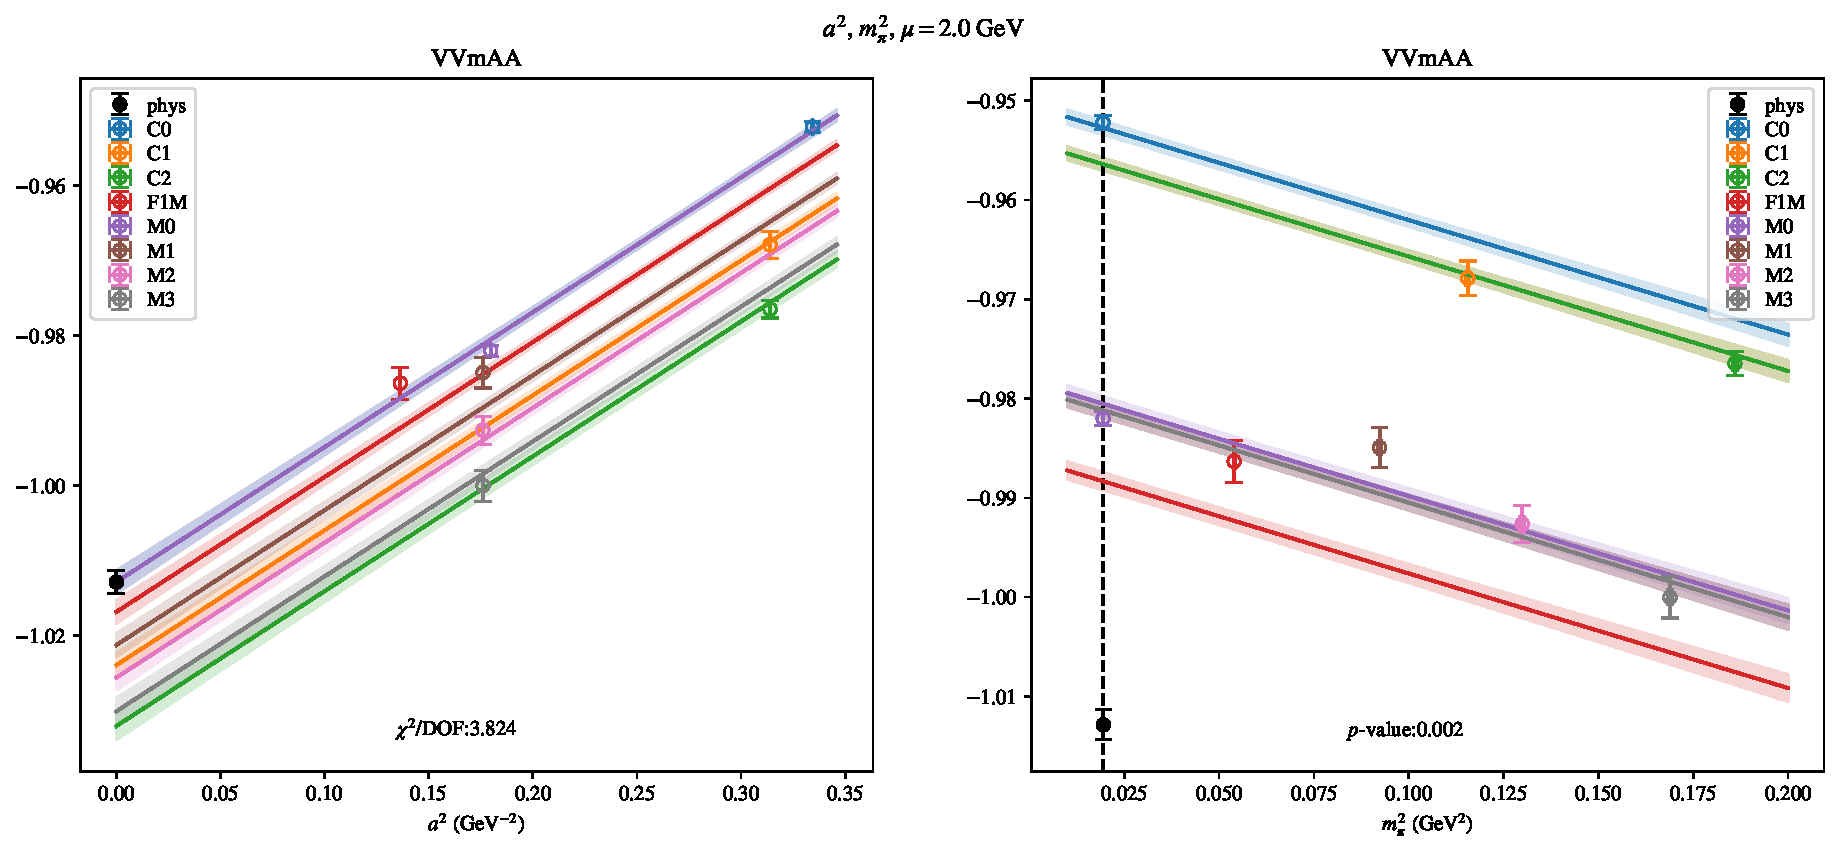
\includepdf[link, pages=-]{VVmAA/NPR/a2m2_20.pdf}
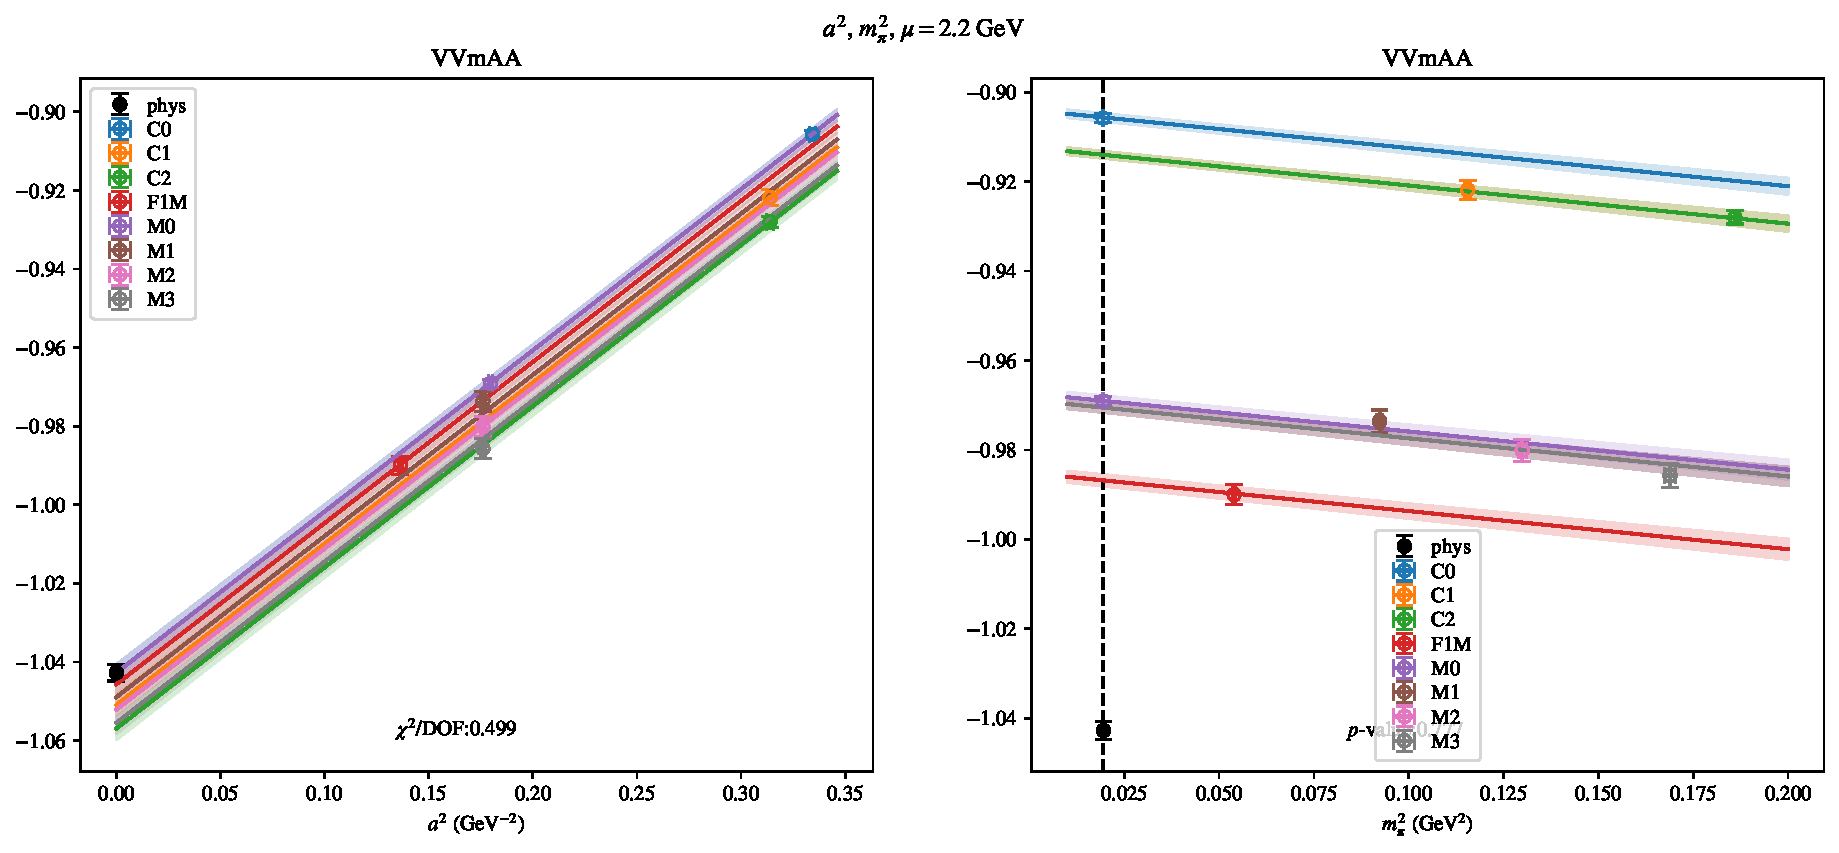
\includepdf[link, pages=-]{VVmAA/NPR/a2m2_22.pdf}
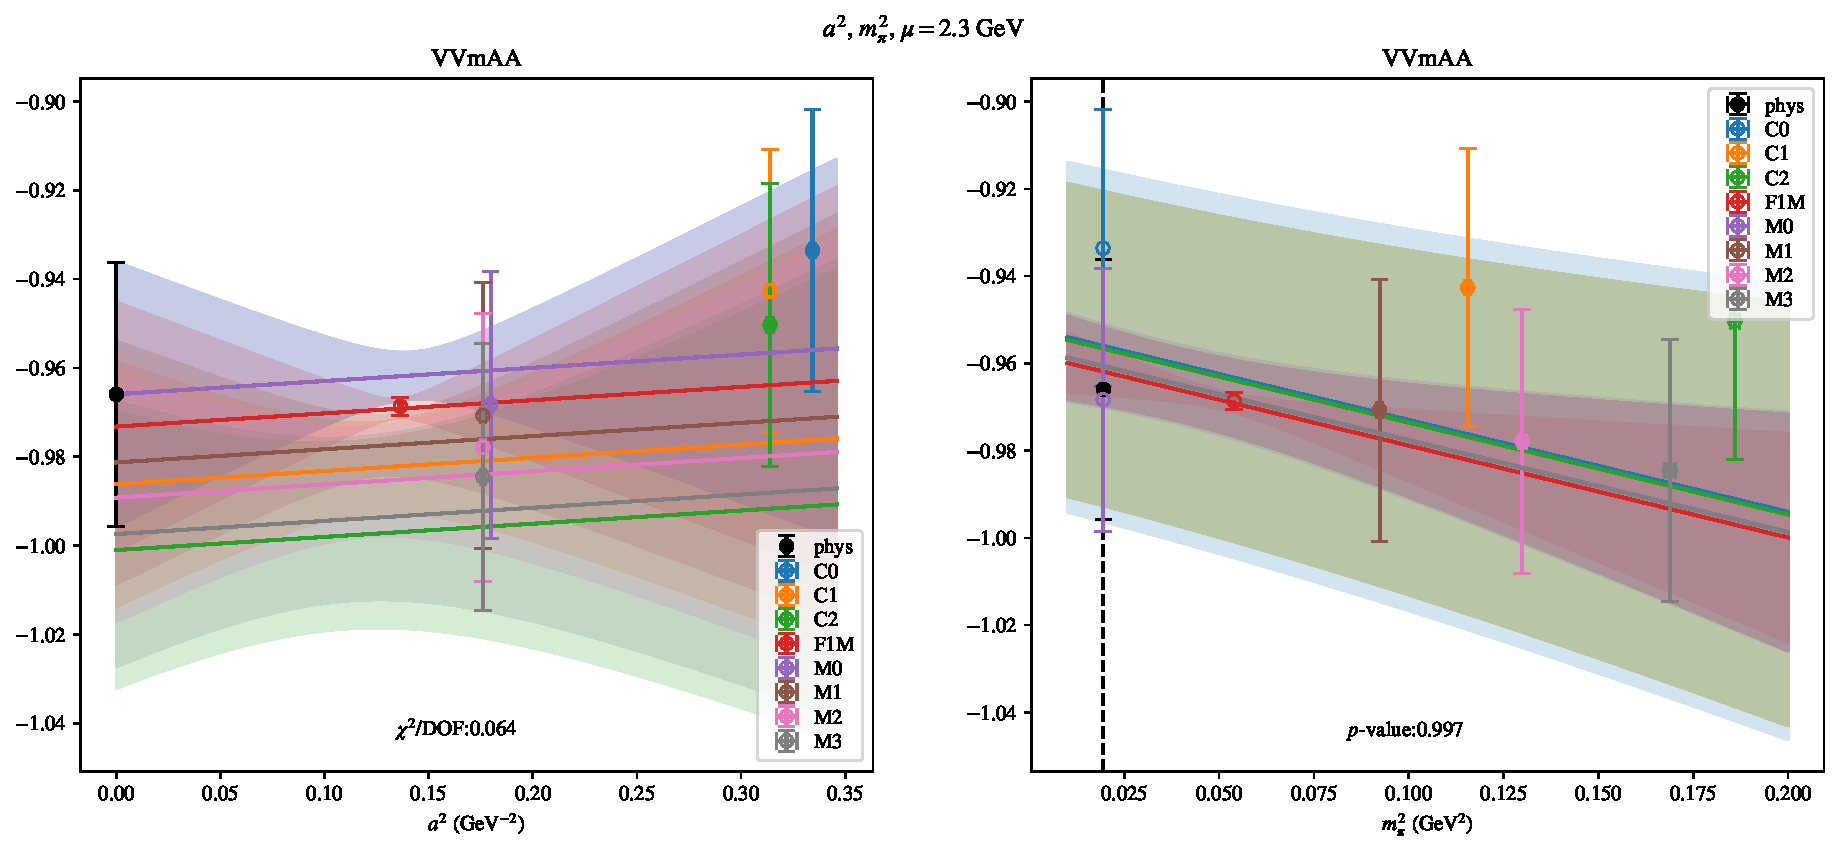
\includepdf[link, pages=-]{VVmAA/NPR/a2m2_23.pdf}
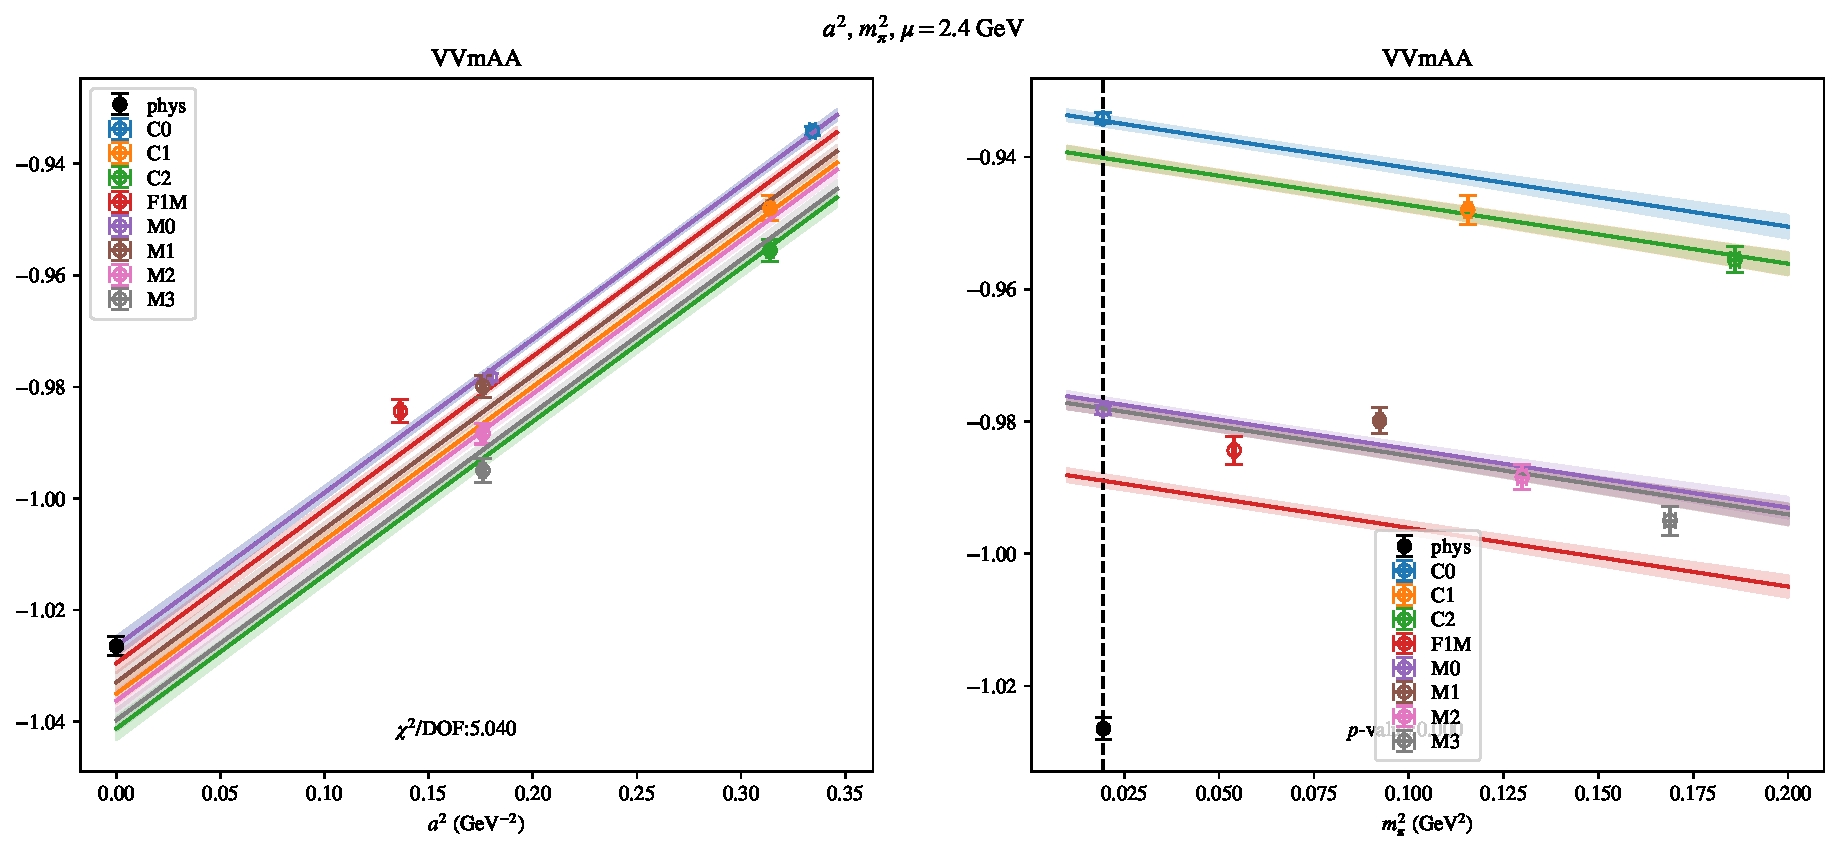
\includepdf[link, pages=-]{VVmAA/NPR/a2m2_24.pdf}
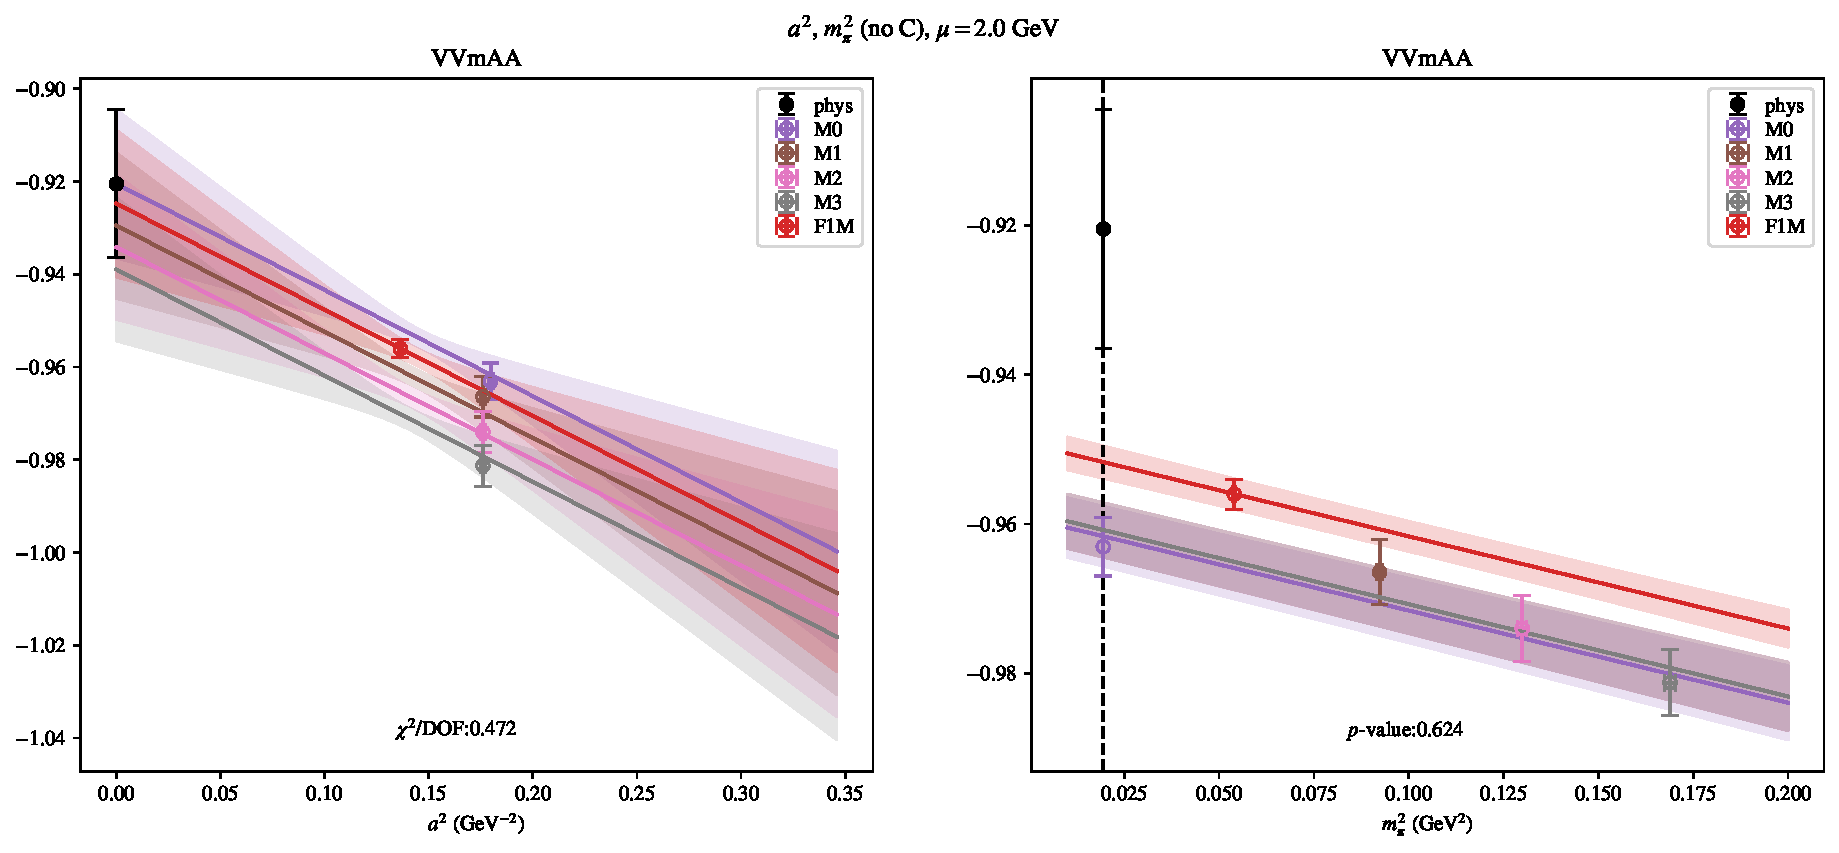
\includepdf[link, pages=-]{VVmAA/NPR/a2m2noC_20.pdf}
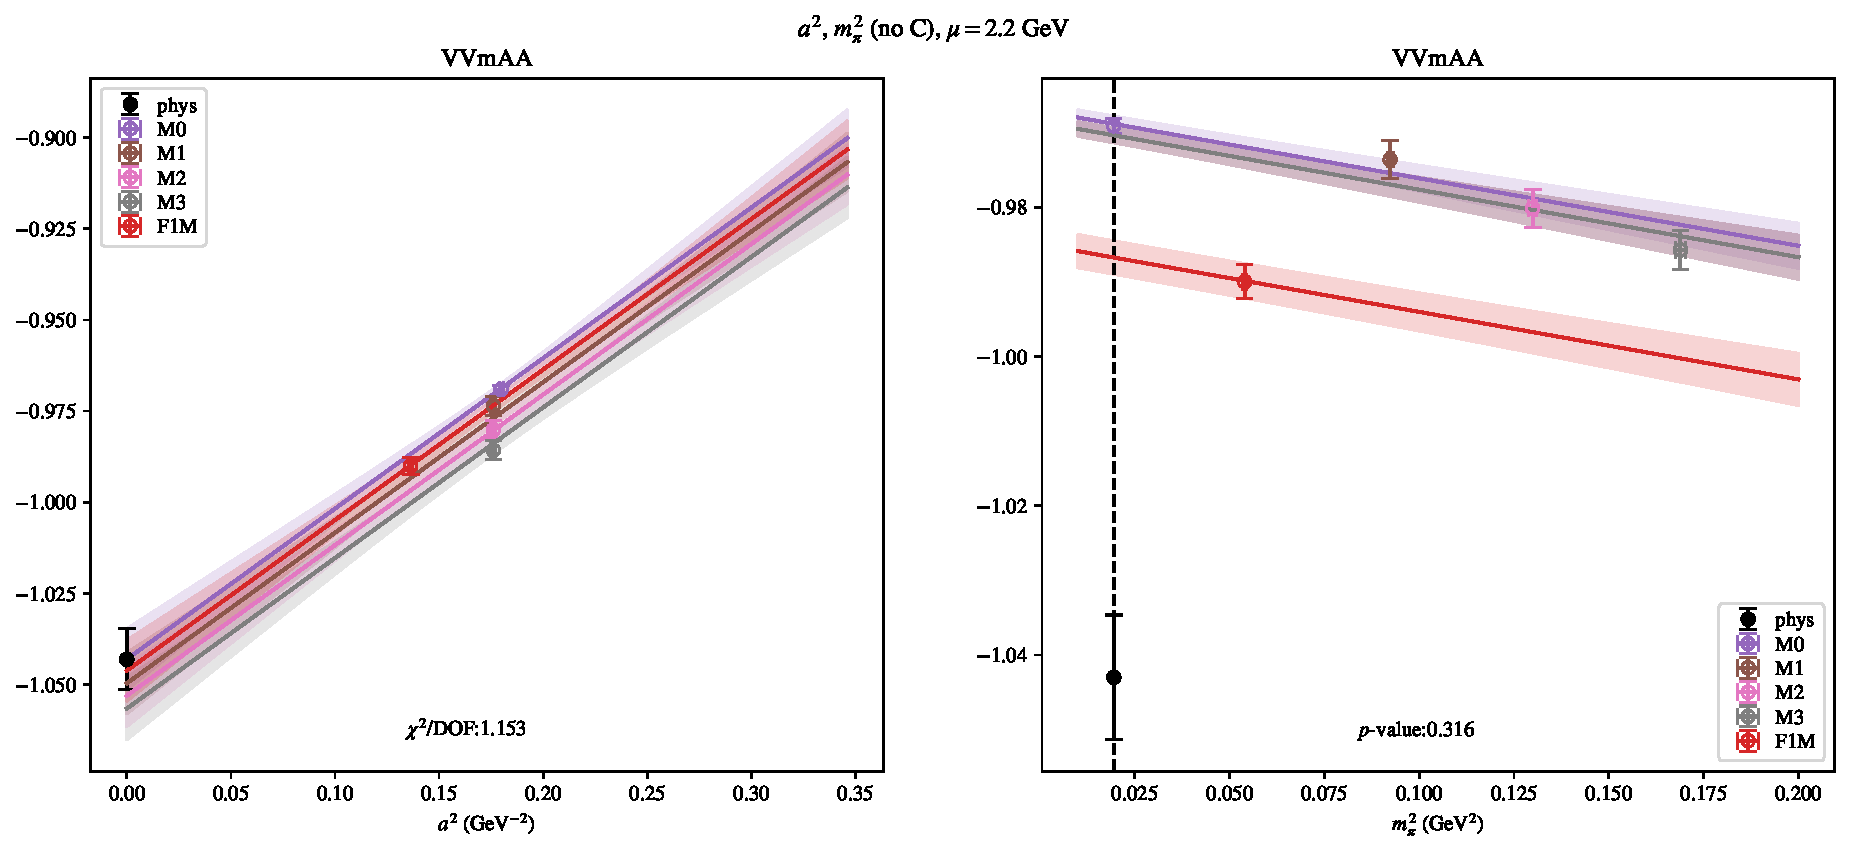
\includepdf[link, pages=-]{VVmAA/NPR/a2m2noC_22.pdf}
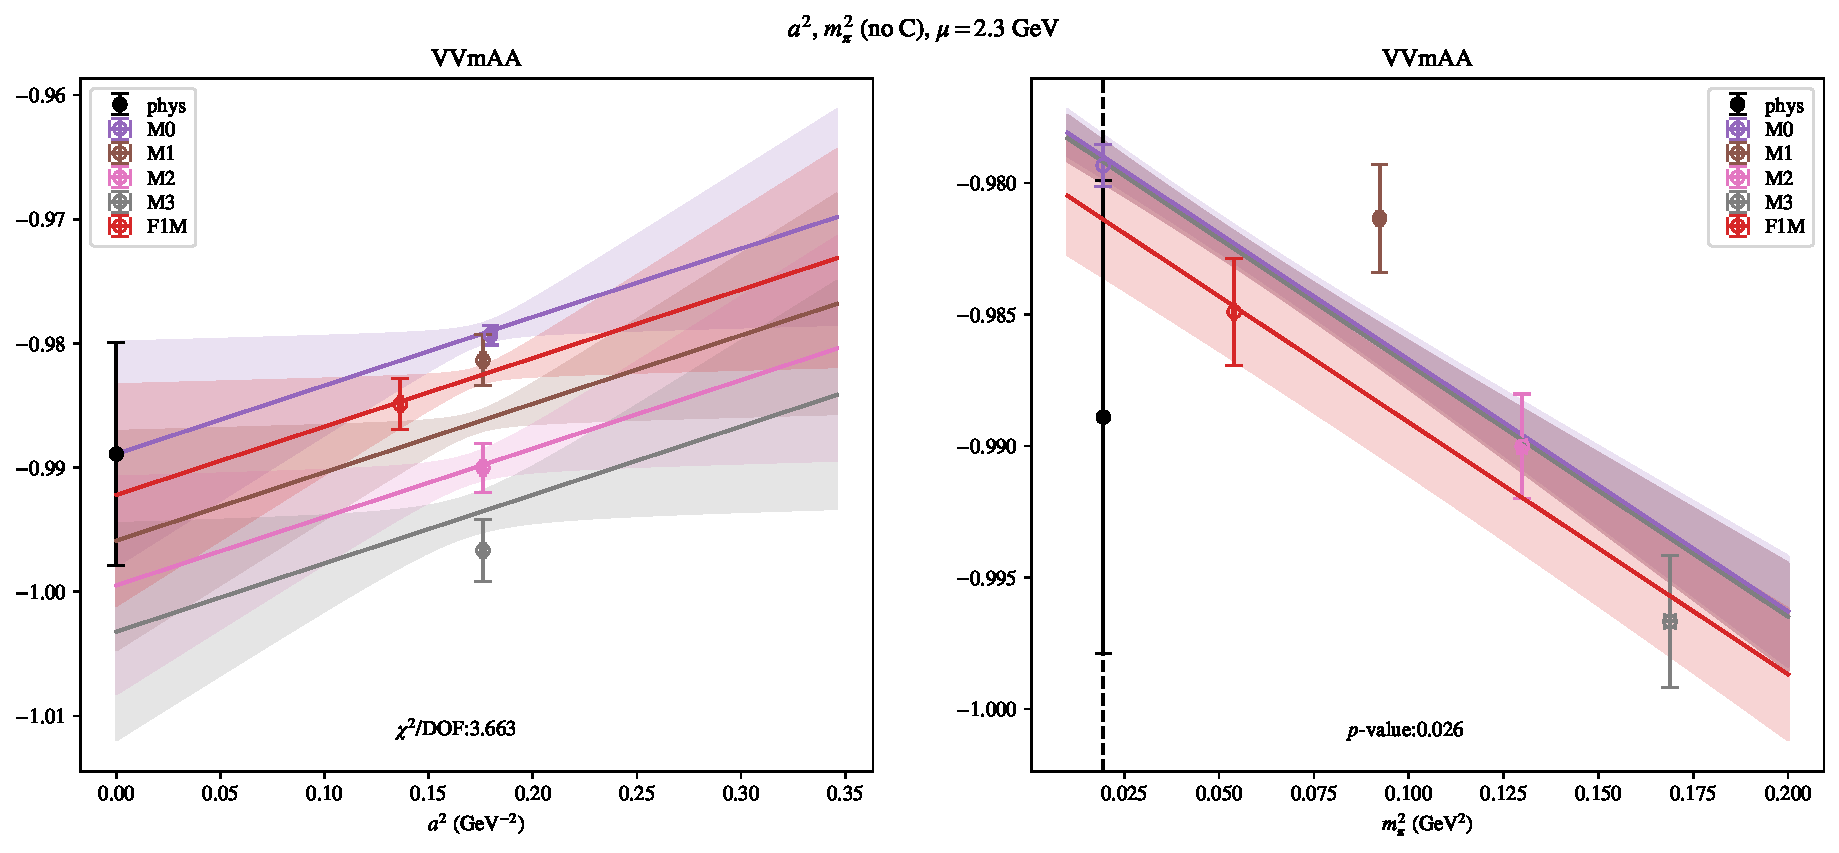
\includepdf[link, pages=-]{VVmAA/NPR/a2m2noC_23.pdf}
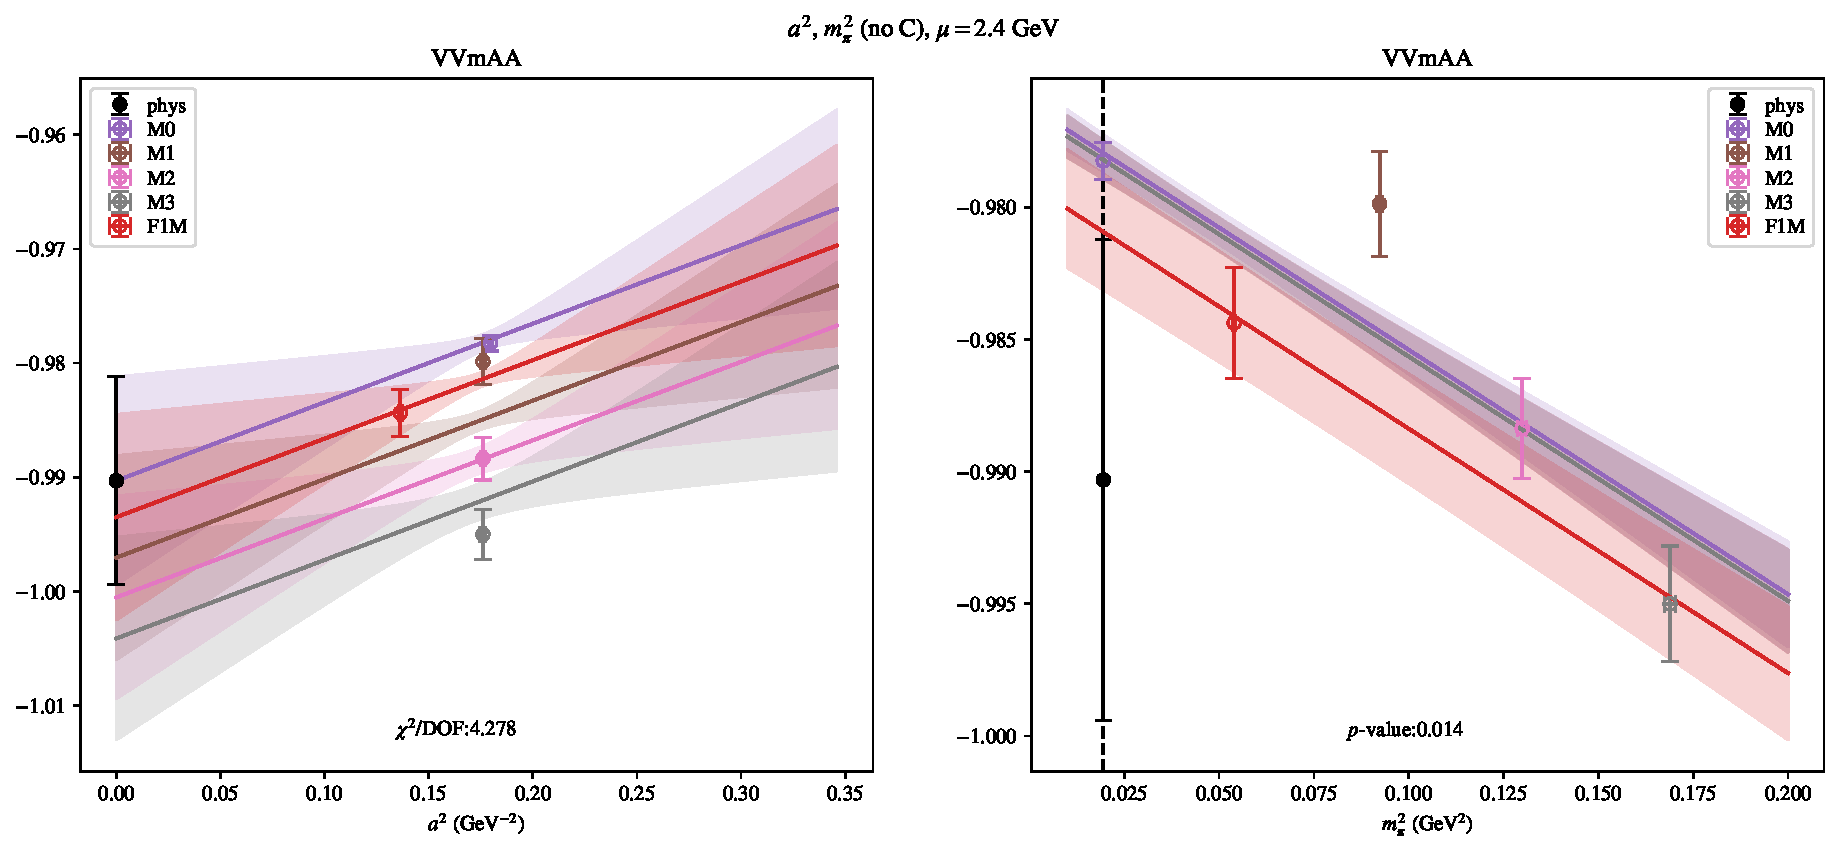
\includepdf[link, pages=-]{VVmAA/NPR/a2m2noC_24.pdf}
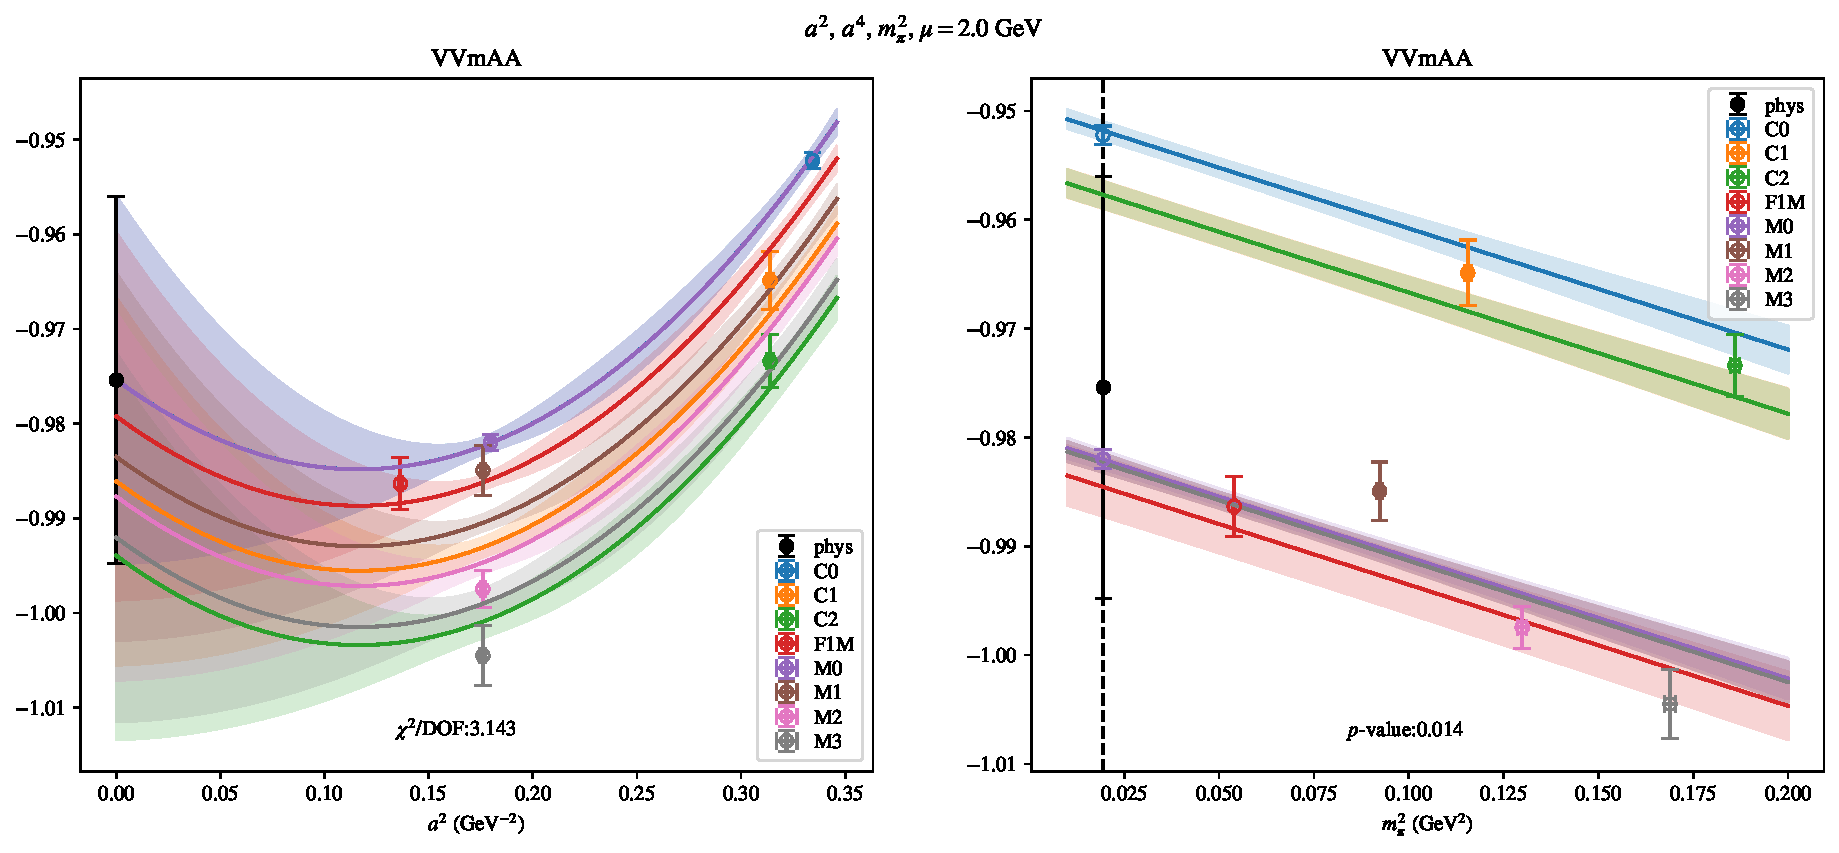
\includepdf[link, pages=-]{VVmAA/NPR/a2a4m2_20.pdf}
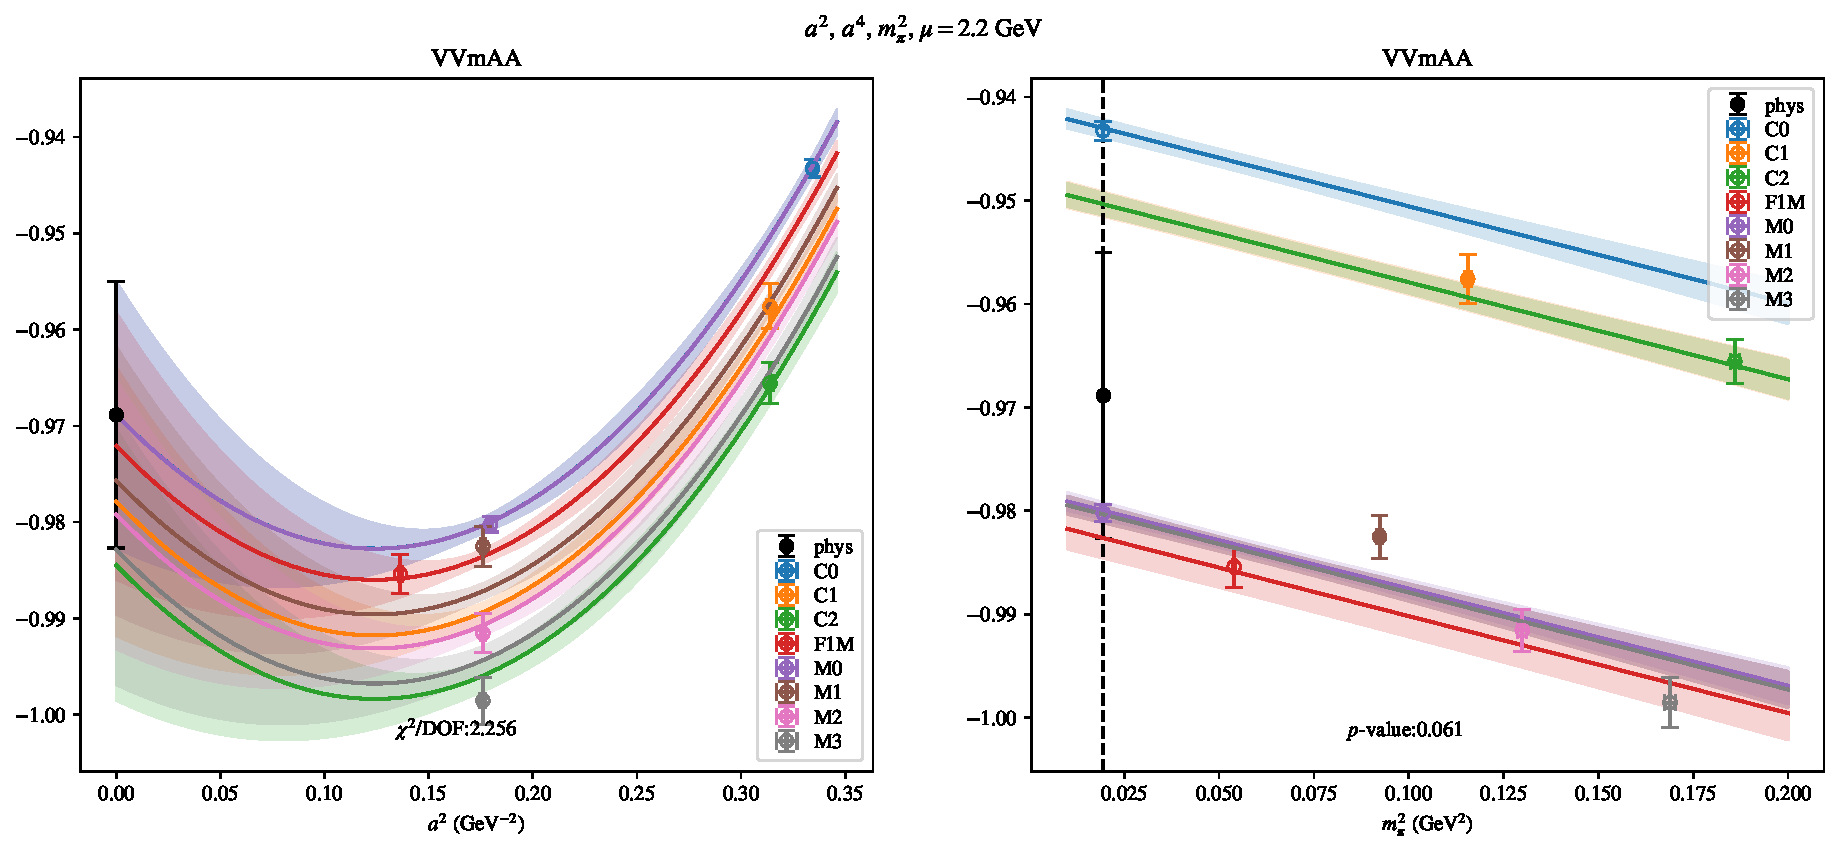
\includepdf[link, pages=-]{VVmAA/NPR/a2a4m2_22.pdf}
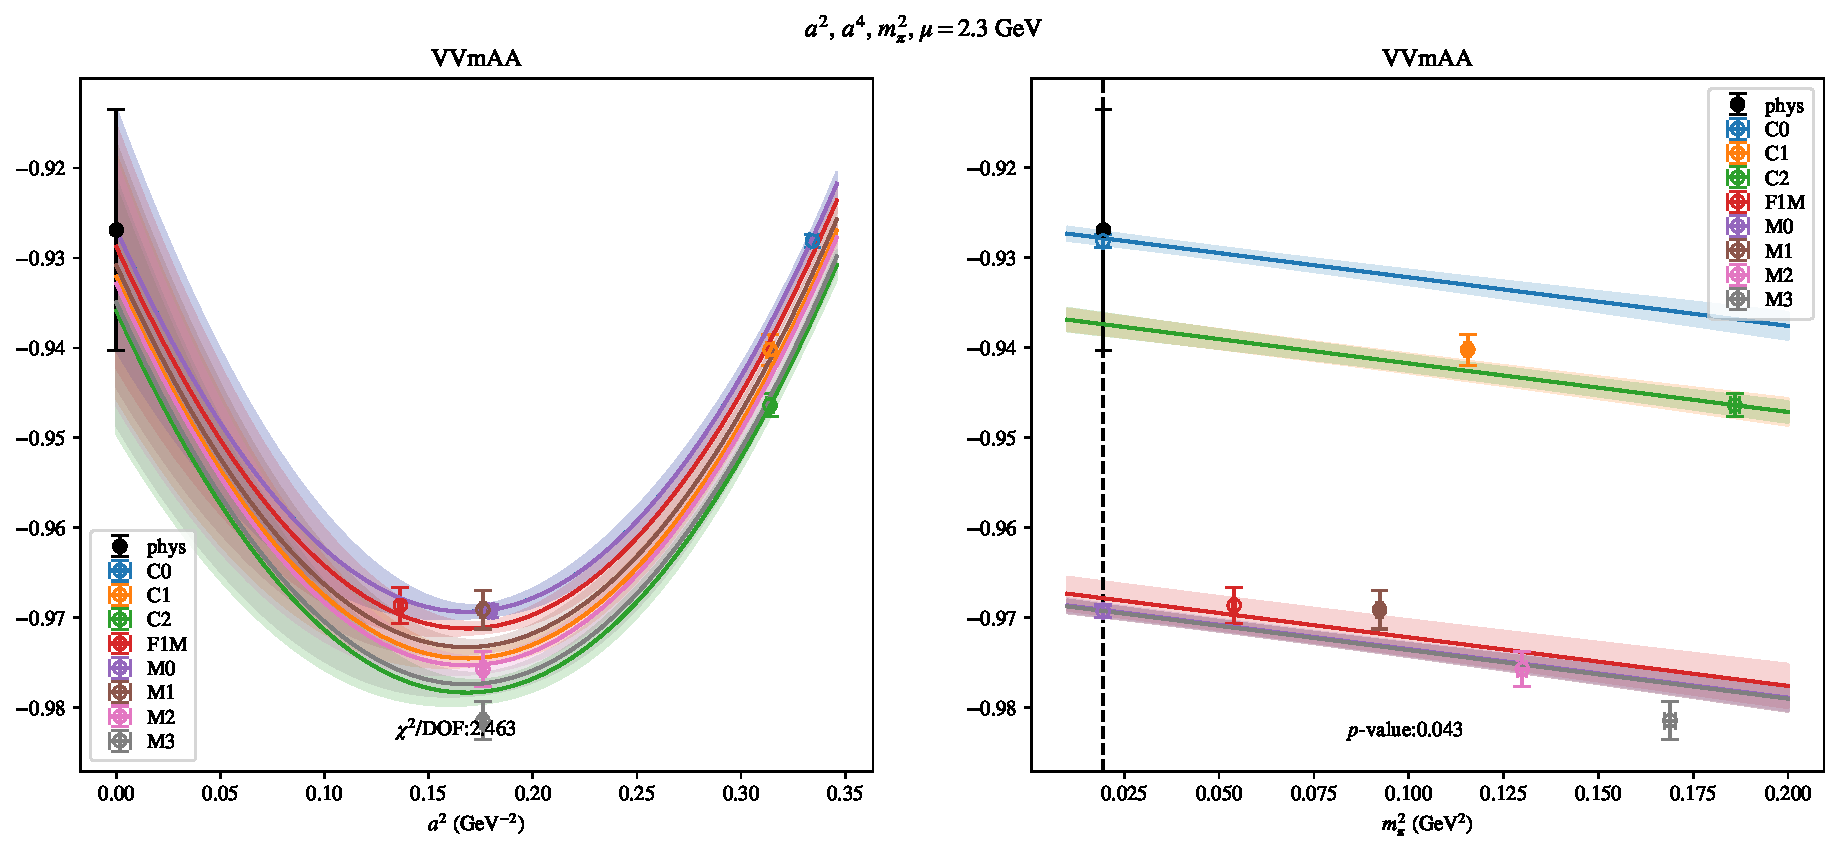
\includepdf[link, pages=-]{VVmAA/NPR/a2a4m2_23.pdf}
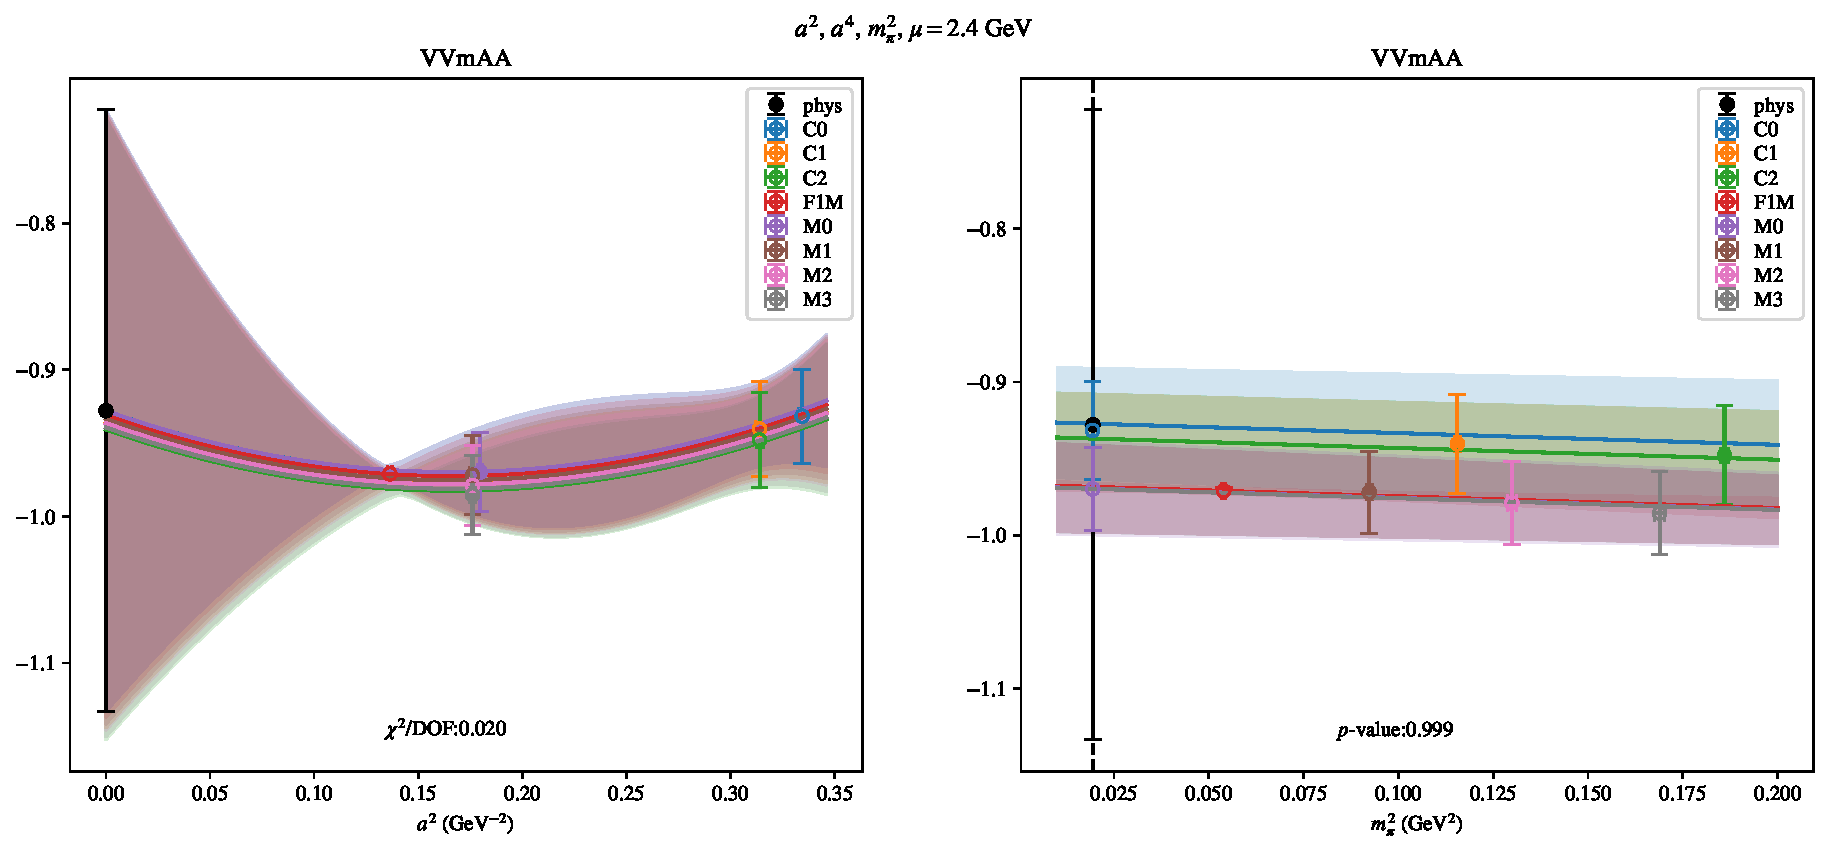
\includepdf[link, pages=-]{VVmAA/NPR/a2a4m2_24.pdf}
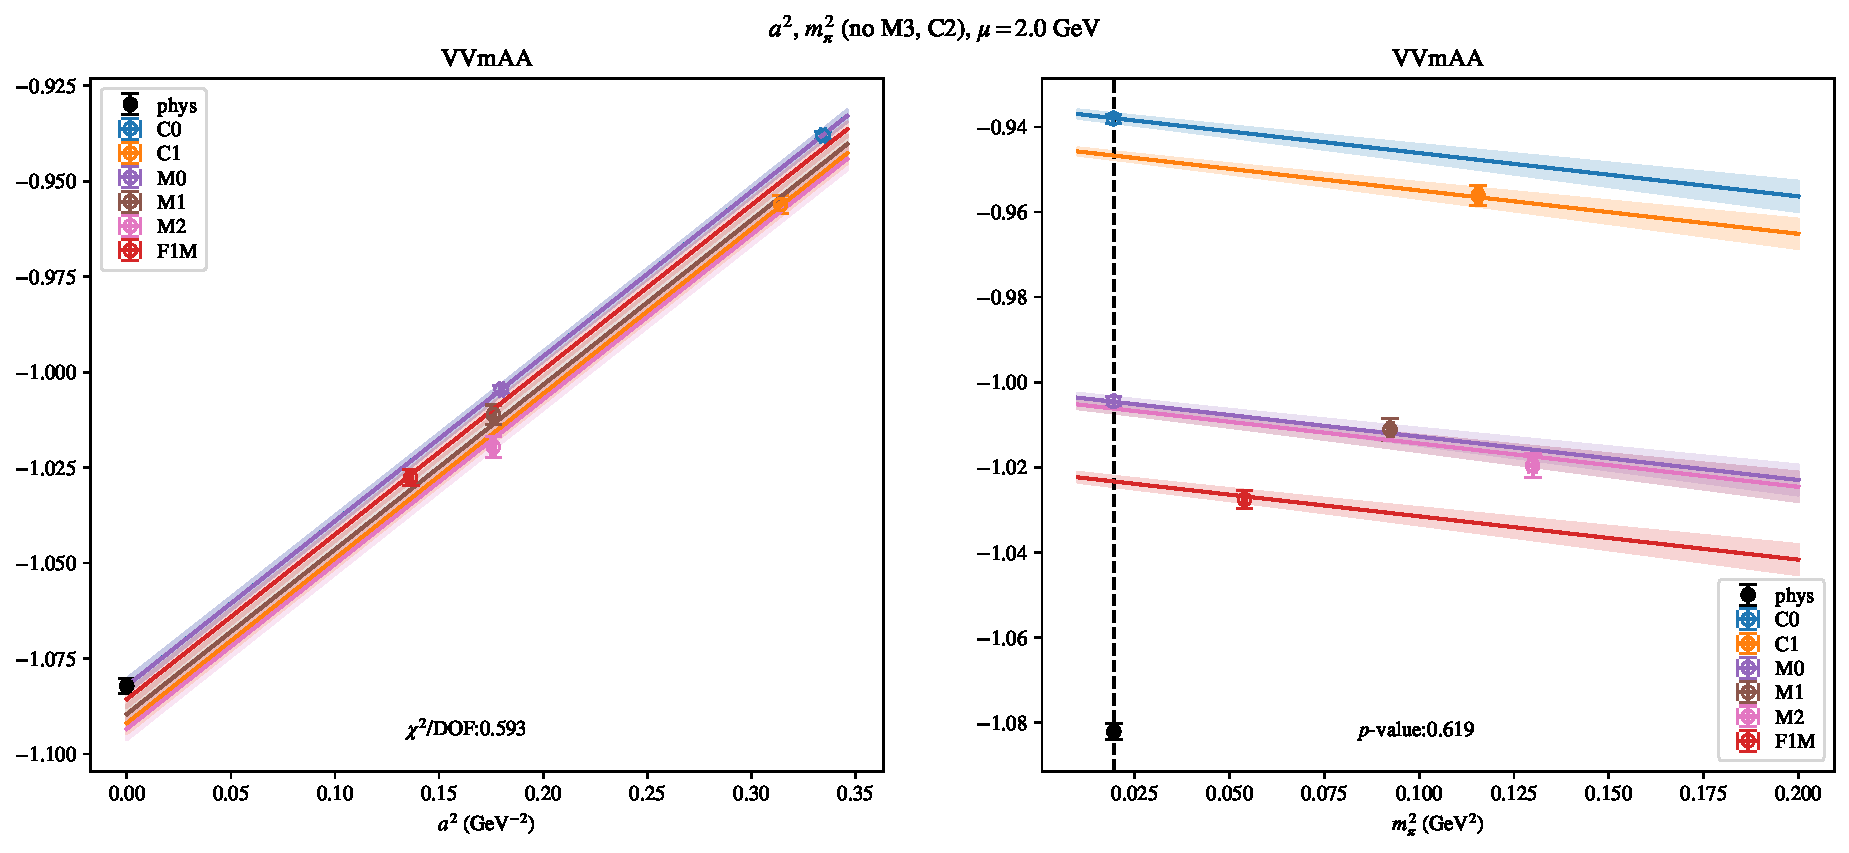
\includepdf[link, pages=-]{VVmAA/NPR/a2m2mcut_20.pdf}
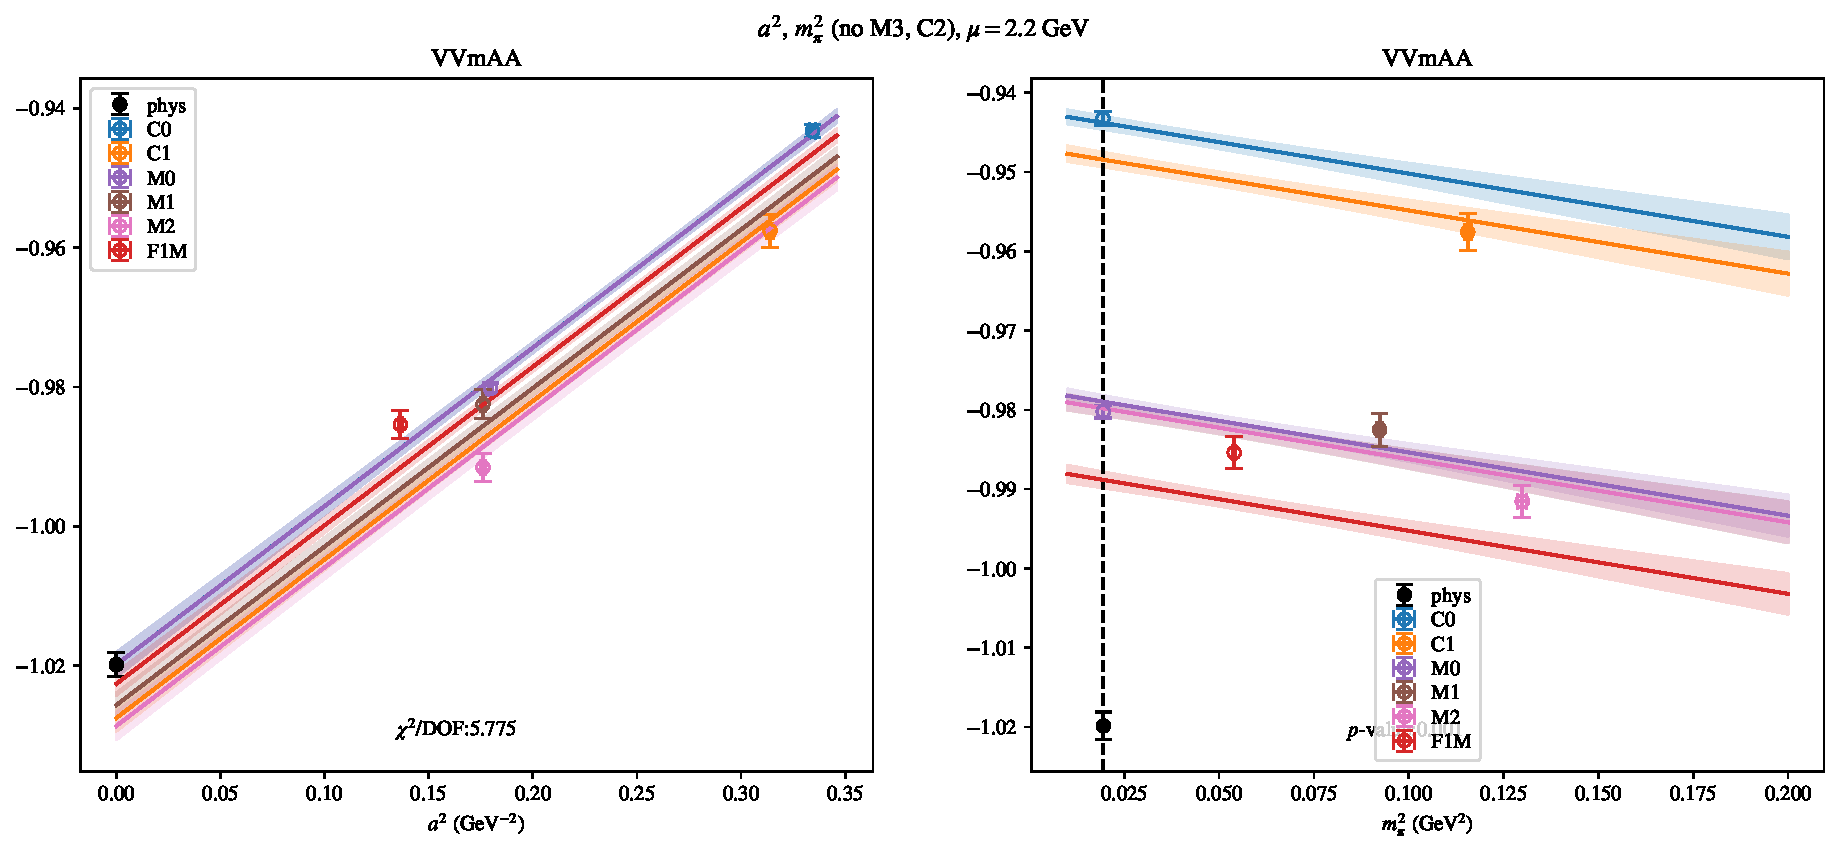
\includepdf[link, pages=-]{VVmAA/NPR/a2m2mcut_22.pdf}
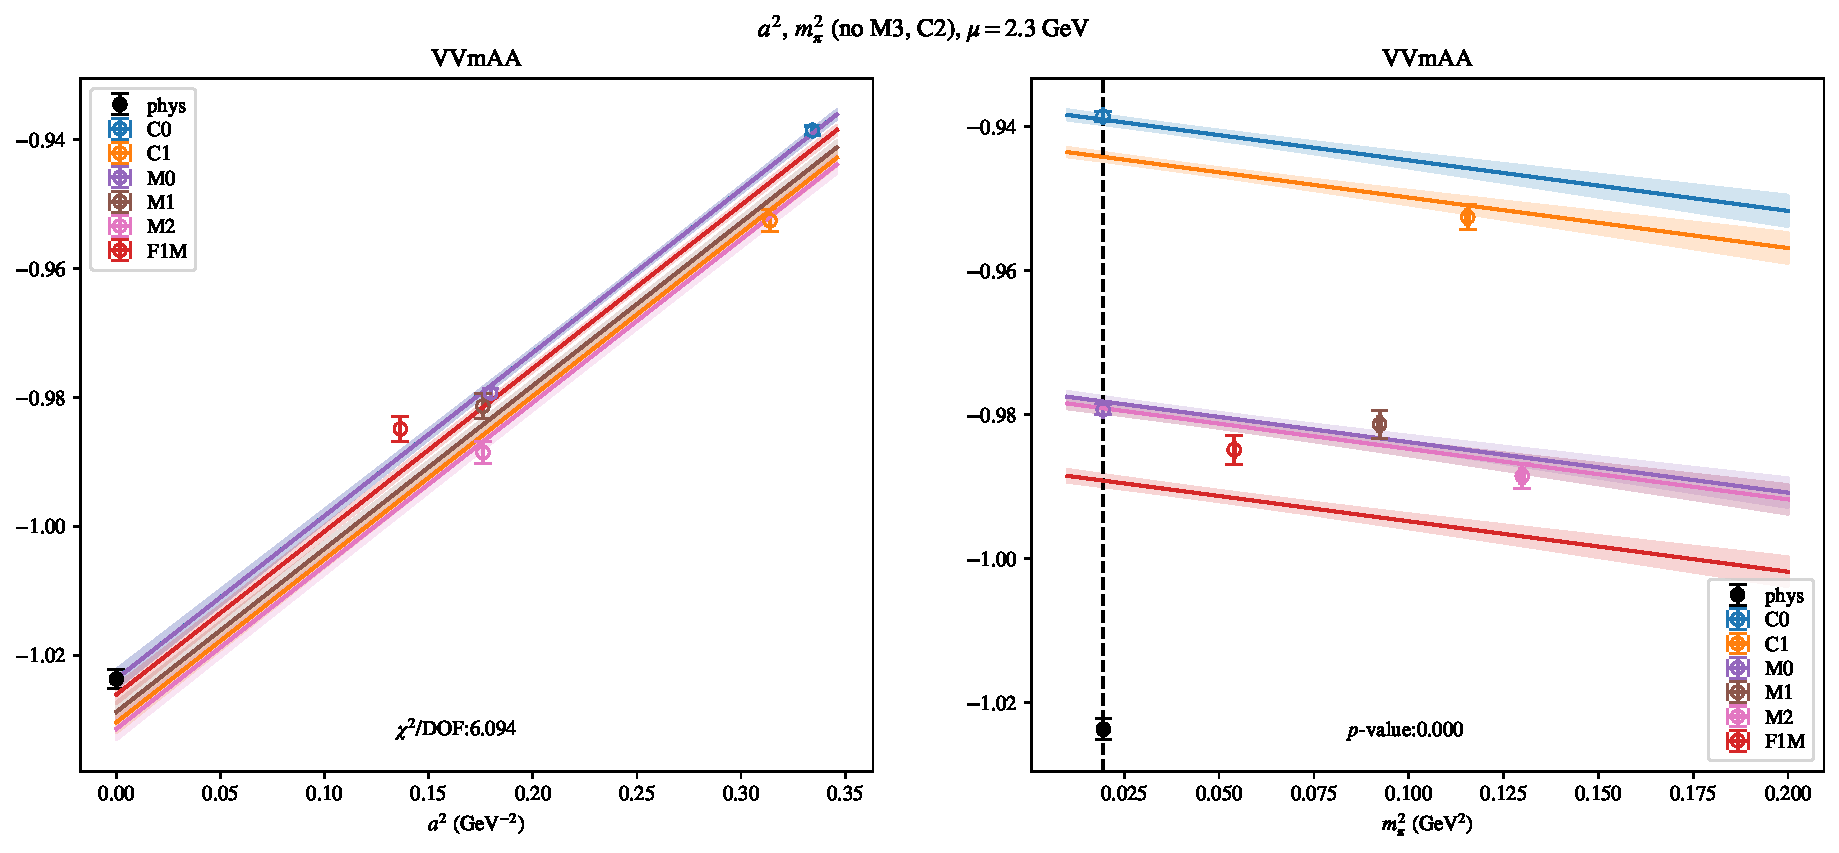
\includepdf[link, pages=-]{VVmAA/NPR/a2m2mcut_23.pdf}
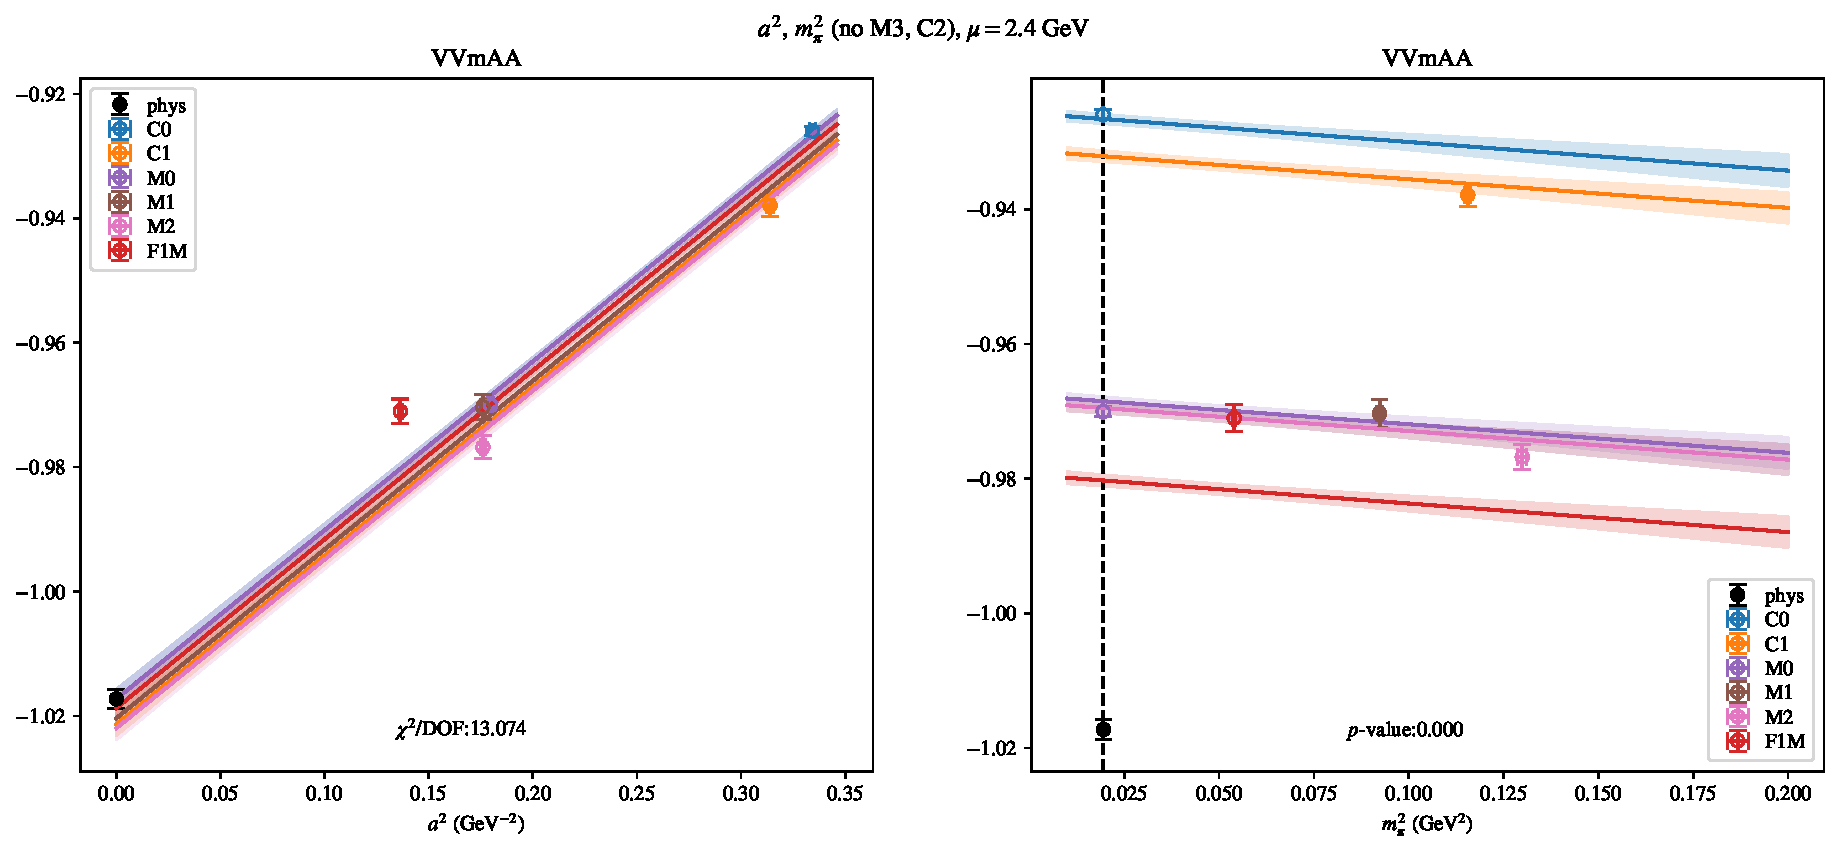
\includepdf[link, pages=-]{VVmAA/NPR/a2m2mcut_24.pdf}
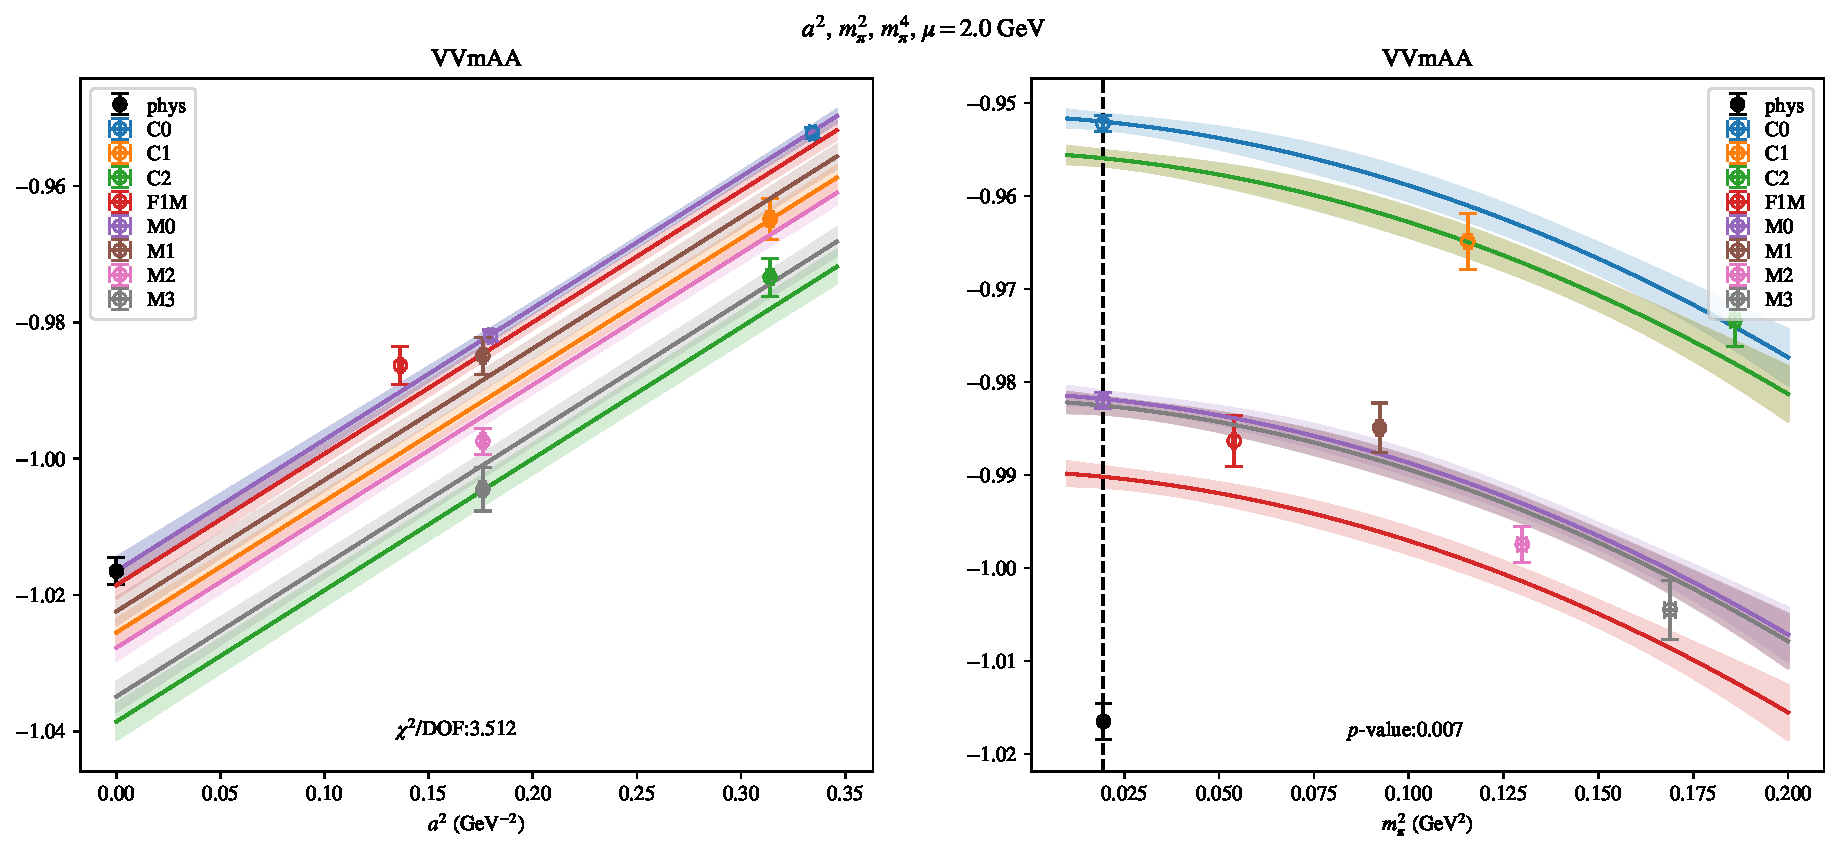
\includepdf[link, pages=-]{VVmAA/NPR/a2m2m4_20.pdf}
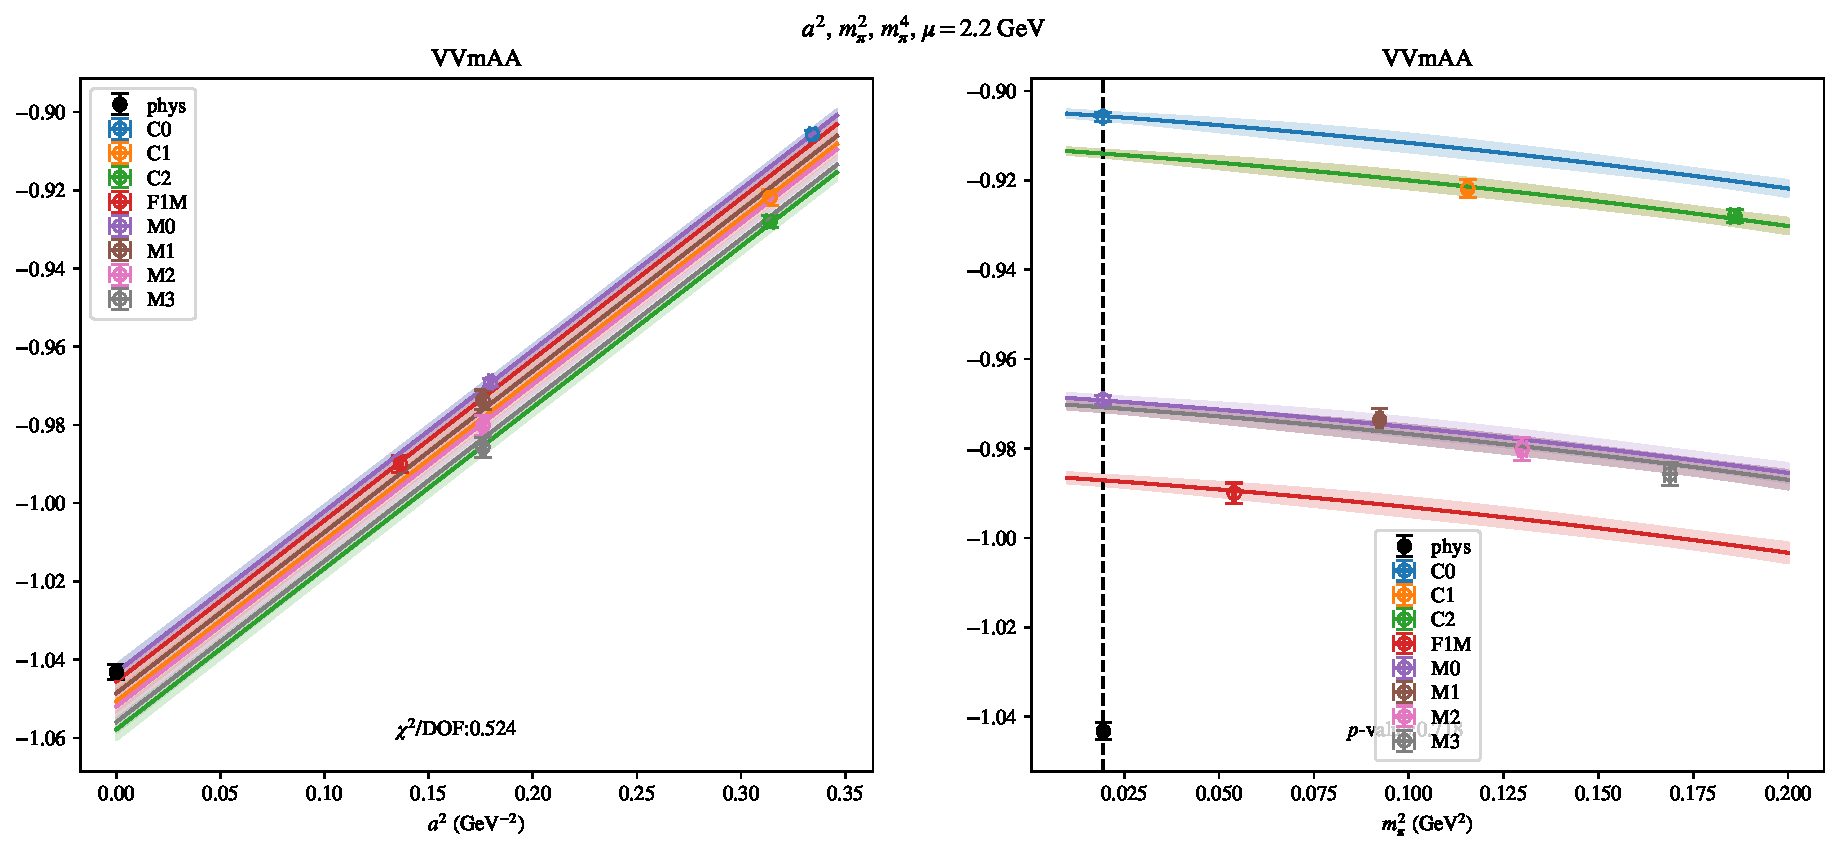
\includepdf[link, pages=-]{VVmAA/NPR/a2m2m4_22.pdf}
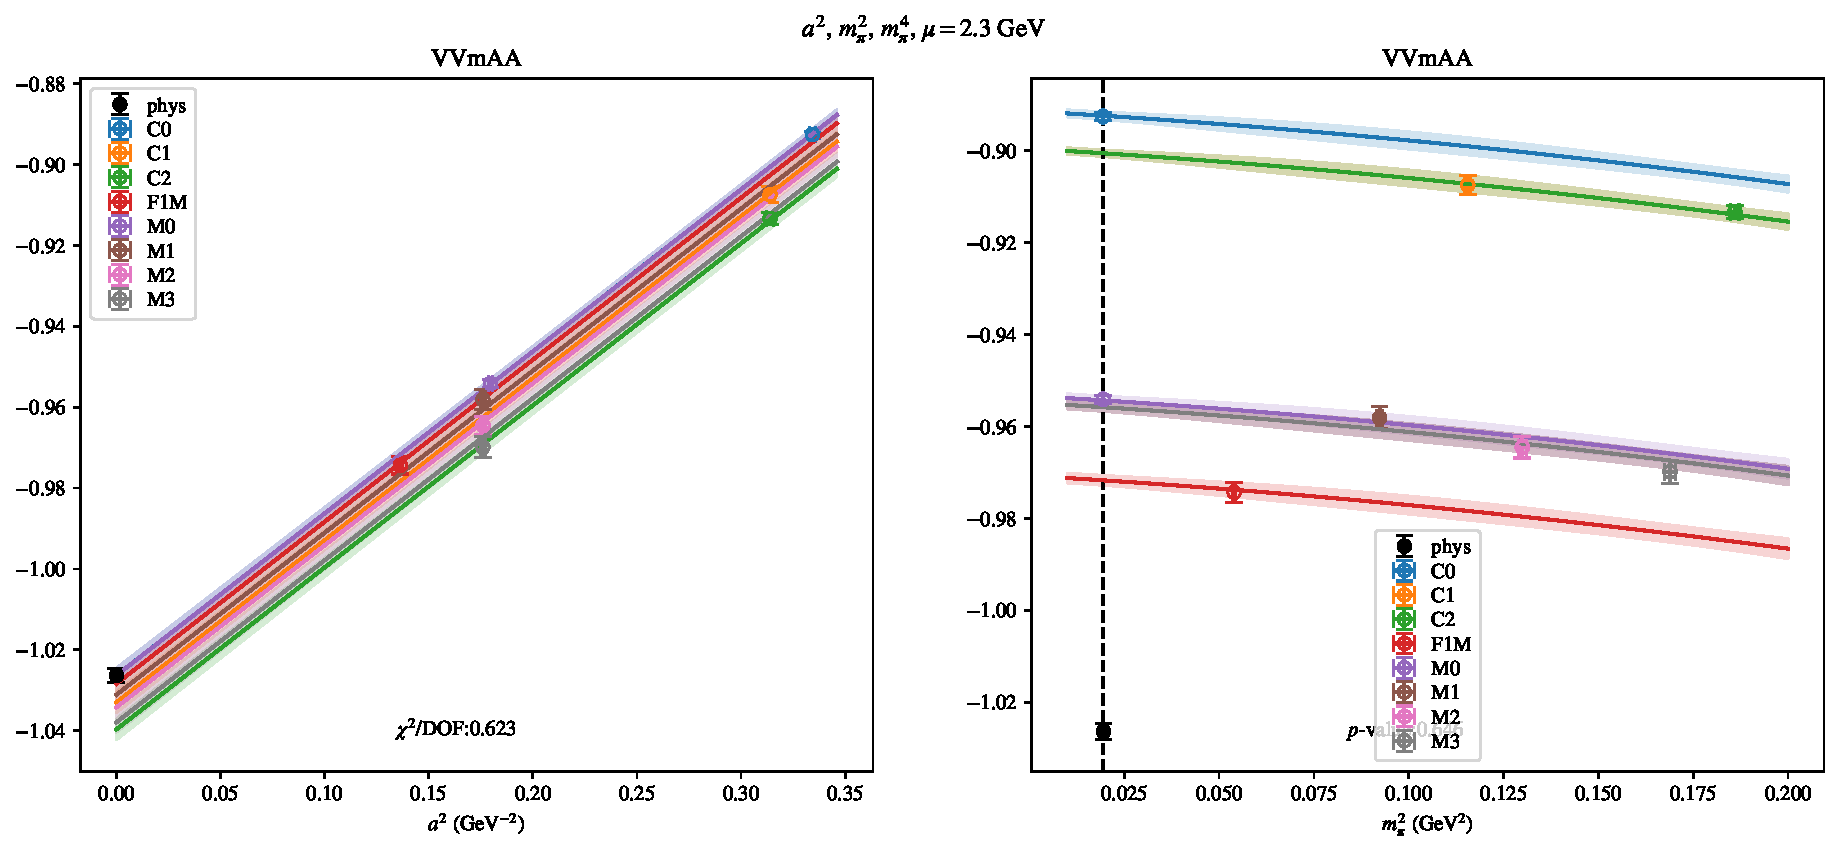
\includepdf[link, pages=-]{VVmAA/NPR/a2m2m4_23.pdf}
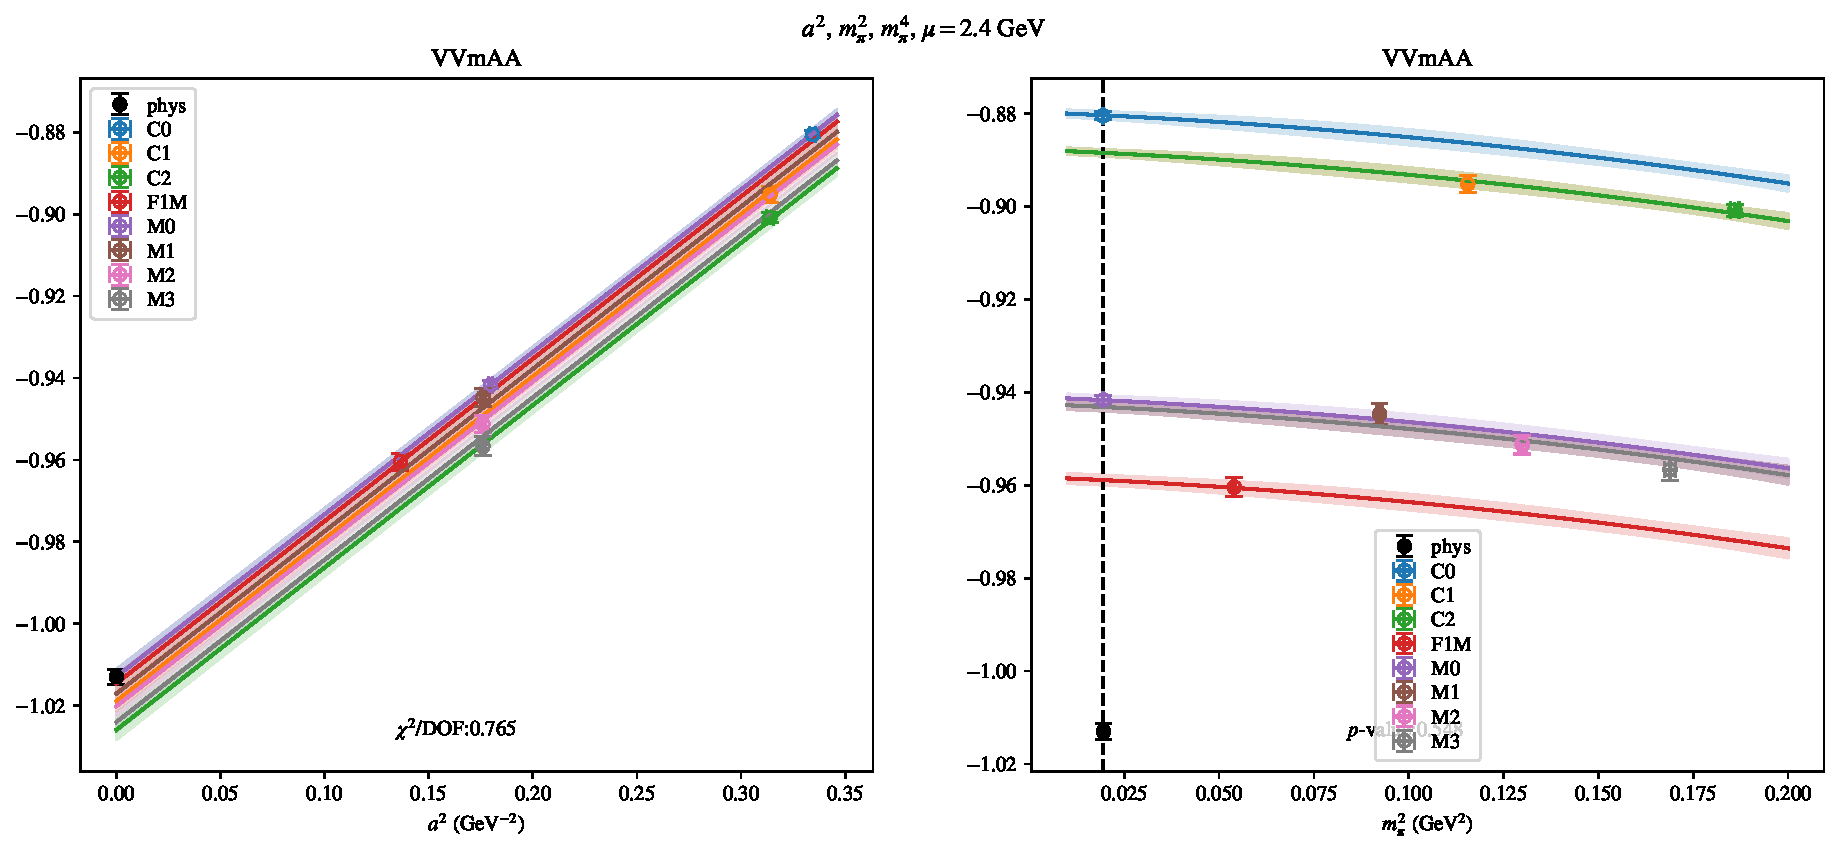
\includepdf[link, pages=-]{VVmAA/NPR/a2m2m4_24.pdf}
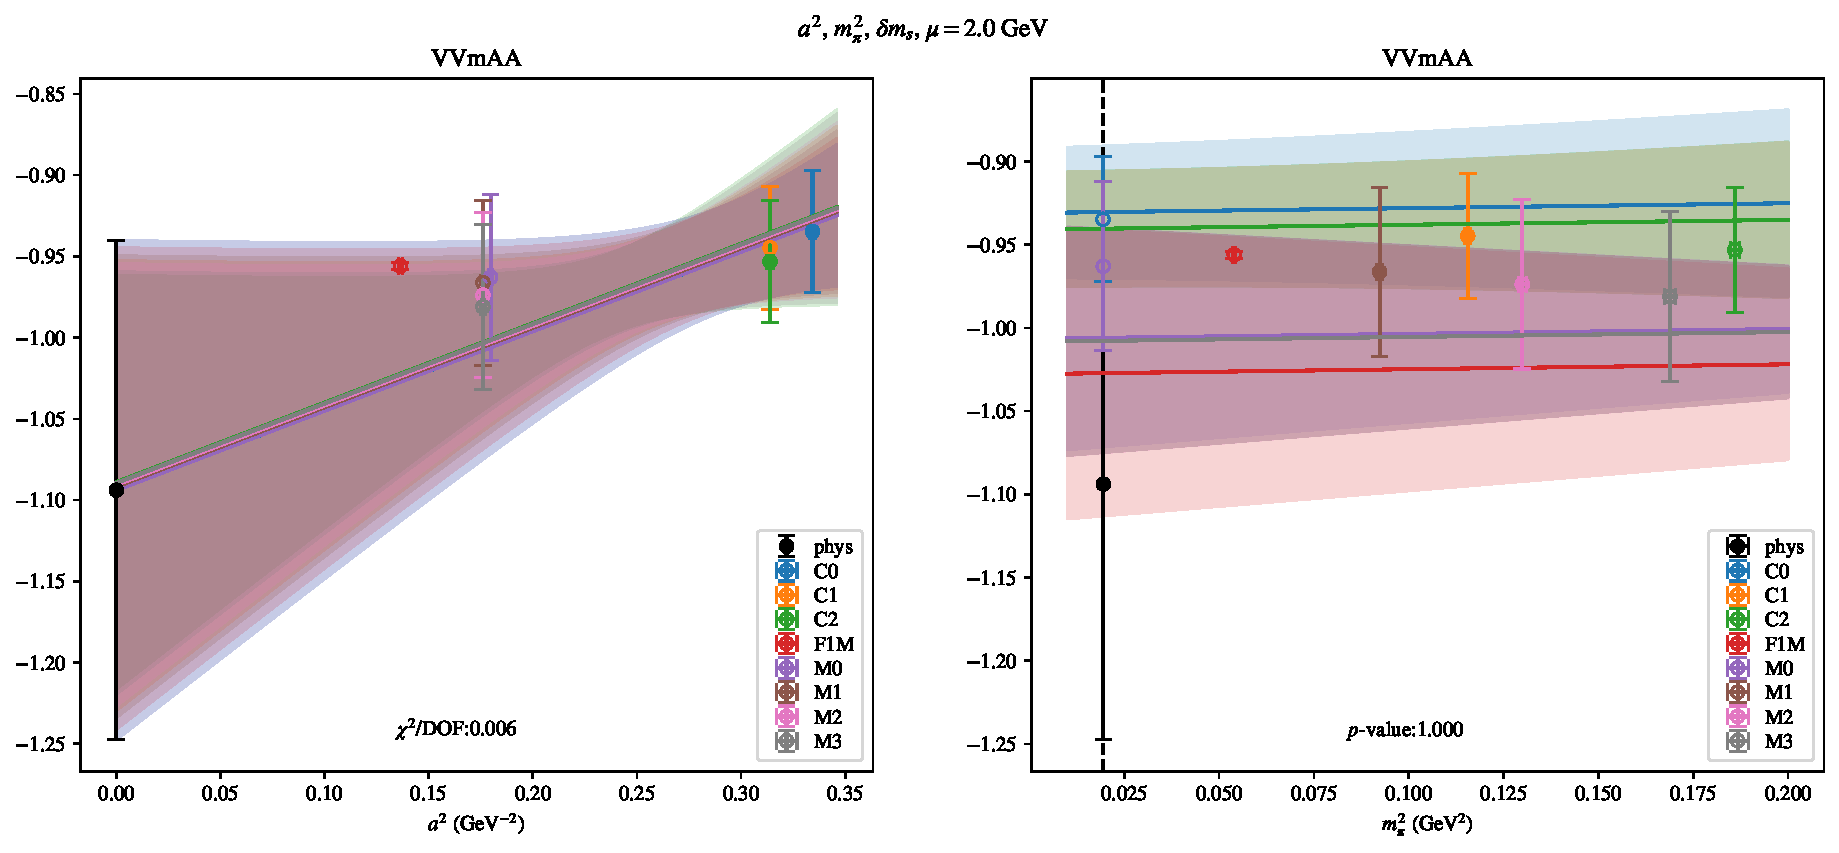
\includepdf[link, pages=-]{VVmAA/NPR/a2m2delm_20.pdf}
\includepdf[link, pages=-]{VVmAA/NPR/a2m2delm_22.pdf}
\includepdf[link, pages=-]{VVmAA/NPR/a2m2delm_23.pdf}
\includepdf[link, pages=-]{VVmAA/NPR/a2m2delm_24.pdf}
\clearpage
\section{$\mathcal{B}_3$}
\begin{table}[h!]
\begin{center}
\begin{tabular}{|c|c|c|c|c|c|c|}
\hline
$\mu$ (GeV) & $a^2$, $m_\pi^2$& $a^2$, $m_\pi^2$ (no C)& $a^2$, $m_\pi^2$, $a^4$& $a^2$, $m_\pi^2$ (no M3, C2)& $a^2$, $m_\pi^2$, $m_\pi^4$& $a^2$, $m_\pi^2$, $\delta m_s$\\
\hline
2.0& \hyperlink{SSmPP/NPR/a2m2_20.pdf.1}{\textbf{1.7999(28)}: 15.687 (0.0)} & \hyperlink{SSmPP/NPR/a2m2noC_20.pdf.1}{\textbf{1.693(13)}: 0.636 (0.529)} & \hyperlink{SSmPP/NPR/a2a4m2_20.pdf.1}{\textbf{1.606(22)}: 1.004 (0.404)} & \hyperlink{SSmPP/NPR/a2m2mcut_20.pdf.1}{\textbf{1.8039(40)}: 24.728 (0.0)} & \hyperlink{SSmPP/NPR/a2m2m4_20.pdf.1}{\textbf{1.8061(33)}: 15.171 (0.0)} & \hyperlink{SSmPP/NPR/a2m2delm_20.pdf.1}{\textbf{1.8091(30)}: 1.263 (0.282)}\\
2.2& \hyperlink{SSmPP/NPR/a2m2_22.pdf.1}{\textbf{1.8057(27)}: 14.641 (0.0)} & \hyperlink{SSmPP/NPR/a2m2noC_22.pdf.1}{\textbf{1.703(12)}: 1.333 (0.264)} & \hyperlink{SSmPP/NPR/a2a4m2_22.pdf.1}{\textbf{1.626(21)}: 1.471 (0.208)} & \hyperlink{SSmPP/NPR/a2m2mcut_22.pdf.1}{\textbf{1.8094(40)}: 21.997 (0.0)} & \hyperlink{SSmPP/NPR/a2m2m4_22.pdf.1}{\textbf{1.8120(33)}: 13.264 (0.0)} & \hyperlink{SSmPP/NPR/a2m2delm_22.pdf.1}{\textbf{1.8141(29)}: 2.142 (0.073)}\\
2.3& \hyperlink{SSmPP/NPR/a2m2_23.pdf.1}{\textbf{1.8079(26)}: 14.085 (0.0)} & \hyperlink{SSmPP/NPR/a2m2noC_23.pdf.1}{\textbf{1.708(12)}: 1.49 (0.225)} & \hyperlink{SSmPP/NPR/a2a4m2_23.pdf.1}{\textbf{1.631(21)}: 1.37 (0.241)} & \hyperlink{SSmPP/NPR/a2m2mcut_23.pdf.1}{\textbf{1.8116(39)}: 21.382 (0.0)} & \hyperlink{SSmPP/NPR/a2m2m4_23.pdf.1}{\textbf{1.8142(33)}: 13.09 (0.0)} & \hyperlink{SSmPP/NPR/a2m2delm_23.pdf.1}{\textbf{1.8160(28)}: 2.203 (0.066)}\\
2.4& \hyperlink{SSmPP/NPR/a2m2_24.pdf.1}{\textbf{1.8092(26)}: 13.072 (0.0)} & \hyperlink{SSmPP/NPR/a2m2noC_24.pdf.1}{\textbf{1.712(12)}: 1.5 (0.223)} & \hyperlink{SSmPP/NPR/a2a4m2_24.pdf.1}{\textbf{1.638(21)}: 1.362 (0.244)} & \hyperlink{SSmPP/NPR/a2m2mcut_24.pdf.1}{\textbf{1.8128(38)}: 19.976 (0.0)} & \hyperlink{SSmPP/NPR/a2m2m4_24.pdf.1}{\textbf{1.8152(32)}: 12.362 (0.0)} & \hyperlink{SSmPP/NPR/a2m2delm_24.pdf.1}{\textbf{1.8168(27)}: 2.127 (0.075)}\\
\hline
\end{tabular}
\caption{Physical point value from chiral and continuum extrapolation at renormalisation scale $\mu$. Entries are \textbf{value(error)}: $\chi^2/\text{DOF}$ ($p$-value).}
\end{center}
\end{table}
\begin{table}[h!]
\begin{center}
\begin{tabular}{|c c|c|c|c|c|c|c|}
\hline
$\mu$ (GeV) &  & $a^2$, $m_\pi^2$& $a^2$, $m_\pi^2$ (no C)& $a^2$, $m_\pi^2$, $a^4$& $a^2$, $m_\pi^2$ (no M3, C2)& $a^2$, $m_\pi^2$, $m_\pi^4$& $a^2$, $m_\pi^2$, $\delta m_s$\\
\hline
\multirow{3}{0.5in}{2.0} & $\alpha$ & 0.0698(62)& 0.443(47)& 1.15(13)& 0.0617(97)& 0.0582(75)& 0.0507(66)\\
 & $\beta$ & -0.0011(13)& -0.0016(54)& -0.0015(15)& -0.0016(30)& -0.004(10)& -0.0014(13)\\
 & $\gamma$ &  &  & -2.1(27)&  & 0.000335(94)& 0.0156(17)\\
\hline
\multirow{3}{0.5in}{2.2} & $\alpha$ & 0.0748(62)& 0.430(45)& 1.07(13)& 0.0676(95)& 0.0632(76)& 0.0573(66)\\
 & $\beta$ & -0.0007(12)& -0.0011(35)& -0.0011(14)& -0.0014(27)& -0.0044(97)& -0.0010(12)\\
 & $\gamma$ &  &  & -1.9(26)&  & 0.000326(87)& 0.0144(17)\\
\hline
\multirow{3}{0.5in}{2.3} & $\alpha$ & 0.0760(61)& 0.424(45)& 1.05(13)& 0.0689(95)& 0.0646(76)& 0.0594(65)\\
 & $\beta$ & -0.0006(12)& -0.0010(32)& -0.0010(13)& -0.0013(26)& -0.0041(93)& -0.0009(12)\\
 & $\gamma$ &  &  & -1.9(26)&  & 0.000305(84)& 0.0140(17)\\
\hline
\multirow{3}{0.5in}{2.4} & $\alpha$ & 0.0781(59)& 0.413(44)& 1.02(13)& 0.0710(93)& 0.0670(74)& 0.0625(63)\\
 & $\beta$ & -0.0006(12)& -0.0010(31)& -0.0010(13)& -0.0011(24)& -0.0037(87)& -0.0009(12)\\
 & $\gamma$ &  &  & -1.8(26)&  & 0.000281(80)& 0.0135(17)\\
\hline
\end{tabular}
\caption{Fit values of coefficients in $Q = Q_{phys} + \mathbf{\alpha} a^2 + \mathbf{\beta}\left(\frac{m_\pi^2}{f_\pi^2}-\frac{m_{\pi,PDG}^2}{f_\pi^2}\right) + \gamma(\ldots)$}
\end{center}
\end{table}
\includepdf[link, pages=-]{SSmPP/NPR/a2m2_20.pdf}
\includepdf[link, pages=-]{SSmPP/NPR/a2m2_22.pdf}
\includepdf[link, pages=-]{SSmPP/NPR/a2m2_23.pdf}
\includepdf[link, pages=-]{SSmPP/NPR/a2m2_24.pdf}
\includepdf[link, pages=-]{SSmPP/NPR/a2m2noC_20.pdf}
\includepdf[link, pages=-]{SSmPP/NPR/a2m2noC_22.pdf}
\includepdf[link, pages=-]{SSmPP/NPR/a2m2noC_23.pdf}
\includepdf[link, pages=-]{SSmPP/NPR/a2m2noC_24.pdf}
\includepdf[link, pages=-]{SSmPP/NPR/a2a4m2_20.pdf}
\includepdf[link, pages=-]{SSmPP/NPR/a2a4m2_22.pdf}
\includepdf[link, pages=-]{SSmPP/NPR/a2a4m2_23.pdf}
\includepdf[link, pages=-]{SSmPP/NPR/a2a4m2_24.pdf}
\includepdf[link, pages=-]{SSmPP/NPR/a2m2mcut_20.pdf}
\includepdf[link, pages=-]{SSmPP/NPR/a2m2mcut_22.pdf}
\includepdf[link, pages=-]{SSmPP/NPR/a2m2mcut_23.pdf}
\includepdf[link, pages=-]{SSmPP/NPR/a2m2mcut_24.pdf}
\includepdf[link, pages=-]{SSmPP/NPR/a2m2m4_20.pdf}
\includepdf[link, pages=-]{SSmPP/NPR/a2m2m4_22.pdf}
\includepdf[link, pages=-]{SSmPP/NPR/a2m2m4_23.pdf}
\includepdf[link, pages=-]{SSmPP/NPR/a2m2m4_24.pdf}
\includepdf[link, pages=-]{SSmPP/NPR/a2m2delm_20.pdf}
\includepdf[link, pages=-]{SSmPP/NPR/a2m2delm_22.pdf}
\includepdf[link, pages=-]{SSmPP/NPR/a2m2delm_23.pdf}
\includepdf[link, pages=-]{SSmPP/NPR/a2m2delm_24.pdf}
\clearpage
\section{$\mathcal{B}_4$}
\begin{table}[h!]
\begin{center}
\begin{tabular}{|c|c|c|c|c|c|c|}
\hline
$\mu$ (GeV) & $a^2$, $m_\pi^2$& $a^2$, $m_\pi^2$ (no C)& $a^2$, $m_\pi^2$, $a^4$& $a^2$, $m_\pi^2$ (no M3, C2)& $a^2$, $m_\pi^2$, $m_\pi^4$& $a^2$, $m_\pi^2$, $\delta m_s$\\
\hline
2.0& \hyperlink{SSpPP/NPR/a2m2_20.pdf.1}{\textbf{-0.924(19)}: 2.927 (0.012)} & \hyperlink{SSpPP/NPR/a2m2noC_20.pdf.1}{\textbf{-0.937(97)}: 2.436 (0.088)} & \hyperlink{SSpPP/NPR/a2a4m2_20.pdf.1}{\textbf{-0.92(16)}: 3.659 (0.006)} & \hyperlink{SSpPP/NPR/a2m2mcut_20.pdf.1}{\textbf{-0.924(19)}: 3.205 (0.022)} & \hyperlink{SSpPP/NPR/a2m2m4_20.pdf.1}{\textbf{-0.923(19)}: 2.638 (0.032)} & \hyperlink{SSpPP/NPR/a2m2delm_20.pdf.1}{\textbf{-0.923(22)}: 3.591 (0.006)}\\
2.2& \hyperlink{SSpPP/NPR/a2m2_22.pdf.1}{\textbf{-0.905(16)}: 4.022 (0.001)} & \hyperlink{SSpPP/NPR/a2m2noC_22.pdf.1}{\textbf{-0.918(88)}: 2.014 (0.133)} & \hyperlink{SSpPP/NPR/a2a4m2_22.pdf.1}{\textbf{-0.91(16)}: 5.028 (0.0)} & \hyperlink{SSpPP/NPR/a2m2mcut_22.pdf.1}{\textbf{-0.904(19)}: 4.273 (0.005)} & \hyperlink{SSpPP/NPR/a2m2m4_22.pdf.1}{\textbf{-0.904(18)}: 4.239 (0.002)} & \hyperlink{SSpPP/NPR/a2m2delm_22.pdf.1}{\textbf{-0.904(17)}: 4.78 (0.001)}\\
2.3& \hyperlink{SSpPP/NPR/a2m2_23.pdf.1}{\textbf{-0.896(16)}: 4.51 (0.0)} & \hyperlink{SSpPP/NPR/a2m2noC_23.pdf.1}{\textbf{-0.911(86)}: 2.336 (0.097)} & \hyperlink{SSpPP/NPR/a2a4m2_23.pdf.1}{\textbf{-0.90(16)}: 5.631 (0.0)} & \hyperlink{SSpPP/NPR/a2m2mcut_23.pdf.1}{\textbf{-0.895(20)}: 4.959 (0.002)} & \hyperlink{SSpPP/NPR/a2m2m4_23.pdf.1}{\textbf{-0.895(18)}: 4.656 (0.001)} & \hyperlink{SSpPP/NPR/a2m2delm_23.pdf.1}{\textbf{-0.895(17)}: 5.29 (0.0)}\\
2.4& \hyperlink{SSpPP/NPR/a2m2_24.pdf.1}{\textbf{-0.888(15)}: 4.902 (0.0)} & \hyperlink{SSpPP/NPR/a2m2noC_24.pdf.1}{\textbf{-0.904(85)}: 2.488 (0.083)} & \hyperlink{SSpPP/NPR/a2a4m2_24.pdf.1}{\textbf{-0.90(16)}: 6.124 (0.0)} & \hyperlink{SSpPP/NPR/a2m2mcut_24.pdf.1}{\textbf{-0.888(20)}: 5.532 (0.001)} & \hyperlink{SSpPP/NPR/a2m2m4_24.pdf.1}{\textbf{-0.887(17)}: 5.171 (0.0)} & \hyperlink{SSpPP/NPR/a2m2delm_24.pdf.1}{\textbf{-0.887(16)}: 5.76 (0.0)}\\
\hline
\end{tabular}
\caption{Physical point value from chiral and continuum extrapolation at renormalisation scale $\mu$. Entries are \textbf{value(error)}: $\chi^2/\text{DOF}$ ($p$-value).}
\end{center}
\end{table}
\begin{table}[h!]
\begin{center}
\begin{tabular}{|c c|c|c|c|c|c|c|}
\hline
$\mu$ (GeV) &  & $a^2$, $m_\pi^2$& $a^2$, $m_\pi^2$ (no C)& $a^2$, $m_\pi^2$, $a^4$& $a^2$, $m_\pi^2$ (no M3, C2)& $a^2$, $m_\pi^2$, $m_\pi^4$& $a^2$, $m_\pi^2$, $\delta m_s$\\
\hline
\multirow{3}{0.5in}{2.0} & $\alpha$ & 0.3851(95)& 0.303(63)& 0.34(16)& 0.3842(94)& 0.3890(93)& 0.387(10)\\
 & $\beta$ & 0.00645(21)& 0.00590(39)& 0.00643(23)& 0.00671(39)& 0.0075(10)& 0.00651(20)\\
 & $\gamma$ &  &  & 0.083&  & -0.00010(90)& -0.002(28)\\
\hline
\multirow{3}{0.5in}{2.2} & $\alpha$ & 0.4284(78)& 0.343(58)& 0.33(17)& 0.4297(97)& 0.4312(86)& 0.4313(83)\\
 & $\beta$ & 0.00691(17)& 0.00656(29)& 0.00687(20)& 0.00705(37)& 0.0077(10)& 0.00699(17)\\
 & $\gamma$ &  &  & 0.17(34)&  & -7.06546(85)& -0.003(26)\\
\hline
\multirow{3}{0.5in}{2.3} & $\alpha$ & 0.4507(77)& 0.351(57)& 0.32(17)& 0.452(10)& 0.4539(85)& 0.4540(83)\\
 & $\beta$ & 0.00701(16)& 0.00666(29)& 0.00696(20)& 0.00715(38)& 0.0078(10)& 0.00710(16)\\
 & $\gamma$ &  &  & 0.23(34)&  & -7.65679(90)& -0.003(26)\\
\hline
\multirow{3}{0.5in}{2.4} & $\alpha$ & 0.4703(78)& 0.365(57)& 0.34(18)& 0.472(10)& 0.4738(84)& 0.4737(84)\\
 & $\beta$ & 0.00711(16)& 0.00673(28)& 0.00705(20)& 0.00726(35)& 0.0080(10)& 0.00721(16)\\
 & $\gamma$ &  &  & 0.24(34)&  & -7.91721(86)& -0.003(26)\\
\hline
\end{tabular}
\caption{Fit values of coefficients in $Q = Q_{phys} + \mathbf{\alpha} a^2 + \mathbf{\beta}\left(\frac{m_\pi^2}{f_\pi^2}-\frac{m_{\pi,PDG}^2}{f_\pi^2}\right) + \gamma(\ldots)$}
\end{center}
\end{table}
\includepdf[link, pages=-]{SSpPP/NPR/a2m2_20.pdf}
\includepdf[link, pages=-]{SSpPP/NPR/a2m2_22.pdf}
\includepdf[link, pages=-]{SSpPP/NPR/a2m2_23.pdf}
\includepdf[link, pages=-]{SSpPP/NPR/a2m2_24.pdf}
\includepdf[link, pages=-]{SSpPP/NPR/a2m2noC_20.pdf}
\includepdf[link, pages=-]{SSpPP/NPR/a2m2noC_22.pdf}
\includepdf[link, pages=-]{SSpPP/NPR/a2m2noC_23.pdf}
\includepdf[link, pages=-]{SSpPP/NPR/a2m2noC_24.pdf}
\includepdf[link, pages=-]{SSpPP/NPR/a2a4m2_20.pdf}
\includepdf[link, pages=-]{SSpPP/NPR/a2a4m2_22.pdf}
\includepdf[link, pages=-]{SSpPP/NPR/a2a4m2_23.pdf}
\includepdf[link, pages=-]{SSpPP/NPR/a2a4m2_24.pdf}
\includepdf[link, pages=-]{SSpPP/NPR/a2m2mcut_20.pdf}
\includepdf[link, pages=-]{SSpPP/NPR/a2m2mcut_22.pdf}
\includepdf[link, pages=-]{SSpPP/NPR/a2m2mcut_23.pdf}
\includepdf[link, pages=-]{SSpPP/NPR/a2m2mcut_24.pdf}
\includepdf[link, pages=-]{SSpPP/NPR/a2m2m4_20.pdf}
\includepdf[link, pages=-]{SSpPP/NPR/a2m2m4_22.pdf}
\includepdf[link, pages=-]{SSpPP/NPR/a2m2m4_23.pdf}
\includepdf[link, pages=-]{SSpPP/NPR/a2m2m4_24.pdf}
\includepdf[link, pages=-]{SSpPP/NPR/a2m2delm_20.pdf}
\includepdf[link, pages=-]{SSpPP/NPR/a2m2delm_22.pdf}
\includepdf[link, pages=-]{SSpPP/NPR/a2m2delm_23.pdf}
\includepdf[link, pages=-]{SSpPP/NPR/a2m2delm_24.pdf}
\clearpage
\section{$\mathcal{B}_5$}
\begin{table}[h!]
\begin{center}
\begin{tabular}{|c|c|c|c|c|c|c|}
\hline
$\mu$ (GeV) & $a^2$, $m_\pi^2$& $a^2$, $m_\pi^2$ (no C)& $a^2$, $m_\pi^2$, $a^4$& $a^2$, $m_\pi^2$ (no M3, C2)& $a^2$, $m_\pi^2$, $m_\pi^4$& $a^2$, $m_\pi^2$, $\delta m_s$\\
\hline
2.0& \hyperlink{TT/NPR/a2m2_20.pdf.1}{\textbf{-0.3622(78)}: 0.611 (0.691)} & \hyperlink{TT/NPR/a2m2noC_20.pdf.1}{\textbf{-0.365(45)}: 0.131 (0.878)} & \hyperlink{TT/NPR/a2a4m2_20.pdf.1}{\textbf{-0.360(72)}: 0.748 (0.559)} & \hyperlink{TT/NPR/a2m2mcut_20.pdf.1}{\textbf{-0.3625(75)}: 0.693 (0.556)} & \hyperlink{TT/NPR/a2m2m4_20.pdf.1}{\textbf{-0.3624(75)}: 0.65 (0.627)} & \hyperlink{TT/NPR/a2m2delm_20.pdf.1}{\textbf{-0.3621(85)}: 0.755 (0.554)}\\
2.2& \hyperlink{TT/NPR/a2m2_22.pdf.1}{\textbf{-0.3598(68)}: 0.963 (0.439)} & \hyperlink{TT/NPR/a2m2noC_22.pdf.1}{\textbf{-0.362(40)}: 0.265 (0.767)} & \hyperlink{TT/NPR/a2a4m2_22.pdf.1}{\textbf{-0.360(72)}: 1.193 (0.312)} & \hyperlink{TT/NPR/a2m2mcut_22.pdf.1}{\textbf{-0.3599(73)}: 1.37 (0.25)} & \hyperlink{TT/NPR/a2m2m4_22.pdf.1}{\textbf{-0.3600(76)}: 1.198 (0.309)} & \hyperlink{TT/NPR/a2m2delm_22.pdf.1}{\textbf{-0.3597(71)}: 1.137 (0.337)}\\
2.3& \hyperlink{TT/NPR/a2m2_23.pdf.1}{\textbf{-0.3587(66)}: 1.02 (0.404)} & \hyperlink{TT/NPR/a2m2noC_23.pdf.1}{\textbf{-0.361(39)}: 0.353 (0.702)} & \hyperlink{TT/NPR/a2a4m2_23.pdf.1}{\textbf{-0.359(71)}: 1.267 (0.28)} & \hyperlink{TT/NPR/a2m2mcut_23.pdf.1}{\textbf{-0.3587(72)}: 1.519 (0.207)} & \hyperlink{TT/NPR/a2m2m4_23.pdf.1}{\textbf{-0.3589(75)}: 1.171 (0.321)} & \hyperlink{TT/NPR/a2m2delm_23.pdf.1}{\textbf{-0.3586(69)}: 1.229 (0.296)}\\
2.4& \hyperlink{TT/NPR/a2m2_24.pdf.1}{\textbf{-0.3578(65)}: 0.951 (0.447)} & \hyperlink{TT/NPR/a2m2noC_24.pdf.1}{\textbf{-0.360(38)}: 0.478 (0.62)} & \hyperlink{TT/NPR/a2a4m2_24.pdf.1}{\textbf{-0.359(71)}: 1.186 (0.314)} & \hyperlink{TT/NPR/a2m2mcut_24.pdf.1}{\textbf{-0.3577(72)}: 1.402 (0.24)} & \hyperlink{TT/NPR/a2m2m4_24.pdf.1}{\textbf{-0.3579(74)}: 0.979 (0.418)} & \hyperlink{TT/NPR/a2m2delm_24.pdf.1}{\textbf{-0.3577(69)}: 1.152 (0.33)}\\
\hline
\end{tabular}
\caption{Physical point value from chiral and continuum extrapolation at renormalisation scale $\mu$. Entries are \textbf{value(error)}: $\chi^2/\text{DOF}$ ($p$-value).}
\end{center}
\end{table}
\begin{table}[h!]
\begin{center}
\begin{tabular}{|c c|c|c|c|c|c|c|}
\hline
$\mu$ (GeV) &  & $a^2$, $m_\pi^2$& $a^2$, $m_\pi^2$ (no C)& $a^2$, $m_\pi^2$, $a^4$& $a^2$, $m_\pi^2$ (no M3, C2)& $a^2$, $m_\pi^2$, $m_\pi^4$& $a^2$, $m_\pi^2$, $\delta m_s$\\
\hline
\multirow{3}{0.5in}{2.0} & $\alpha$ & -0.035(86)& -0.07(71)& 0.004& -0.038(82)& -0.036(81)& -0.034(93)\\
 & $\beta$ & 0.00616(15)& 0.00567(38)& 0.00617(17)& 0.00601(40)& 0.0054(14)& 0.00620(17)\\
 & $\gamma$ &  &  & -0.078&  & 0.0& -0.001(35)\\
\hline
\multirow{3}{0.5in}{2.2} & $\alpha$ & -0.081(76)& -0.12(62)& -0.097& -0.081(80)& -0.082(84)& -0.079(78)\\
 & $\beta$ & 0.00629(14)& 0.00601(25)& 0.00628(17)& 0.00610(31)& 0.0056(10)& 0.00634(15)\\
 & $\gamma$ &  &  & 0.031&  & 5.647284(90)& -0.002(31)\\
\hline
\multirow{3}{0.5in}{2.3} & $\alpha$ & -0.104(73)& -0.14(61)& -0.1(18)& -0.103(79)& -0.106(81)& -0.103(76)\\
 & $\beta$ & 0.00629(14)& 0.00607(24)& 0.00628(17)& 0.00614(34)& 0.0058(11)& 0.00634(15)\\
 & $\gamma$ &  &  & 0.045&  & 4.019354(99)& -0.002(31)\\
\hline
\multirow{3}{0.5in}{2.4} & $\alpha$ & -0.129(72)& -0.16(60)& -0.1(17)& -0.127(78)& -0.130(81)& -0.128(74)\\
 & $\beta$ & 0.00626(14)& 0.00612(24)& 0.00624(16)& 0.00615(34)& 0.0059(11)& 0.00631(15)\\
 & $\gamma$ &  &  & 0.072&  & 0.0& -0.002(31)\\
\hline
\end{tabular}
\caption{Fit values of coefficients in $Q = Q_{phys} + \mathbf{\alpha} a^2 + \mathbf{\beta}\left(\frac{m_\pi^2}{f_\pi^2}-\frac{m_{\pi,PDG}^2}{f_\pi^2}\right) + \gamma(\ldots)$}
\end{center}
\end{table}
\includepdf[link, pages=-]{TT/NPR/a2m2_20.pdf}
\includepdf[link, pages=-]{TT/NPR/a2m2_22.pdf}
\includepdf[link, pages=-]{TT/NPR/a2m2_23.pdf}
\includepdf[link, pages=-]{TT/NPR/a2m2_24.pdf}
\includepdf[link, pages=-]{TT/NPR/a2m2noC_20.pdf}
\includepdf[link, pages=-]{TT/NPR/a2m2noC_22.pdf}
\includepdf[link, pages=-]{TT/NPR/a2m2noC_23.pdf}
\includepdf[link, pages=-]{TT/NPR/a2m2noC_24.pdf}
\includepdf[link, pages=-]{TT/NPR/a2a4m2_20.pdf}
\includepdf[link, pages=-]{TT/NPR/a2a4m2_22.pdf}
\includepdf[link, pages=-]{TT/NPR/a2a4m2_23.pdf}
\includepdf[link, pages=-]{TT/NPR/a2a4m2_24.pdf}
\includepdf[link, pages=-]{TT/NPR/a2m2mcut_20.pdf}
\includepdf[link, pages=-]{TT/NPR/a2m2mcut_22.pdf}
\includepdf[link, pages=-]{TT/NPR/a2m2mcut_23.pdf}
\includepdf[link, pages=-]{TT/NPR/a2m2mcut_24.pdf}
\includepdf[link, pages=-]{TT/NPR/a2m2m4_20.pdf}
\includepdf[link, pages=-]{TT/NPR/a2m2m4_22.pdf}
\includepdf[link, pages=-]{TT/NPR/a2m2m4_23.pdf}
\includepdf[link, pages=-]{TT/NPR/a2m2m4_24.pdf}
\includepdf[link, pages=-]{TT/NPR/a2m2delm_20.pdf}
\includepdf[link, pages=-]{TT/NPR/a2m2delm_22.pdf}
\includepdf[link, pages=-]{TT/NPR/a2m2delm_23.pdf}
\includepdf[link, pages=-]{TT/NPR/a2m2delm_24.pdf}
\clearpage
\end{document}